%&../preamble

\def\npart {IB}
\def\nterm {Michaelmas}
\def\nyear {2022}
\def\nlecturer {Dr E P Shellard}
\def\ncourse {Methods}

\def\encodingdefault{TU}\normalfont
\ifnum 0\ifxetex 1\fi\ifluatex 1\fi=0 % if pdftex
  \usepackage[T1]{fontenc}
  \usepackage[utf8]{inputenc}
  \usepackage{textcomp} % provide euro and other symbols
\else % if luatex or xetex
  % \usepackage{unicode-math}
  % \defaultfontfeatures{Scale=MatchLowercase}
  % \defaultfontfeatures[\rmfamily]{Ligatures=TeX,Scale=1}
  % \DeclareMathAlphabet{\mathcal}{OMS}{cmsy}{m}{n}
  % \let\mathbb\relax % remove the definition by unicode-math
  % \DeclareMathAlphabet{\mathbb}{U}{msb}{m}{n}
\fi

\usetikzlibrary{external}
\tikzset{external/system call={xelatex -fmt=../preamble.fmt \tikzexternalcheckshellescape -halt-on-error -interaction=batchmode -jobname "\image" "\texsource"}} % path is relative to file that includes preamble
\tikzexternalize

\providetoggle{DontSetTitleAuthorDate}

\nottoggle{DontSetTitleAuthorDate}{
  \hypersetup{
    pdftitle={Part \npart\ - \ncourse},
    pdfsubject={Cambridge Maths Notes: Part \npart\ - \ncourse},
    pdfkeywords={Cambridge Mathematics Maths Math \npart\ \nterm\ \nyear\ \ncourse}
  }

  \author{Based on lectures by \nlecturer}
  \date{\nterm\ \nyear}
  \title{Part \npart\ --- \ncourse}
}{}

\tikzsetexternalprefix{figtemp/}
% \newcommand{\norm}[1]{\left \lVert #1 \right \rVert}
\newcommand{\inv}{^{-1}}

\author{Based on lectures by \nlecturer \ and notes by thirdsgames.co.uk}
\numberwithin{equation}{section}

% \setcounter{section}{-1}

% \includeonly{05-Laplace.tex}

\begin{document}
    \maketitle
    \tableofcontents

    % \part{Self-Adjoint ODEs}
    \part{Self-Adjoint ODEs}

\section{Fourier Series}

\subsection{Periodic Functions}
\begin{definition}[Periodic function]
    A function $f(x)$ is \vocab{periodic} if $f(x+T) = f(x)$ for all $x$, where $T$ is the \textit{period}.
\end{definition} 
For example, simple harmonic motion is periodic.
In space, we consider the wavelength $\lambda = \frac{2\pi}{k}$, and the (angular) wave number $k$ is defined conversely by $k = \frac{2\pi}{\lambda}$.

% \subsection{Properties of trigonometric functions}
Consider the set of functions
\begin{align*}
    g_n(x) = \cos \frac{n\pi x}{L};\quad h_n(x) = \sin \frac{n\pi x}{L}
\end{align*}
where $n \in \mathbb N$.
These functions are periodic on the interval $0 \leq x < 2L$ with period $T = 2L$.
Recall that
\begin{align*}
    \cos A \cos B & = \frac{1}{2}\qty(\cos(A-B) + \cos(A+B)); \\
    \sin A \sin B & = \frac{1}{2}\qty(\cos(A-B) - \cos(A+B)); \\
    \sin A \cos B & = \frac{1}{2}\qty(\sin(A-B) + \sin(A+B))
\end{align*}

% \subsection{Periodic function space}
\begin{definition}[Inner product]
    We define the \vocab{inner product} for two periodic functions $f, g$ on the interval $0 \leq x < 2L$.
    \begin{align*}
        \inner{f, g} = \int_0^{2L} f(x) g(x) \dd{x}\footnote{We will generalise this definition later when we use other eigen functions.}
    \end{align*}
\end{definition} 

The functions $g_n$ and $h_n$ are \textit{mutually orthogonal} on the interval $[0, 2L)$ with respect to the inner product above.
\begin{align*}
    \inner{h_n, h_m} & = \int_0^{2L} \sin \frac{n\pi x}{L} \sin \frac{m\pi x}{L} \dd{x} \\
    & = \frac{1}{2} \int_0^{2L} \qty(\cos\frac{(n-m)\pi x}{L} - \cos \frac{(n+m)\pi x}{L}) \dd{x} \\
    & = \frac{1}{2} \frac{L}{\pi} \qty[ \frac{1}{n-m}\sin\frac{(n-m)\pi x}{L} - \frac{1}{n+m} \sin \frac{(n+m)\pi x}{L} ]_0^{2L} \\
    & = 0 \text{ when } n \neq m
\end{align*}
If $n = m$, we have
\begin{align*}
    \inner{h_n, h_n} = \int_0^{2L} \sin^2 \frac{n\pi x}{L} \dd{x} = \frac{1}{2} \int_0^{2L} \qty(1-\cos \frac{2\pi n x}{L}) \dd{x} = L \quad (n \neq 0)
\end{align*}
Thus,
\begin{align} \label{eq:1.1}
    \inner{h_n, h_m} = \begin{cases}
        L \delta_{nm} & n,m \neq 0 \\
        0             & nm = 0
    \end{cases}
\end{align}
Similarly, we can show
\begin{align} \label{eq:1.2}
    \inner{g_n, g_m} = \begin{cases}
        L \delta_{nm} & n,m \neq 0                                 \\
        0             & \text{exactly one of } m,n \text{ is zero} \\
        2L            & n,m = 0
    \end{cases}
\end{align}
and
\begin{align} \label{eq:1.3}
    \inner{h_n, g_m} = 0
\end{align}
Now, we assert that $\qty{g_n, h_n}$ form a complete orthogonal set; they span the space of all `well-behaved' periodic functions of period $2L$.
Further, the set $\qty{g_n, h_n}$ is linearly independent.

\subsection{Definition of Fourier series}
Since $g_n, h_n$ span the space of `well-behaved' periodic functions of period $2L$, we can express any such function as a sum of such eigenfunctions.
\begin{definition}[Fourier series]
    The \vocab{Fourier series} (FS) of $f$ is
    \begin{align} \label{eq:1.4}
        f(x) = \frac{1}{2}a_0 + \sum_{n=1}^\infty a_n \cos \frac{n \pi x}{L} + \sum_{n=1}^\infty b_n \sin \frac{n \pi x}{L}
    \end{align}
    where $a_n, b_n$ are constants such that the right hand side is convergent for all $x$ where $f$ is continuous.\footnote{Note does not require differentiability unlike a Taylor series.}
\end{definition}
At a discontinuity $x$, the Fourier series approaches the midpoint of the supremum and infimum of the function in a close neighbourhood of $x$.
That is, we replace the left hand side with
\begin{align*}
    \frac{1}{2}f(x_+) + \frac{1}{2}f(x_-)
\end{align*}

Let $m > 0$, and consider taking the inner product $\inner{h_m, f}$ and substituting the Fourier series of $f$.
\begin{align*}
    \inner{h_m, f} &= \int_0^{2L} \sin\frac{m \pi x}{L} f(x) \dd{x} \\
    &= \int_0^{2L} \sin\frac{m \pi x}{L} \left( \frac{1}{2}a_0 + \sum_{n=1}^\infty a_n \cos \frac{n \pi x}{L} + \sum_{n=1}^\infty b_n \sin \frac{n \pi x}{L} \right) \dd{x} \text{ by substituting \cref{eq:1.4}}\\
    & = \inner{h_m, b_m h_m} \text{ by orthogonality relations \cref{eq:1.1,eq:1.2,eq:1.3}}\\
    & = L b_m
\end{align*}
Thus,
\begin{equation} \label{eq:1.5}
    \begin{aligned}
    b_n = \frac{1}{L} \inner{h_n, f} = \frac{1}{L} \int_0^{2L} \sin\frac{n \pi x}{L} f(x) \dd{x} \\
    % \intertext{and analogously}
    a_n = \frac{1}{L} \inner{g_n, f} = \frac{1}{L} \int_0^{2L} \cos\frac{n \pi x}{L} f(x) \dd{x}
    \end{aligned}
\end{equation}

\begin{note}
    \begin{itemize}
        \item  Note this includes the $a_0$ case so $\frac{1}{2} a_0$ is the average of the function.
        \item Note further that we may integrate over any range as long as the total length is one period, $2L$.
        Notably, we may integrate over the interval $[-L, L]$.
        \item Think of FS as a decomposition into harmonics.
        Simplest FS are sine and cosine function, e.g. pure mode $\sin \frac{3 \pi x}{L}$, has $b_3 = 1, b_n = 0 \ \forall \; n \neq 3$.
    \end{itemize} 
\end{note} 

\begin{example}[Sawtooth wave]
    Consider the \textit{sawtooth wave}; defined by $f(x) = x$ for $x \in [-L, L)$ and periodic elsewhere.
    {\par \centering 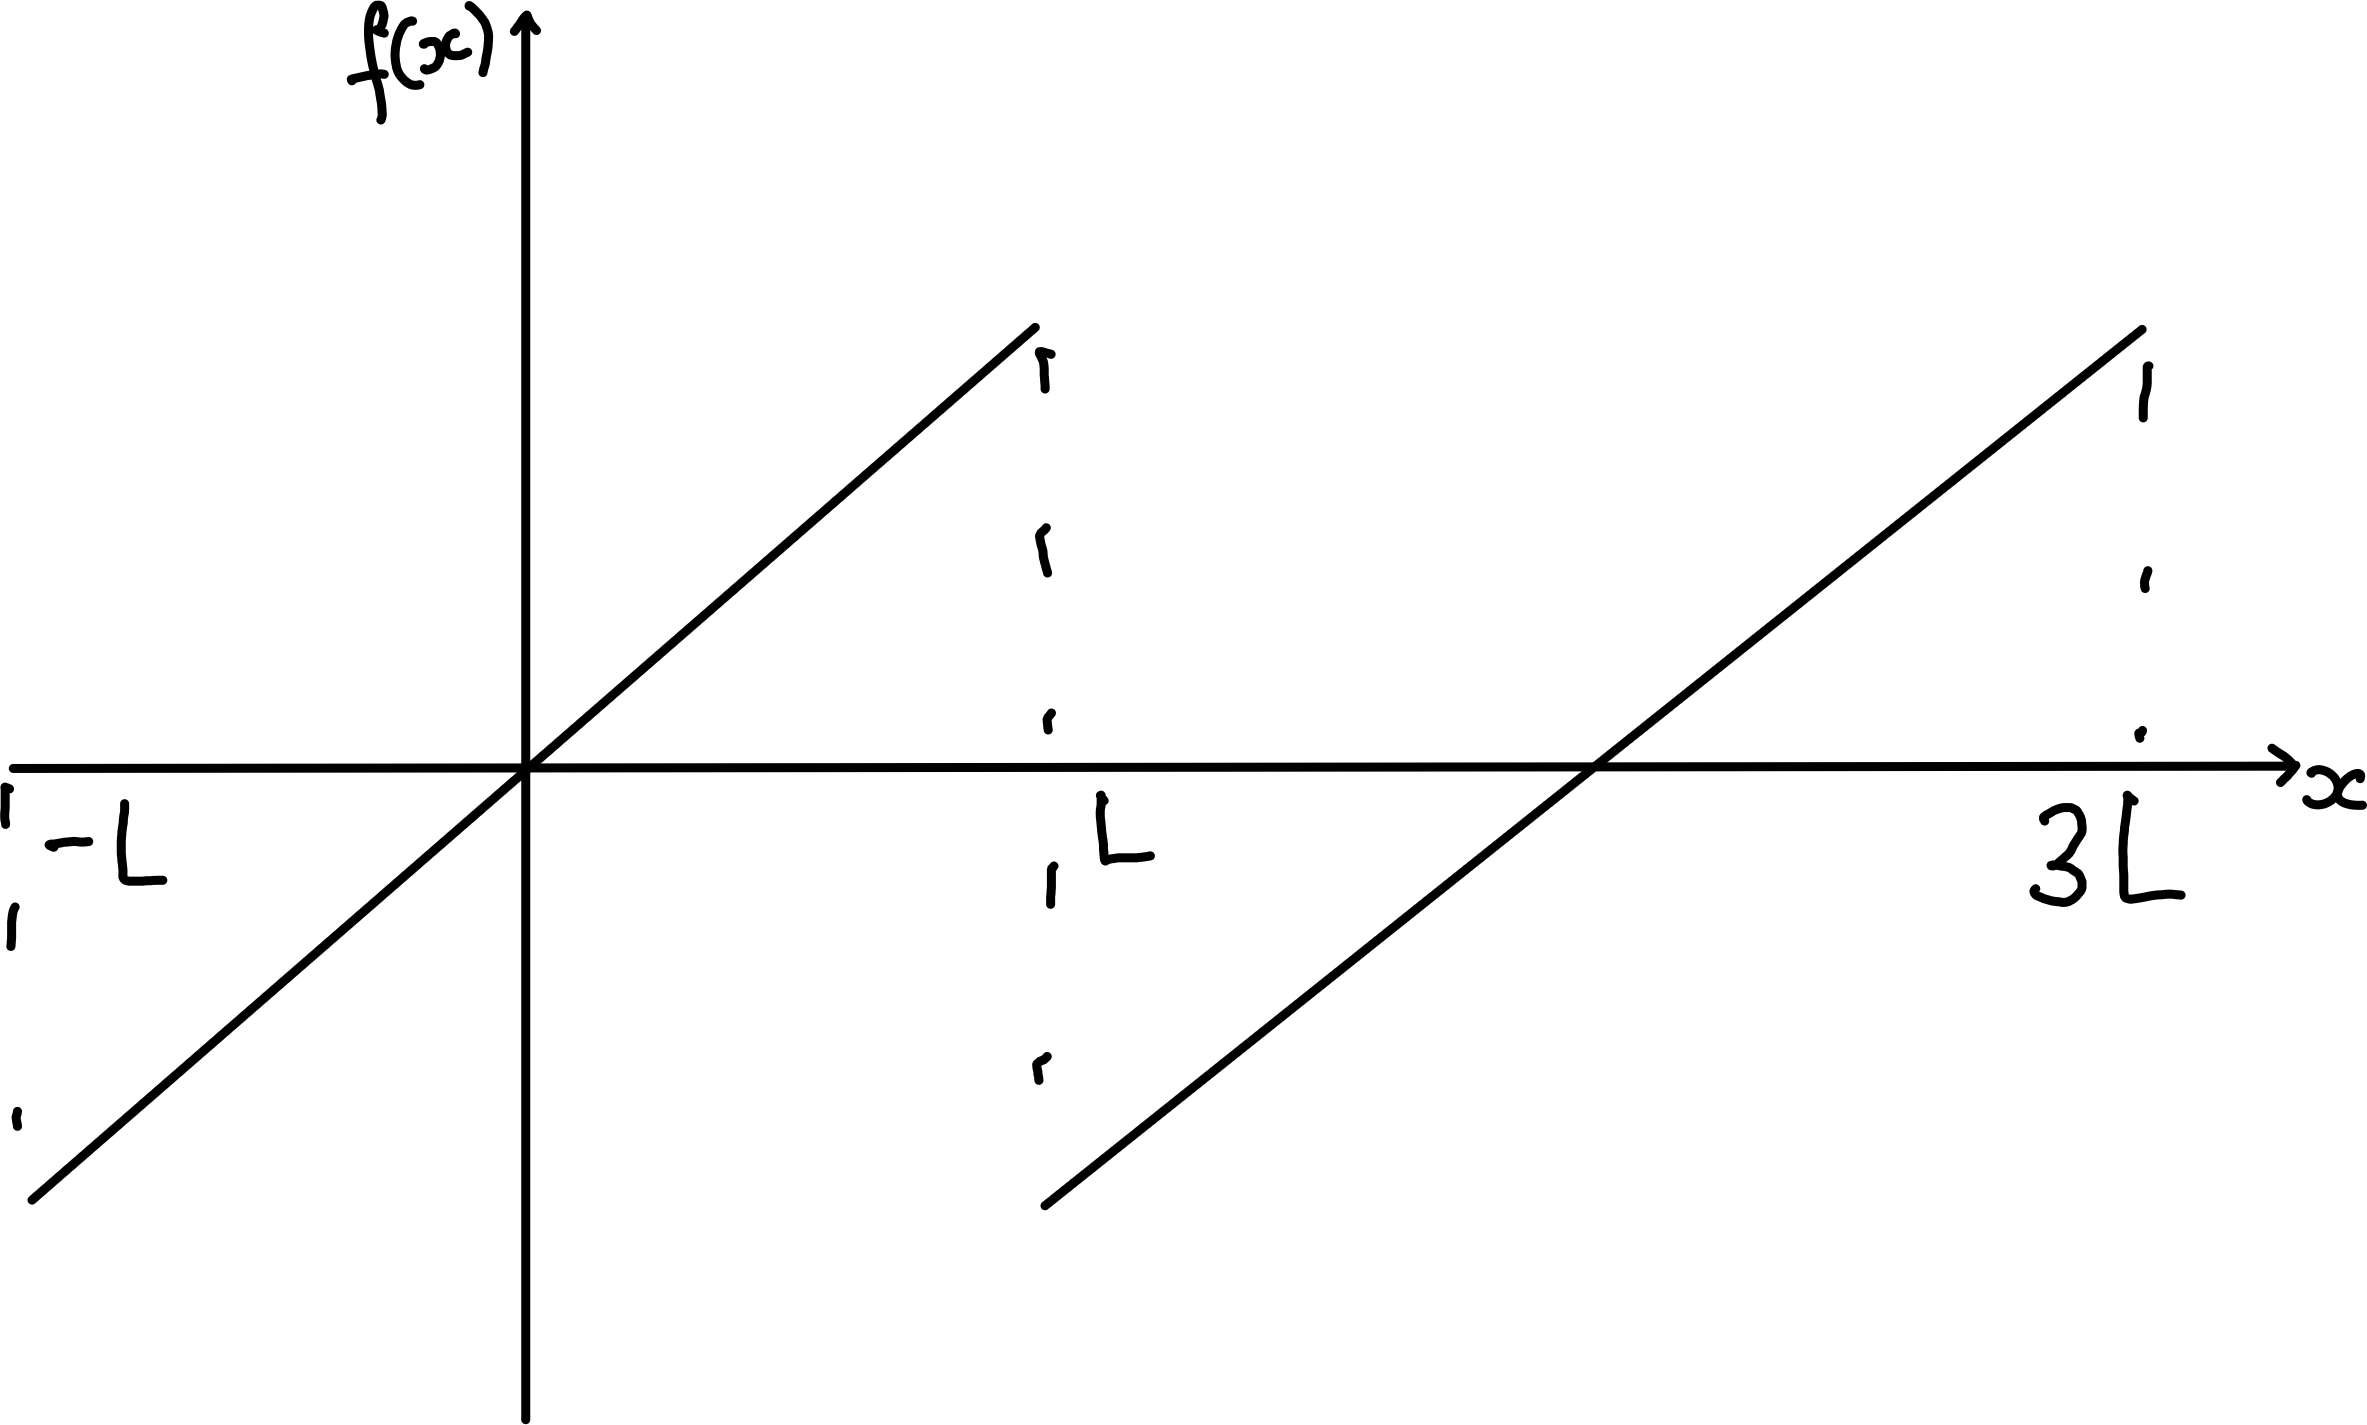
\includegraphics[height=5cm]{01-sawtooth} \par}
    Here,
    $a_n = \frac{1}{L} \int_{-L}^L x \cos \frac{n\pi x}{L} \dd{x} = 0$ as $x$ odd and $cos$ is even.
    \begin{align*}
        b_n &= \frac{1}{L} \int_{-L}^L x \sin \frac{n\pi x}{L} \dd{x} \\
        &= \frac{2}{L} \int_0^L x \sin \frac{n\pi x}{L} \dd{x} \text{ as the function we are integrating is even} \\
        &= \frac{-2}{n\pi} \qty[x \cos \frac{n\pi x}{L}]_0^L + \frac{2}{n\pi} \int_0^L \cos \frac{n \pi x}{L} \dd{x} \\
        &= \frac{-2L}{n\pi} \cos n \pi + \frac{2L}{(n\pi)^2} \sin n \pi \\
        &= \frac{2L}{n\pi} (-1)^{n+1}
    \end{align*}
    So the sawtooth FS is
    \begin{align} \label{eq:1.6}
        f(x) &= \frac{2L}{\pi} \sum_{n=1}^{\infty} \frac{(-1)^{n+1}}{n} \sin \frac{n \pi x}{L} \\
        &= \frac{2L}{\pi} \left( \sin \frac{\pi x}{L} - \frac{1}{2} \sin \frac{2 \pi x}{L} + \frac{1}{3} \sin \frac{3 \pi x}{L} + \dots \right) \notag
    \end{align} 
    which is slowly convergent.
    {\par \centering 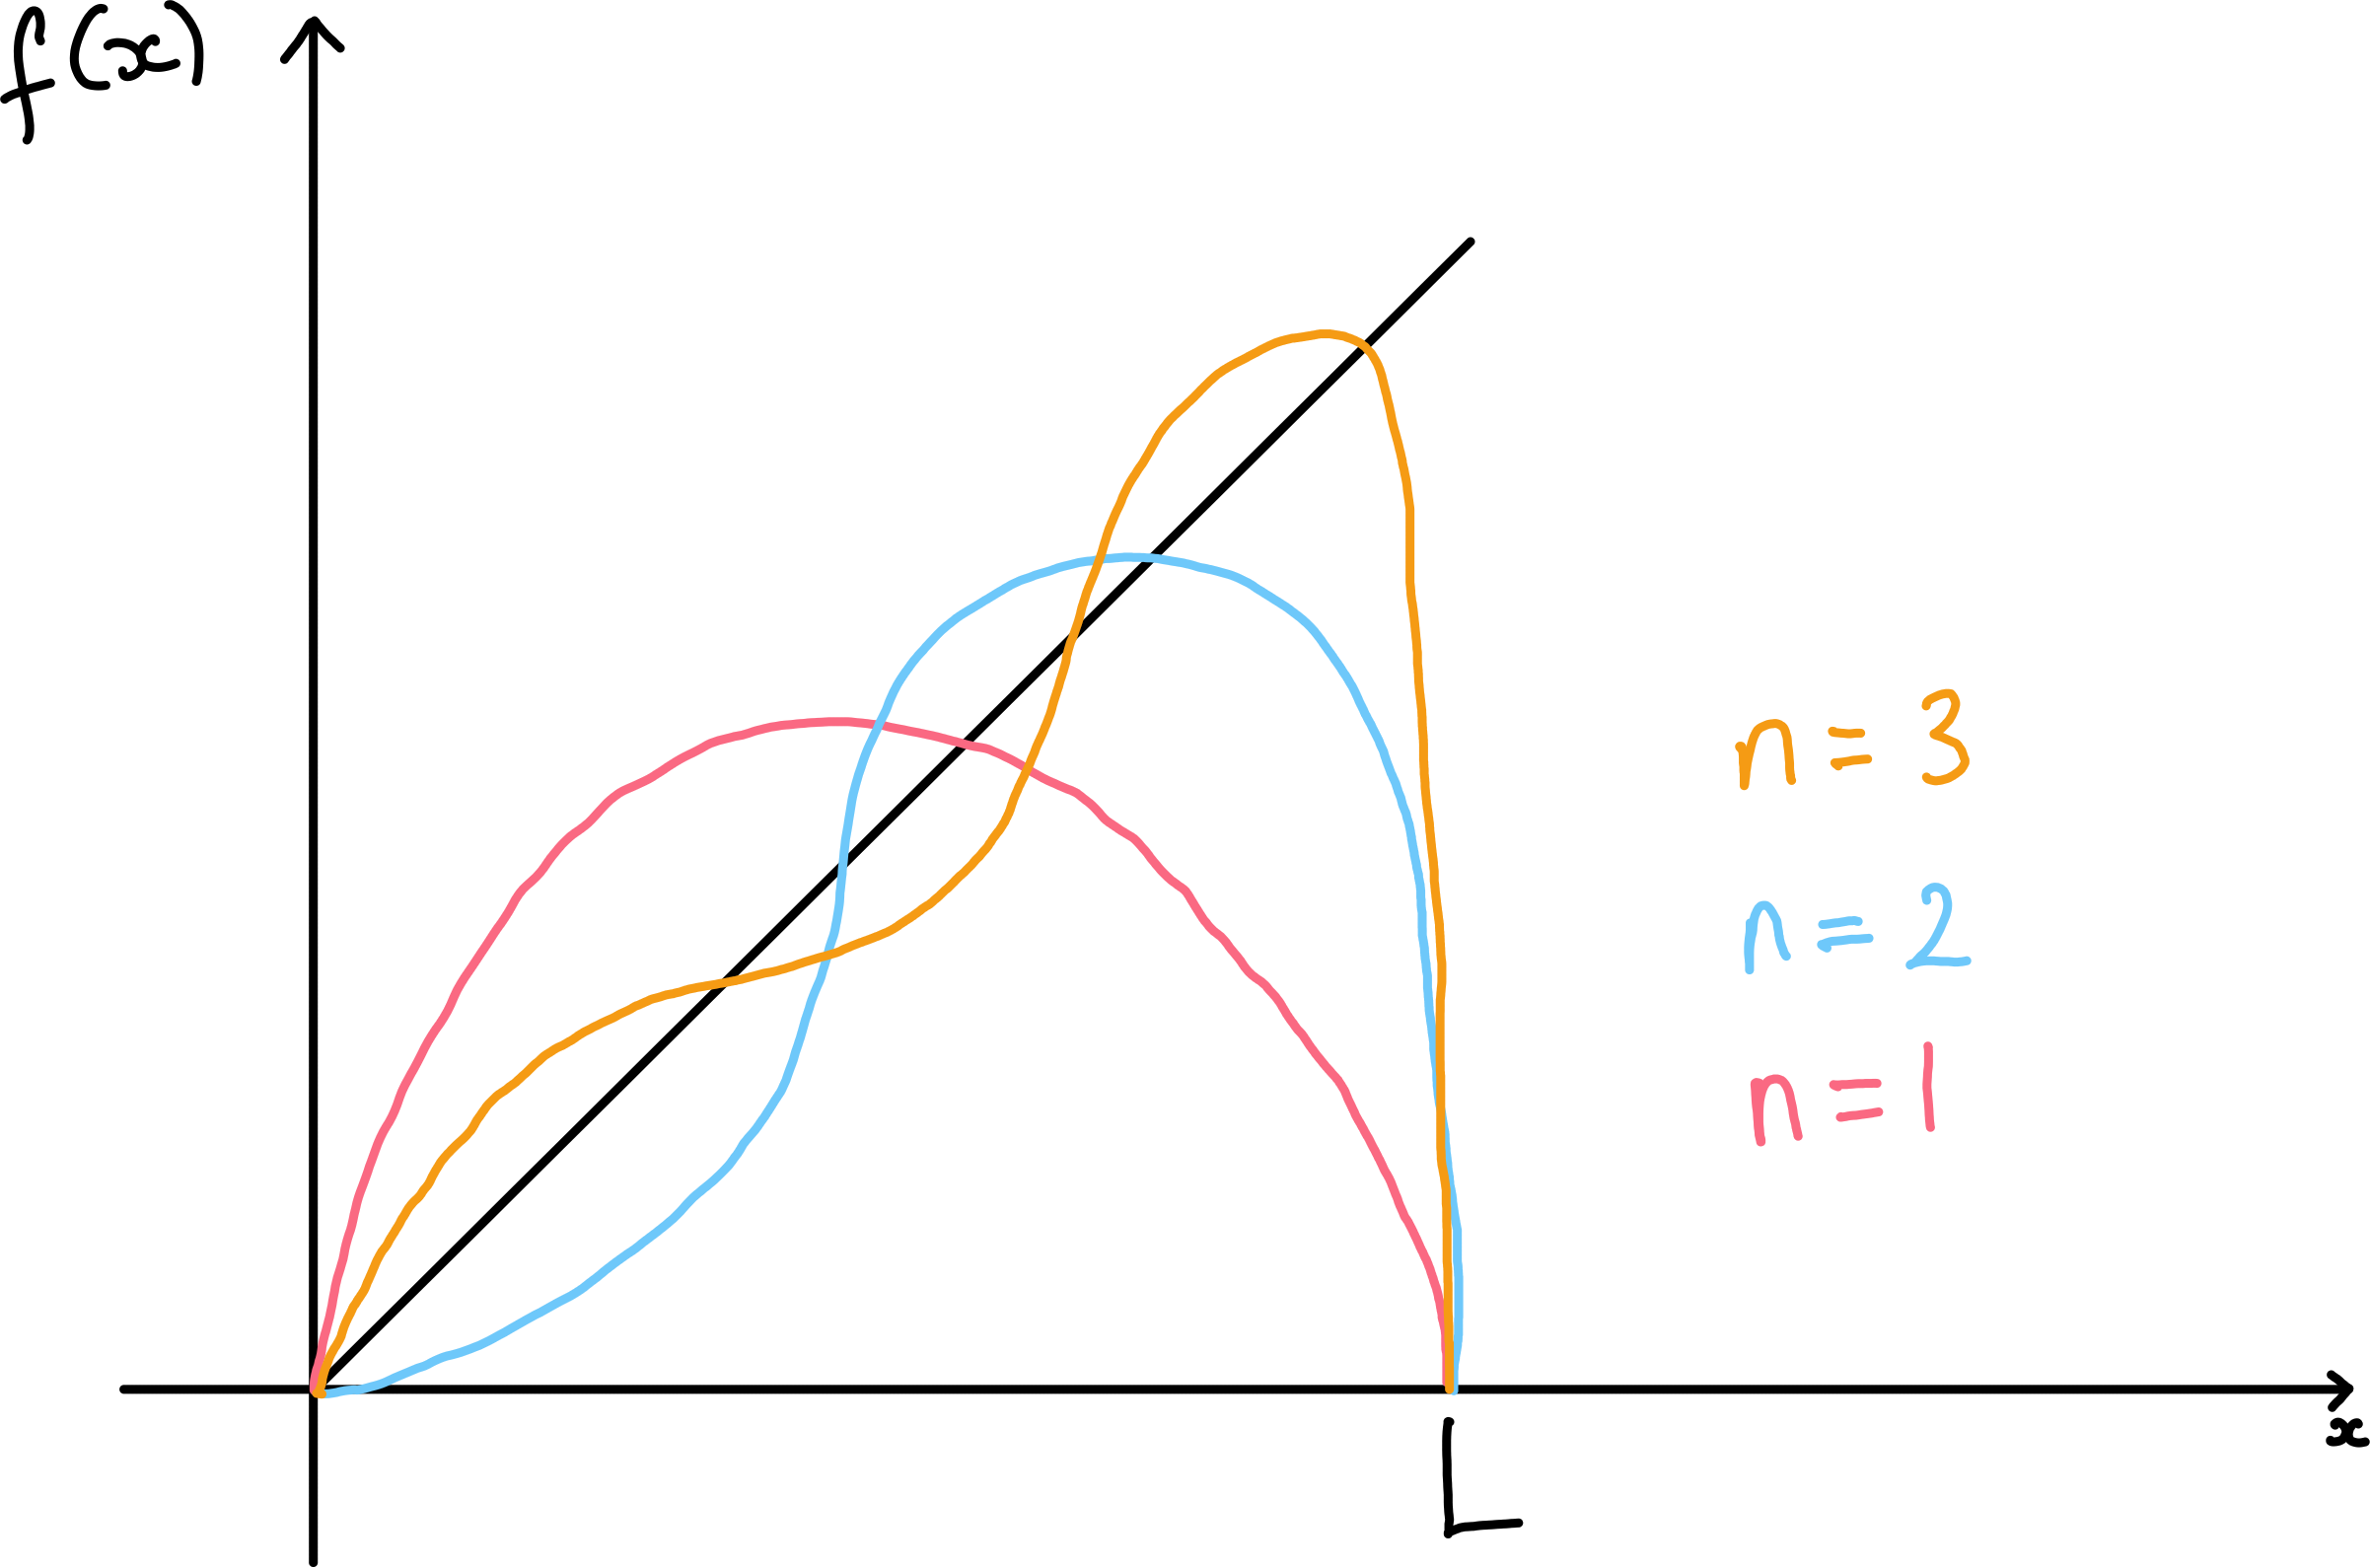
\includegraphics[height=5cm]{01-sawtooth2} \par}
\end{example}

\begin{note} As $n \to \infty$
    \begin{enumerate}
        \item FS approx improves (convergent when cts)
        \item $\text{FS} \to 0$ at $x = L$ i.e. midpoint of discontinuity
        \item FS has a persistent overshoot at $x = L$ (approx 9\% knows as Gibbs phenomenon, see Sheet 1, Q5).
    \end{enumerate} 
\end{note} 

\subsection{Dirichlet conditions}
The Dirichlet conditions are sufficiency conditions for a ``well-behaved'' function, that will imply the existence of a unique Fourier series.
\begin{theorem}
    If $f(x)$ is a bounded periodic function of period $2L$ with a finite number of minima, maxima and discontinuities in $[0, 2L)$, then the Fourier series converges to $f$ at all points at which $f$ is continuous, and at discontinuities the series converges to the midpoint.
\end{theorem}
\begin{note} \
    \begin{enumerate}
        \item These are some relatively weak conditions for convergence, compared to Taylor series.
            However, this definition still eliminates pathological functions such as $\frac{1}{x}$, $\sin \frac{1}{x}$, $\mathbbm 1 (\mathbb Q)$ and so on.
        \item \color{red}The converse is not true\color{black}; for example, $\sin \frac{1}{x}$ does in fact have a Fourier series.
        \item The proof is difficult and will not be given.
    \end{enumerate}
\end{note}

\noindent The rate of convergence of the Fourier series depends on the smoothness of the function.
\begin{theorem}
    If $f(x)$ has continuous derivatives up to a $p$th derivative which is discontinuous, then the Fourier series converges with order $O(n^{-(p+1)})$ as $n \to \infty$.
\end{theorem}
\begin{example}[$p = 0$]
    Consider the square wave (Sheet 1, Q5)
    \begin{align*}
        f(x) = \begin{cases}
            1  & 0 \leq x < 1  \\
            -1 & -1 \leq x < 0
        \end{cases}
    \end{align*}
    {\par \centering 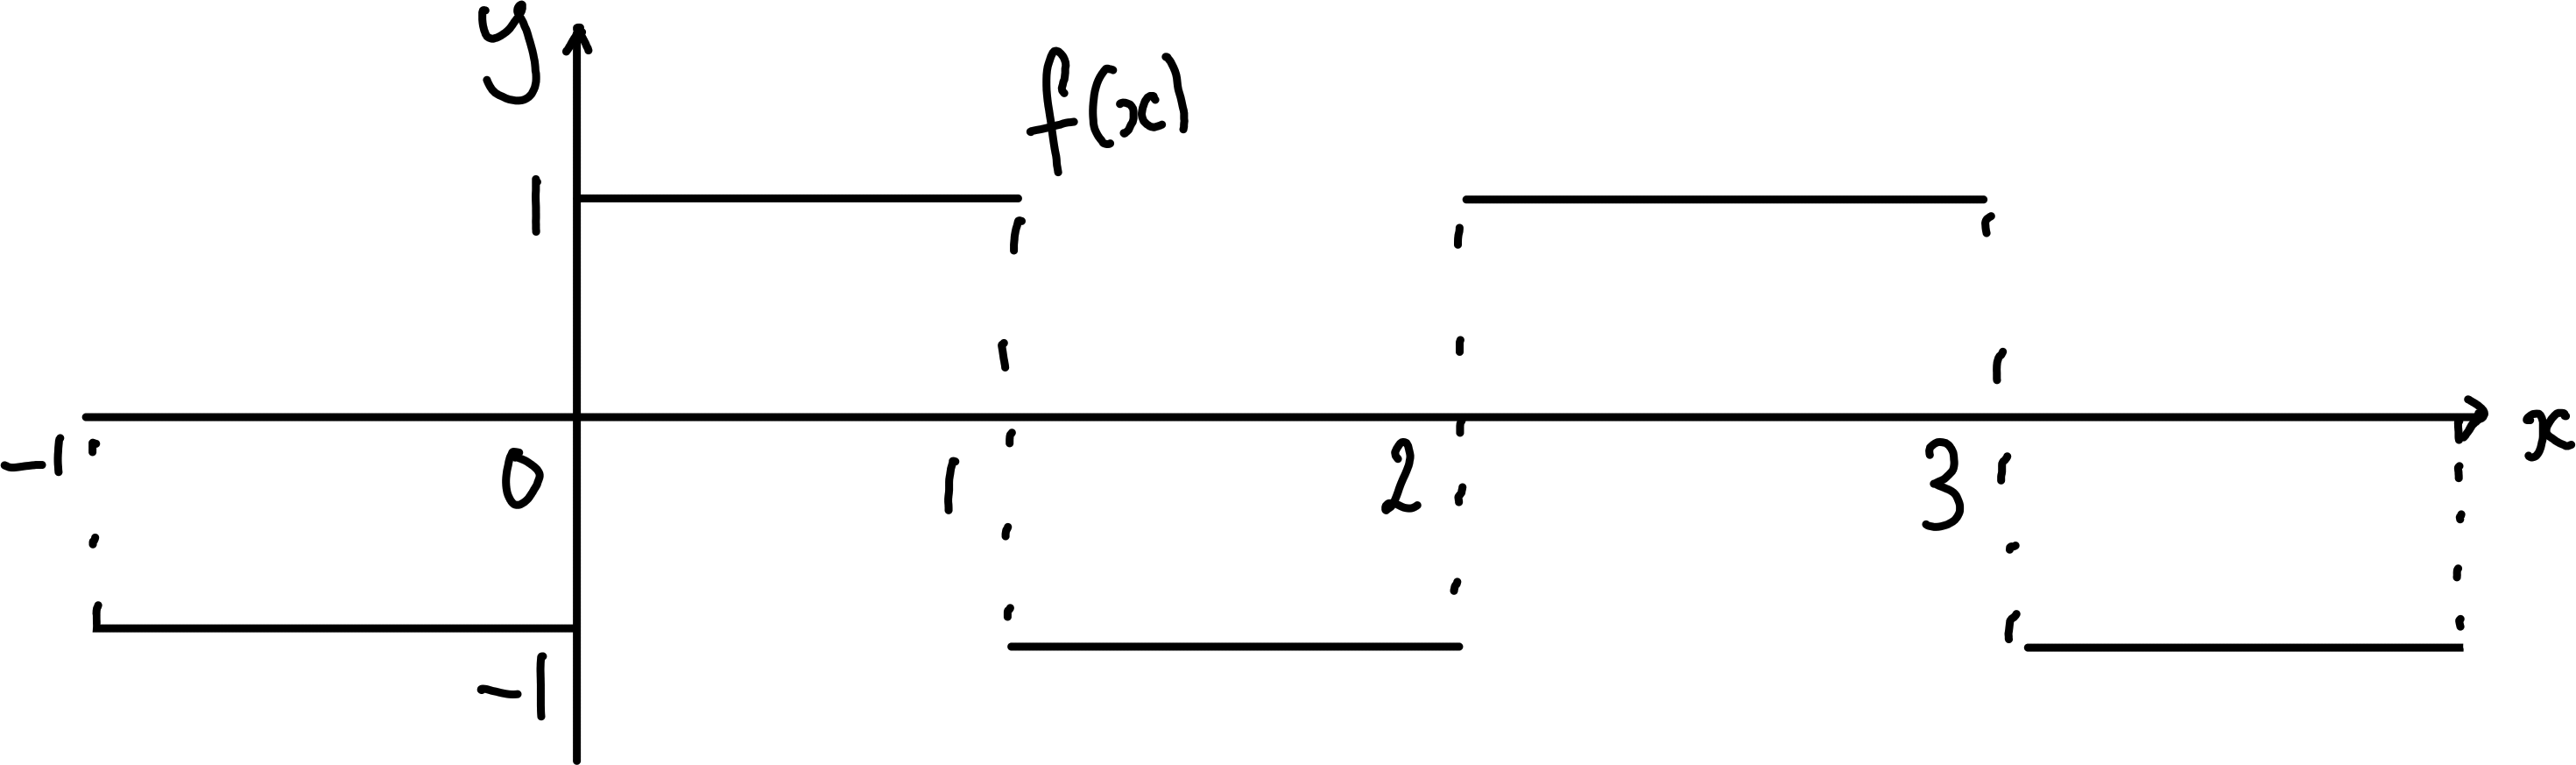
\includegraphics[height=5cm]{01-squarewave} \par}
    Then the Fourier series is
    \begin{align} \label{eq:1.7}
        f(x) = 4 \sum_{m=1}^\infty \frac{\sin (2m-1)\pi x}{(2m-1)\pi}
    \end{align}
\end{example}

\begin{example}[$p = 1$]
    Consider the general `see-saw' wave, defined by
    \begin{align*}
        f(x) = \begin{cases}
            x(1 - \xi) & 0 \leq x < \xi \\
            \xi(1 - x) & \xi \leq x < 1
        \end{cases}
    \end{align*}
    and defined as an odd function for $-1 \leq x < 0$.
    The Fourier series is\footnote{This is an important exercise you should do at home.}
    \begin{align} \label{eq:1.8}
        f(x) = 2 \sum_{m=1}^\infty \frac{\sin n\pi \xi \sin n\pi x}{(n \pi)^2}
    \end{align}
    
    {\par \centering 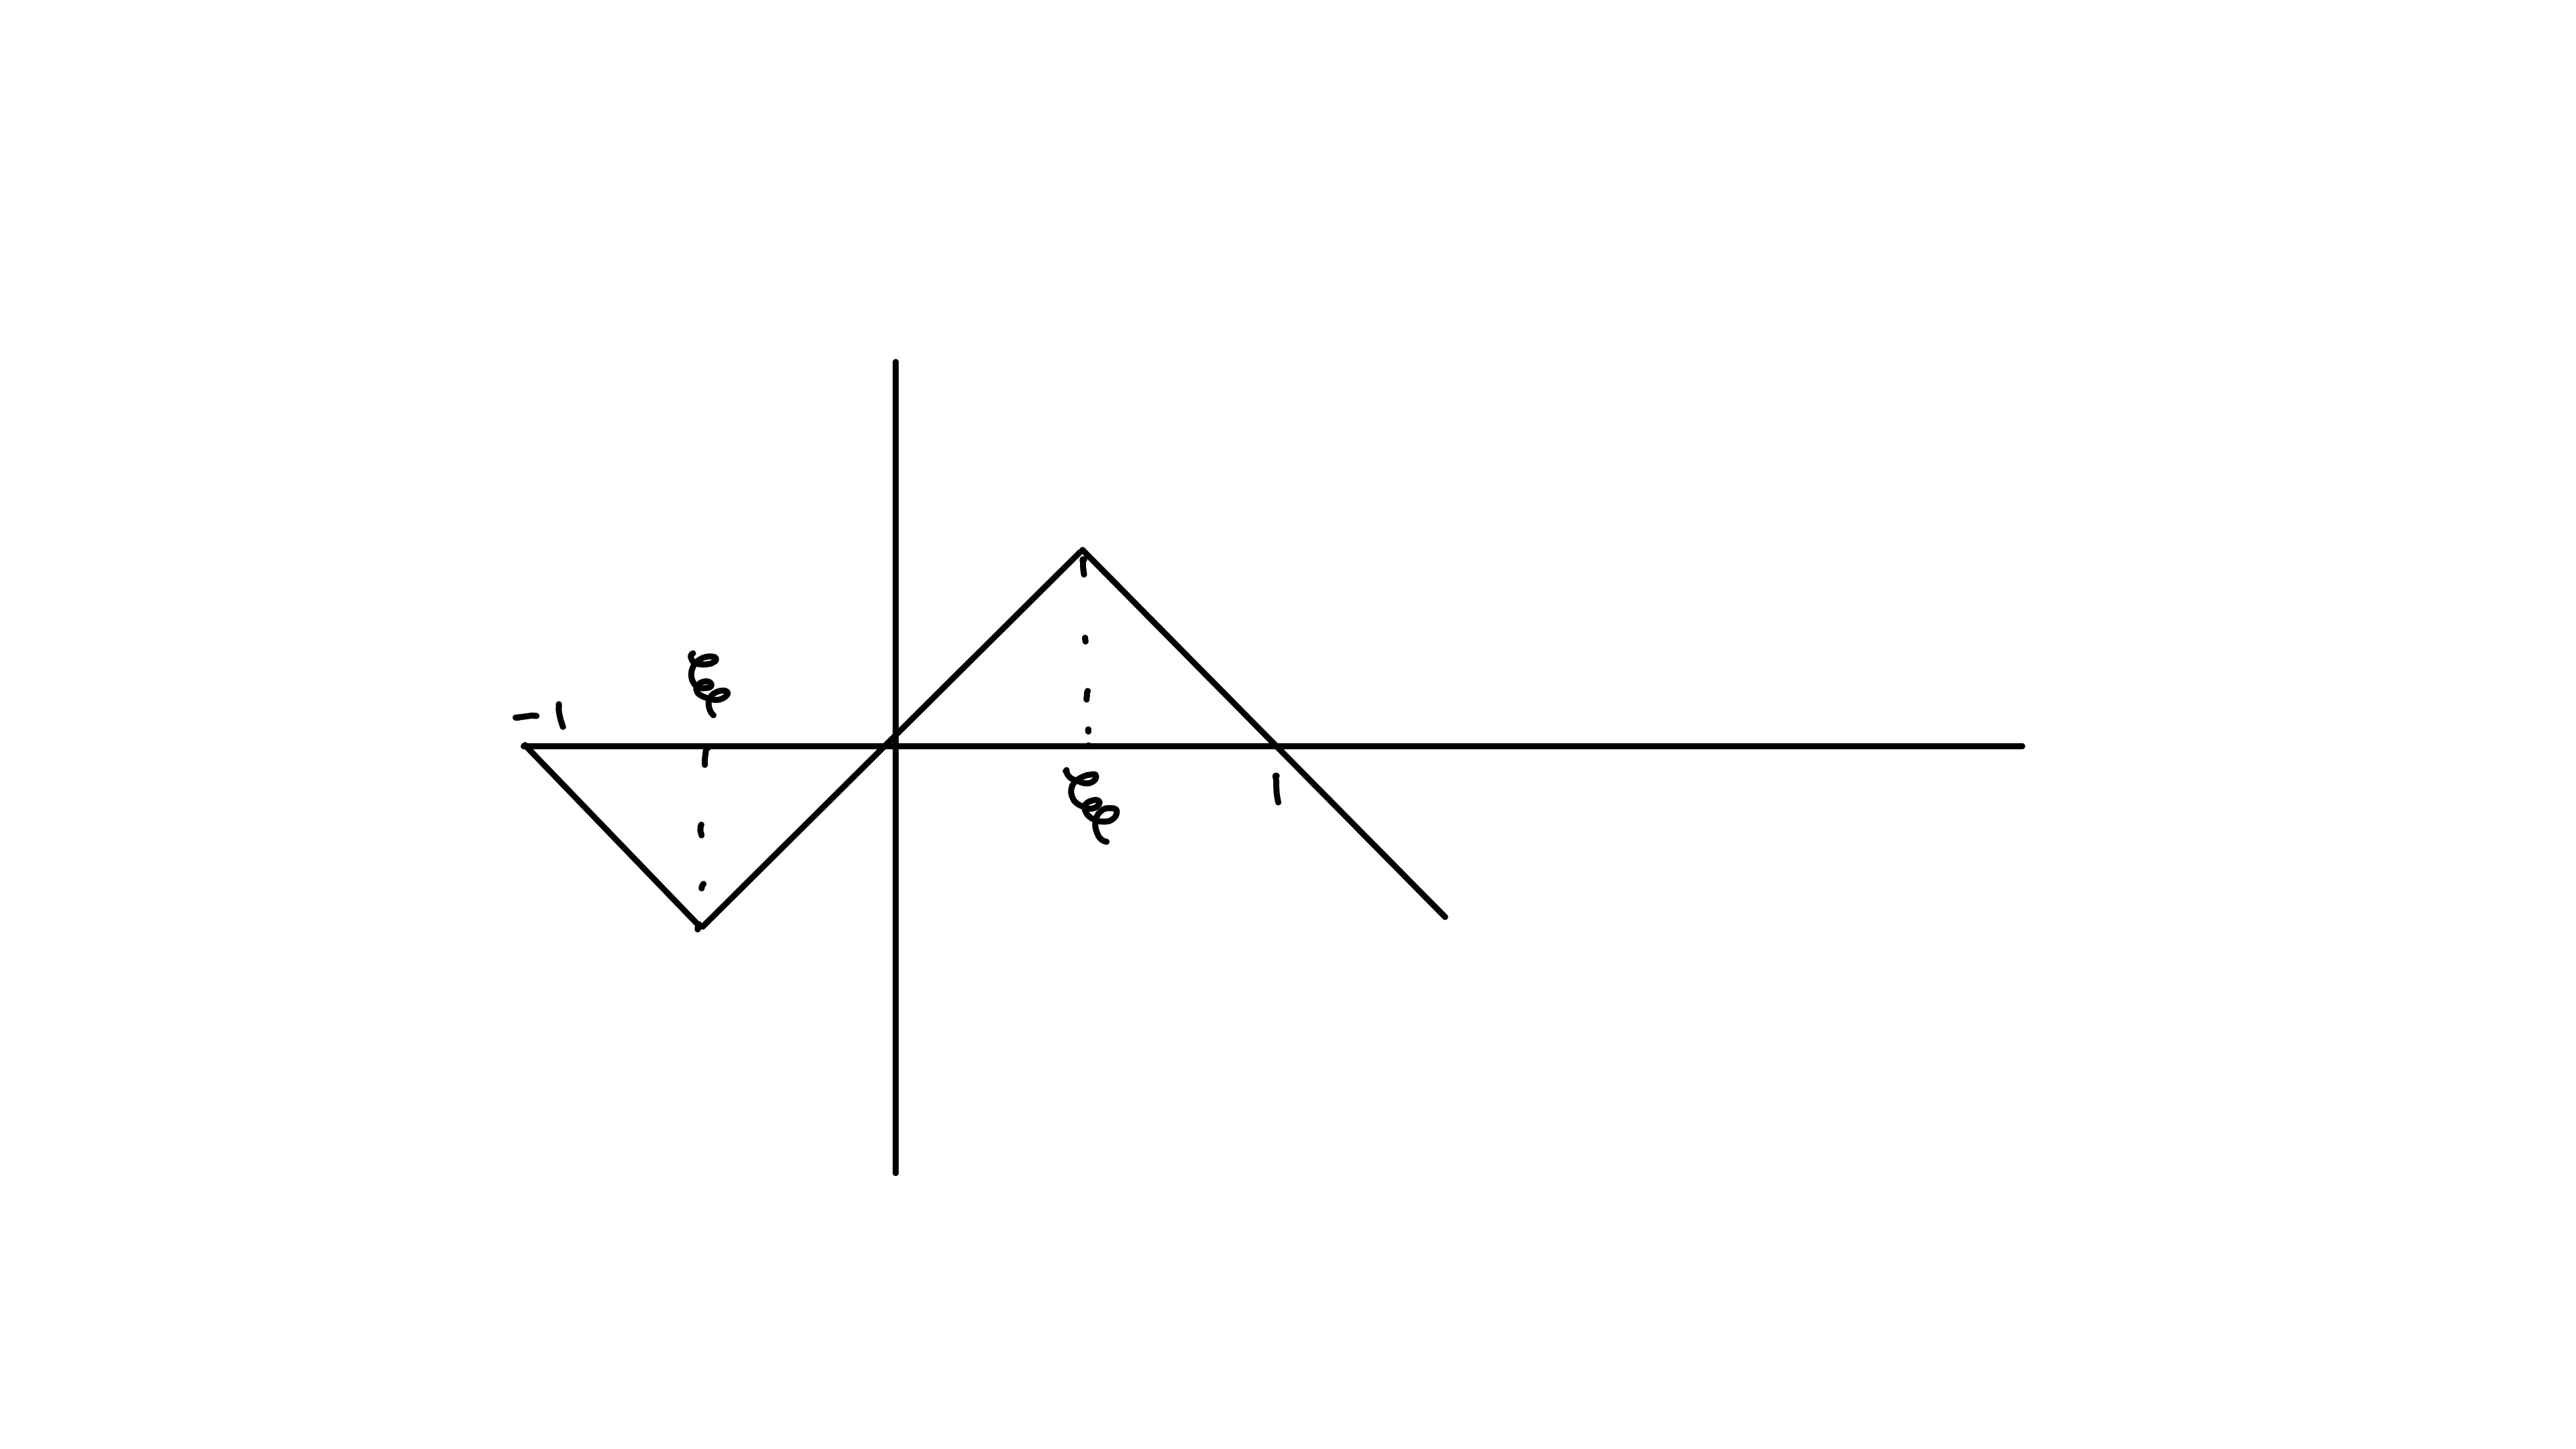
\includegraphics[height=5cm]{01-seesaw} \par}

    For instance, if $\xi = \frac{1}{2}$, we can show that
    \begin{align*}
        f(x) = 2 \sum_{m=1}^\infty (-1)^{m+1} \frac{\sin (2m-1)\pi x}{((2m-1)\pi)^2}
    \end{align*}
\end{example}
\begin{example}[$p = 2$]
    Let
    \begin{align*}
        f(x) = \frac{1}{2} x(1-x)
    \end{align*}
    for $0 \leq x < 1$, and defined as an odd function for $-1 \leq x < 0$.
    We can show that
    \begin{align} \label{eq:1.9}
        f(x) = 4\sum_{n=1}^\infty \frac{\sin(2m - 1)\pi x}{((2m-1)\pi)^3}
    \end{align}
    {\par \centering 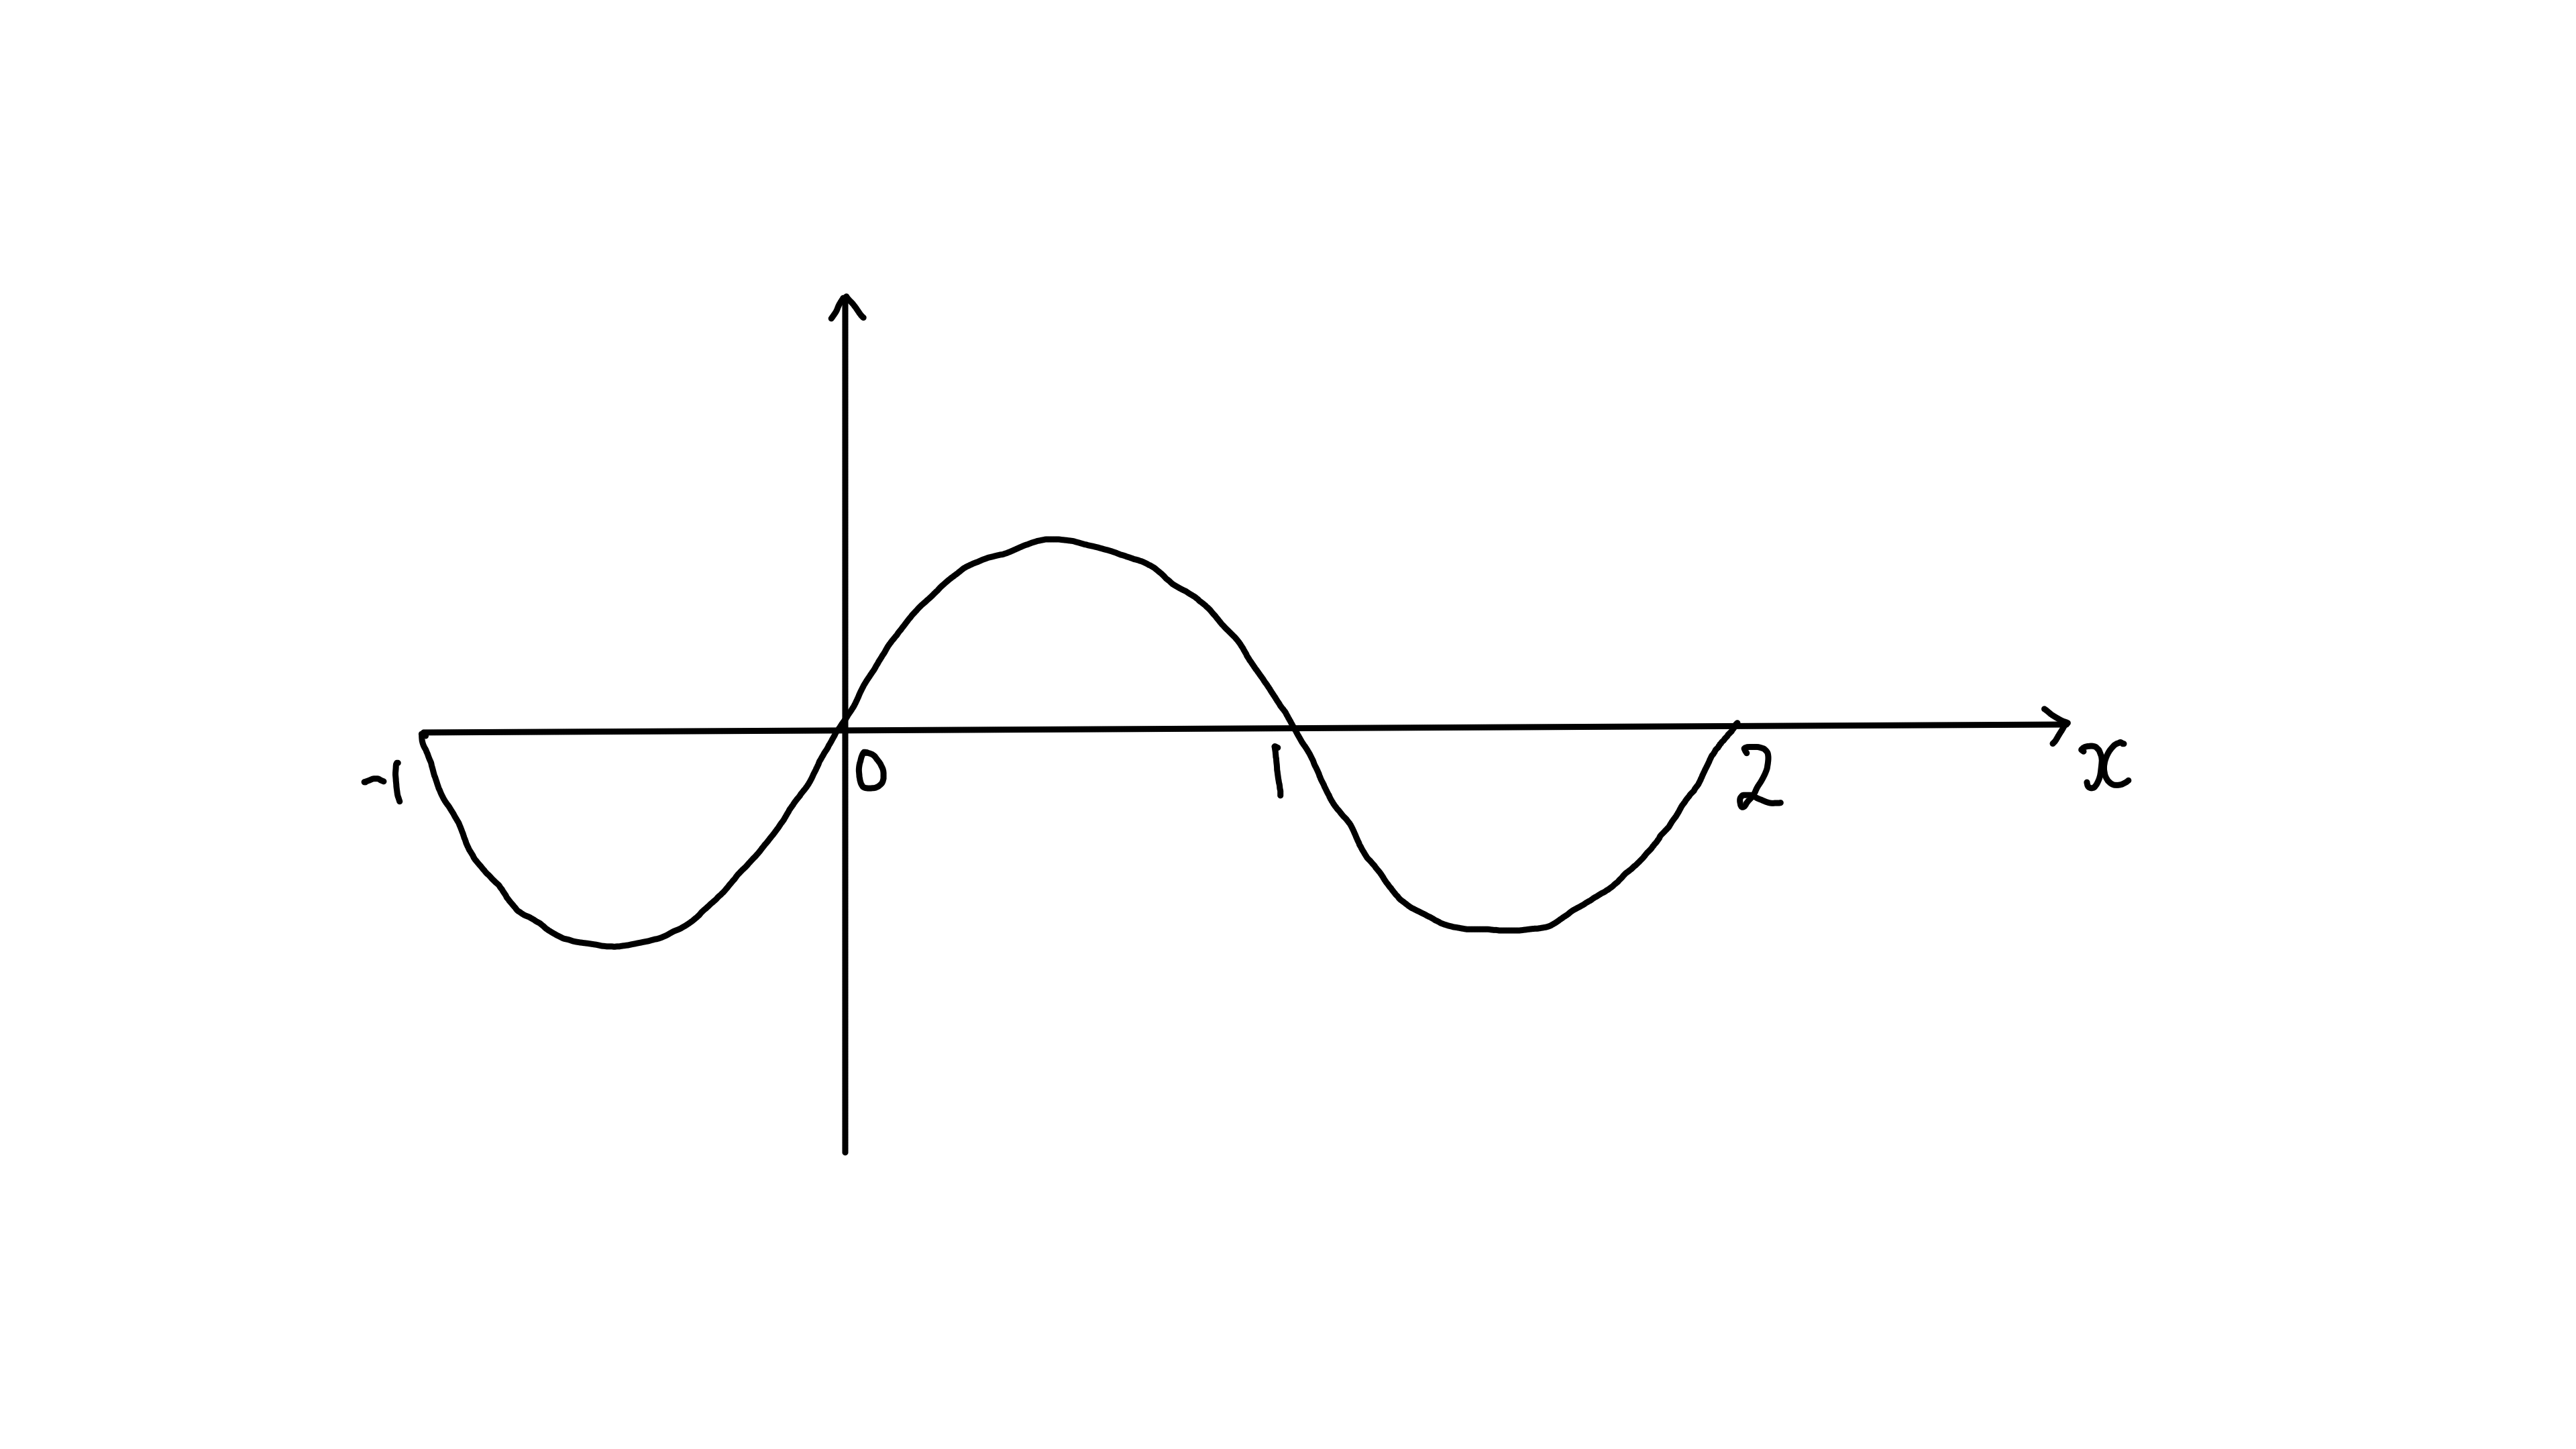
\includegraphics[height=5cm]{01-p2} \par}
\end{example}
\begin{example}[$p = 3$]
    Consider\footnote{Sheet 1, Q1}
    \begin{align*}
        f(x) = (1-x^2)^2
    \end{align*}
    with Fourier series
    \begin{align*}
        a_n = O\qty(\frac{1}{n^4})
    \end{align*}
\end{example}

\subsection{Integration of FS}
It is always valid to take the integral of a Fourier series term by term.
Defining $F(x) = \int_{-L}^x f(x) \dd{x}$, we can show that $F$ satisfies the Dirichlet conditions if $f$ does.
For instance, a jump discontinuity becomes continuous in the integral.

\subsection{Differentiation}
Differentiating term by term is not always valid.
For example, consider the square wave above:
\begin{align*}
    f(x) \stackrel{?}{=} 4 \sum_{m=1}^\infty \cos (2m-1)\pi x
\end{align*}
which is an unbounded series (consider $x = 0$).
\begin{theorem}
    If $f(x)$ is continuous and satisfies the Dirichlet conditions, and $f'(x)$ also satisfies the Dirichlet conditions, then $f'(x)$ can be found term by term by differentiating the Fourier series of $f(x)$.
\end{theorem}
\begin{example}
    We can differentiate the see-saw function, \cref{eq:1.8}, with $\xi = \frac{1}{2}$, even though the derivative is not continuous.
    The result is an offset square wave, or by mapping $x \mapsto x + \frac{1}{2}$ we recover the original square wave, \cref{eq:1.7}.
\end{example}

\subsection{Parseval's theorem}
Parseval's theorem relates the integral of the square of a function with the sum of the squares of the function's Fourier series coefficients.
\begin{theorem}[Parseval's theorem]
    Suppose $f$ has Fourier coefficients $a_i, b_i$.
    Then
    \begin{align}
        \int_0^{2L} [f(x)]^2 \dd{x} & = \int_0^{2L} \qty[ \frac{1}{2}a_0 + \sum_{n=1}^\infty a_n \cos \frac{n \pi x}{L} + \sum_{n=1}^\infty b_n \sin \frac{n\pi x}{L} ]^2 \dd{x} \notag \\
        \intertext{We can remove cross terms, since the basis functions are orthogonal. \cref{eq:1.1,eq:1.2,eq:1.3}}
        & = \int_0^{2L} \qty[ \frac{1}{4} a_0^2 + \sum_{n=1}^\infty a_n^2 \cos^2 \frac{n\pi x}{L} + \sum_{n=1}^\infty b_n^2 \sin^2 \frac{n\pi x}{L} ] \dd{x} \notag \\
        & = L \qty[ \frac{1}{2} a_0^2 + \sum_{n=1}^\infty (a_n^2 + b_n^2) ] \label{eq:1.10}
    \end{align}
\end{theorem}
\noindent This is also called the \textit{completeness relation}: the left hand side is greater than or equal to the right hand side if any of the basis functions are missing.
\begin{example}
    Let us apply Parseval's theorem to the sawtooth wave with FS \cref{eq:1.6}.
    \begin{align*}
        \int_{-L}^L [f(x)]^2 \dd{x} = \int_{-L}^L x^2 \dd{x} = \frac{2}{3}L^3
    \end{align*}
    The right hand side gives
    \begin{align*}
        L \sum_{n=1}^\infty \frac{4L^2}{n^2 \pi^2} = \frac{4 L^3}{\pi^2} \sum_{n=1}^\infty \frac{1}{n^2}
    \end{align*}
    Parseval's theorem then implies\footnote{Sheet 1, Q3}
    \begin{align*}
        \sum_{n=1}^\infty \frac{1}{n^2} = \frac{\pi^2}{6}
    \end{align*}
\end{example}
\begin{note}
    Parseval's theorem for functions $\inner{f, f} = \norm{f}^2$ is equivalent to Pythagoras for vectors $\inner{v, v} = \norm{v}^2$.
\end{note} 

\subsection{Half-range series}
Consider $f(x)$ defined only on $0 \leq x < L$.
We can extend the range of $f$ to be the full range $-L \leq x < L$ in two simple ways:
\begin{enumerate}
    \item require $f$ to be odd, so $f(-x) = -f(x)$.
        Hence, $a_n = 0$ (as $\cos$ is even) and
        \begin{align} \label{eq:1.11}
            b_n = \frac{2}{L} \int_0^L f(x) \sin \frac{n \pi x}{L} \dd{x}
        \end{align}
        So
        \begin{align*}
            f(x) = \sum_{n=1}^\infty b_n \sin \frac{n\pi x}{L}
        \end{align*}
        which is called a Fourier sine series.
    \item require $f$ to be even, so $f(-x) = f(x)$.
        In this case, $b_n = 0$ and
        \begin{align} \label{eq:1.12}
            a_n = \frac{2}{L} \int_0^L f(x) \cos \frac{n \pi x}{L} \dd{x}
        \end{align}
        and so
        \begin{align*}
            f(x) = \frac{1}{2}a_0 + \sum_{n=1}^\infty a_n \cos \frac{n\pi x}{L}
        \end{align*}
        which is a Fourier cosine series.
\end{enumerate}

\subsection{Complex representation of Fourier series}
Recall that
\begin{align*}
    \cos \frac{n \pi x}{L} &= \frac{1}{2}\qty(e^{i n \pi x / L} + e^{-i n \pi x / L}); \\
    \sin \frac{n \pi x}{L} &= \frac{1}{2i}\qty(e^{i n \pi x / L} - e^{-i n \pi x / L})
\end{align*}
Therefore, a Fourier series can be written as
\begin{align}
    f(x) &= \frac{1}{2} a_0 + \frac{1}{2} \sum_{n=1}^\infty \qty[ (a_n - i b_n) e^{i n \pi x / L} + (a_n + i b_n) e^{-i n \pi x / L} ] \notag \\
    &= \sum_{m=-\infty}^\infty c_m e^{i m \pi x / L} \label{eq:1.13}
\end{align}
where for $m > 0$ we have $m=n, c_m = \frac{1}{2}(a_n - ib_n)$, and for $m < 0$ we have $n = -m, c_m = \frac{1}{2}(a_{-m} + ib_{-m})$, and where $m = 0$ we have $c_0 = \frac{1}{2} a_0$.
In particular,
\begin{align} \label{eq:1.14}
    c_m = \frac{1}{2L} \int_{-L}^L f(x) e^{-i m \pi x / L} \dd{x}
\end{align}
where the negative sign comes from the complex conjugate.
This is because, for complex-valued $f, g$, we have
\begin{definition}[Complex inner product] ~\vspace*{-1.5\baselineskip}
    \begin{align*}
        \inner{f,g} = \int_{-L}^L f^\star\footnote{$f^\star$ is the complex conjugate of $f$.} g \dd{x}
    \end{align*}
\end{definition} 
The orthogonality conditions are
\begin{align} \label{eq:1.15}
    \int_{-L}^L e^{-i m \pi x / L} e^{i n \pi x / L} \dd{x} = 2L \delta_{mn}
\end{align}
Parseval's theorem now states
\begin{align*}
    \int_{-L}^L f^\star(x) f(x) \dd{x} = \int_{-L}^L \abs{f(x)}^2 \dd{x} = 2L \sum_{m=-\infty}^\infty \abs{c_m}^2
\end{align*}

\subsection{Self-adjoint matrices}
\textit{Much of this section is a recap of IA Vectors and Matrices.}
Suppose that $u, v \in \mathbb C^N$ with inner product
\begin{align} \label{eq:1.16}
    \inner{u,v} = u^\dagger v
\end{align}
\begin{definition}[Hermitian matrix] 
    The $N \times N$ matrix $A$ is \textit{self-adjoint}, or \textit{Hermitian}, if
    \begin{align*}
        \forall u,v \in \mathbb C^N, \inner{Au, v} = \inner{u, Av} \iff A^\dagger = A
    \end{align*}
\end{definition} 
The eigenvalues $\lambda_n$ and eigenvectors $v_n$ satisfy
\begin{align} \label{eq:1.17}
    A v_n = \lambda_n v_n
\end{align}
They have the following properties:
\begin{enumerate}
    \item $\lambda_n^\star = \lambda_n$;
    \item $\lambda_n \neq \lambda_m \implies \inner{ v_n, v_m } = 0$;
    \item we can create an orthonormal basis from the eigenvectors.
\end{enumerate}
Given $b \in \mathbb C^n$, we can solve for $x$ in the general matrix equation 
\begin{align}
    Ax = b \label{eq:1.18}
\end{align}
Express $b$ in terms of the eigenvector basis:
\begin{align*}
    b = \sum_{n=1}^N b_n v_n \notag
\end{align*}
We seek a solution of the form
\begin{align*}
    x = \sum_{n=1}^N c_n v_n
\end{align*}
At this point, the $b_n$ are known and the $c_n$ are our target.
Substituting into the matrix equation \cref{eq:1.18}, orthogonality of basis vectors gives
\begin{align*}
    A \sum_{n=1}^N c_n v_n &= \sum_{n=1}^N b_n v_n \\
    \sum_{n=1}^N c_n \lambda_n v_n &= \sum_{n=1}^N b_n v_n
    \intertext{As the eigenvector basis is orthogonal we can equate coefficients}
    c_n \lambda_n &= b_n \\
    c_n &= \frac{b_n}{\lambda_n}
\end{align*}
Therefore,
\begin{align} \label{eq:1.19}
    x = \sum_{n=1}^N \frac{b_n}{\lambda_n} v_n
\end{align}
provided $\lambda_n \neq 0$, or equivalently, the matrix is invertible.

\subsection{Solving inhomogeneous ODEs with Fourier series} \label{sec:1.6}
We wish to find $y(x)$ given a driving/ source term $f(x)$ for the general differential equation
\begin{align} \label{eq:1.20}
    \mathcal L y \equiv -\dv[2]{y}{x} = f(x)
\end{align}
with boundary conditions $y(0) = y(L) = 0$.
The related eigenvalue problem is
\begin{align*}
    \mathcal L y_n = \lambda_n y_n,\quad y_n(0) = y_n(L) = 0
\end{align*}
which has solutions
\begin{align} \label{eq:1.21}
    y_n(x) = \sin \frac{n \pi x}{L},\ \lambda_n = \qty(\frac{n\pi}{L})^2
\end{align}
We can show that this is a self-adjoint linear operator\footnote{https://math.stackexchange.com/questions/4356100/why-is-the-second-derivative-operator-self-adjoint} with orthogonal eigenfunctions.
We seek solutions of the form of a half-range sine series.
Consider
\begin{align*}
    y(x) = \sum_{n=1}^\infty c_n \sin\frac{n \pi x}{L}
\end{align*}
The right hand side is
\begin{align*}
    f(x) = \sum_{n=1}^\infty b_n \sin \frac{n \pi x}{L}
\end{align*}
We can find $b_n$ by
\begin{align*}
    b_n = \frac{2}{L} \int_0^L f(x) \sin \frac{n \pi x}{L} \dd{x}
\end{align*}
Substituting into \cref{eq:1.20}, we have
\begin{align*}
    \mathcal L y = -\dv[2]{x} \qty(\sum_n c_n \sin \frac{n \pi x}{L}) &= \sum_n c_n \qty(\frac{n\pi}{L})^2 \sin \frac{n \pi x}{L} \\
    \text{So } \sum_n c_n \qty(\frac{n\pi}{L})^2 \sin \frac{n \pi x}{L} &= \sum_n b_n \sin \frac{n \pi x}{L}
\end{align*}
By orthogonality \cref{eq:1.1},
\begin{align*}
    c_n \qty(\frac{n \pi}{L})^2 = b_n \implies c_n = \qty(\frac{L}{n \pi})^2 b_n
\end{align*}
Therefore the solution is
\begin{align} \label{eq:1.22}
    y(x) = \sum_n \qty(\frac{L}{n \pi})^2 b_n \sin \frac{n \pi x}{L} = \sum_n \frac{b_n}{\lambda_n} y_n
\end{align}
which is equivalent to the solution we found for self-adjoint matrices for which the eigenvalues and eigenvectors are known.
\begin{example}[Odd square wave]
    Consider an odd square wave with $L = 1$, so $f(x) = 1$ from $0 \leq x < 1$.
    \begin{align*}
        f(x) = 4 \sum_m \frac{\sin(2m-1)\pi x}{(2m-1)\pi} \text{ by \cref{eq:1.7}}
    \end{align*}
    Then the solution to $\mathcal L y = f$ \cref{eq:1.22} should be (with odd $n = 2m-1$)
    \begin{align*}
        y(x) = \sum_n \frac{b_n}{\lambda_n} y_n = 4 \sum_n \frac{\sin (2m-1) \pi x}{((2m - 1) \pi)^3}
    \end{align*}
    This is exactly the Fourier series for
    \begin{align*}
        y(x) = \frac{1}{2}x(1-x) \text{ by \cref{eq:1.9}}
    \end{align*}
    so this $y$ is the solution to the differential equation.
    We can in fact integrate $\mathcal L y = 1$ directly with the boundary conditions to verify the solution.
    We can also differentiate the Fourier series for $y$ twice to find the square wave.
\end{example}
    \section{Sturm-Liouville Theory}

\subsection{Review of second-order linear ODEs}
\textit{This section is a review of IA Differential Equations.}

We wish to solve a general inhomogeneous ODE, written
\begin{align} \label{eq:2.1}
    \mathcal L y \equiv \alpha(x) y'' + \beta(x) y' + \gamma(x) y = f(x)
\end{align}
The homogeneous version has $f(x) = 0$, so \begin{align} \label{eq:2.2}
    \mathcal{L}y = 0,
\end{align} which has two independent solutions $y_1, y_2$.
The general solution, also the complementary function for the inhomogeneous ODE, is 
\begin{align}
    y_c(x) = A y_1(x) + B y_2(x). \label{eq:2.3}
\end{align}

The inhomogeneous equation 
\begin{align}
    \mathcal L y = f(x) \label{eq:2.4}
\end{align} has a solution called the particular integral, denoted $y_p(x)$.
The general solution to this equation is then 
\begin{align} \label{eq:2.5}
    y(x) = y_p + y_c.
\end{align}

We need two boundary or initial conditions to find the particular solution to the differential equation.
Suppose $x \in [a,b]$.
We can create boundary conditions by defining $y(a), y(b)$, often called the Dirichlet conditions.
Alternatively, we can consider $y(a), y'(a)$, called the Neumann conditions.
We could also used some kind of mixed condition, for instance $y + ky'$.

Homogeneous boundary conditions are such that $y(a) = y(b) = 0$.
In this part of the course, homogeneous boundary conditions are often assumed.
Note that we can add a complementary function $y_c$ to the solution, for instance $\overline{y} = y + A y_1 + B y_2$ such that $\overline{y}(a) = \overline{y}(b) = 0$.
This would allow us to construct homogeneous boundary conditions even when they are not present \textit{a priori} in the problem.
We could also specify initial data, such as solving for $x \geq a$, given $y, y'$ at $x = a$.

To solve the inhomogeneous equation \cref{eq:2.1}, we want to use eigenfunction expansions (like FS \cref{eq:1.22}).
In order to do this, we must first solve the \underline{related} eigenvalue problem.
In this case, that is
\begin{align}
    \alpha(x) y'' + \beta(x) y' + \gamma(x) y = -\lambda \rho(x) y. \label{eq:2.6}
\end{align}
We must solve this equation with the same boundary conditions as the original problem.
This form of equation often arises as a result of applying a separation of variables, particularly for PDEs in several dimensions.

\subsection{Sturm-Liouville form}
\begin{definition}[Inner product]
    For two complex-valued functions $f, g$ on $[a,b]$, we define the inner product as
    \begin{align*}
        \inner{f,g} = \int_a^b f^\star(x) g(x) \dd{x}
    \end{align*} 
\end{definition} 
The eigenvalue problem \cref{eq:2.6} above greatly simplifies if $\mathcal L$ is \underline{self-adjoint}, that is, if it can be expressed in \underline{Sturm-Liouville form}:
\begin{align} \label{eq:2.7}
    \mathcal L y \equiv -(py')' + qy = \lambda w y.
\end{align}
$\lambda$ is an eigenvalue, and $w(x)$ is the \textit{weight function}, which must be non-negative $w(x) \geq 0 \ \forall \; x$.

\subsection{Converting to Sturm-Liouville form}
Multiply \cref{eq:2.6} by an integrating factor $F(x)$ to give
\begin{align*}
    F \alpha y'' + F \beta y' + F \gamma y &= -\lambda F \rho y \\
    \dv{x} \qty(F \alpha y') - F' \alpha y' - F \alpha' y' + F \beta y' + F \gamma y &= -\lambda F \rho y
\end{align*}
To eliminate the $y'$ term, we require $F'\alpha = F(\beta - \alpha')$.
Thus,
\begin{align}
    \frac{F'}{F} &= \frac{\beta - \alpha'}{\alpha} \notag \\
    \implies F &= \exp \int^x \frac{\beta - \alpha'}{\alpha} \dd{x} \label{eq:2.8}
\end{align}
and further,
\begin{align*}
    (F\alpha y')' + F \gamma y = - \lambda F \rho y
\end{align*}
hence
\begin{align*}
    p & = F \alpha \\
    q & = F \gamma \\
    w & = F \rho
\end{align*} in $\cref{eq:2.7}$ and $F(x) > 0$ hence $w > 0$.
\begin{example}
    Consider the Hermite equation for simple harmonic oscillator,
    \begin{align*}
        y'' - 2xy' + 2ny = 0
    \end{align*}
    In this case for \cref{eq:2.6} $\alpha = 1,\ \beta = -2x,\ \gamma = 0,\ \lambda p = 2n$.
    So by \cref{eq:2.8}
    \begin{align*}
        F = \exp \int^x \frac{-2x}{1} \dd{x} = e^{-x^2}
    \end{align*}
    Then the equation, in Sturm-Liouville form, is
    \begin{align}
        \mathcal L y \equiv -\qty(e^{-x^2} y')' = 2n e^{-x^2} y \label{eq:2.9}
    \end{align}
\end{example}

\subsection{Self-adjoint operators}
\begin{definition}[Self-adjoint operator]
    $\mathcal L$ is a self-adjoint operator on $[a,b]$ for all pairs of functions $y_1,y_2$ satisfying appropriate boundary conditions if
    \begin{align*}
        \inner{y_1, \mathcal L y_2} = \inner{\mathcal L y_1, y_2}
    \end{align*}
\end{definition}
Written explicitly,
\begin{align} \label{eq:2.10}
    \int_a^b y_1^\star(x) \mathcal L y_2(x) \dd{x} = \int_a^b (\mathcal L y_1(x))^\star y_2(x) \dd{x}
\end{align}

\underline{Boundary conditions}: Substituting Sturm-Liouville form \cref{eq:2.7} into the above,
\begin{align}
    \inner{y_1, \mathcal L y_2} - \inner{\mathcal L y_1, y_2} &= \int_a^b \qty[-y_1 (py_2')' + y_1 q y_2 + y_2 (p y_1')' - y_2 q y_1] \dd{x} \notag \\
    &= \int_a^b \qty[-y_1 (py_2')' + y_2 (p y_1')'] \dd{x} \notag
    \intertext{Adding $-y_1' p y_2' + y_1' p y_2'$,}
    &= \int_a^b \qty[-(py_1y_2')' + (py_1'y_2)'] \dd{x} \notag \\
    &= [-py_1y_2' + py_1'y_2]_a^b \label{eq:2.11}
\end{align}
which must be zero for an equation in Sturm-Liouville form to be self-adjoint.

\subsection{Self-adjoint compatible boundary conditions}
\begin{itemize}
    \item Suppose $y(a) = y(b) = 0$.
        Then certainly the Sturm-Liouville form of the differential equation is self-adjoint.
        We could also choose $y'(a) = y'(b) = 0$ or $y + ky' = 0$.
        Collectively, the act of using homogeneous boundary conditions is known as the \textit{regular} Sturm-Liouville problem.
    \item Periodic boundary conditions could also be used, such as $y(a) = y(b)$.
    \item If $a$ and $b$ are singular points of the equation, i.e.
        $p(a) = p(b) = 0$, this is self-adjoint compatible.
    \item We could also have combinations of the above properties, one at $a$ and one at $b$.
\end{itemize}

\subsection{Properties of self-adjoint operators}
The following properties hold for any self-adjoint differential operator $\mathcal L$.
\begin{enumerate}
    \item The eigenvalues $\lambda_n$ are real (also eigenfunctions are real).
    \item The eigenfunctions $y_n$ are orthogonal.
    \item The $y_n$ are a complete set; they span the space of all functions hence our general solution can be written in terms of these eigenfunctions.
\end{enumerate}
Each property is proven in its own subsection.

\subsection{Real eigenvalues}
\begin{proof}
    Suppose we have some eigenvalue $\lambda_n$, so
    \begin{align} \label{eq:2.12}
        \mathcal L y_n = \lambda_n w y_n.
    \end{align} 
    Taking the complex conjugate, $\mathcal L y_n^\star = \lambda_n^\star w y_n^\star$, since $\mathcal L, w$ are real.
    Now, consider
    \begin{align*}
        \int_a^b \qty(y_n^\star \mathcal L y_n - y_n \mathcal L y_n^\star) \dd{x}
    \end{align*}
    which must be zero if $\mathcal L$ is self-adjoint, \cref{eq:2.10}.
    This can be written as
    \begin{align*}
        (\lambda_n - \lambda_n^\star) \int_a^b w y_n^\star y_n \dd{x} = 0
    \end{align*}
    The integral is nonzero, hence $\lambda_n - \lambda_n^\star = 0$ which implies $\lambda_n$ is real.
\end{proof}

\begin{aside}{Aside}
    Note, if the $\lambda_n$ are non-degenerate (simple), i.e.\ with a unique eigenfunction $y_n$, then $y_n^\star = y_n$ hence they are real.
    We can in fact show that (for a second-order equation) it is always possible to take linear combinations of eigenfunctions such that the result is linear, for example in the exponential form of the Fourier series.
    Hence, we can assume that $y_n$ is real.

    We can further prove that the regular Sturm-Liouville problem must have simple (non-degenerate) eigenvalues $\lambda_n$, by considering two possible eigenfunctions $u, v$ for the same $\lambda$, and use the expression for self-adjointness.
    We find $u \mathcal L v - (\mathcal L u) v = [-p(uv' - u'v)]'$ which contains the Wronskian.
    We can integrate and impose homogeneous boundary conditions to get the required result.
\end{aside} 

\subsection{Orthogonality of eigenfunctions}
Suppose $\mathcal L y_n = \lambda_n w y_n$ \cref{eq:2.12}, and $\mathcal L y_m = \lambda_m w y_m$ where $\lambda_n \neq \lambda_m$.
Then, we can integrate to find
\begin{align*}
    \int_a^b (y_m \mathcal L y_n - y_n \mathcal L y_m) \dd{x} = (\lambda_n - \lambda_m) \int_a^b w y_n y_m \dd{x} = 0 \text{ by self-adjointness \cref{eq:2.10}}
\end{align*}
Since $\lambda_n \neq \lambda_m$, we have
\begin{align} \label{eq:2.13}
    \forall n \neq m, \int_a^b w y_n y_m \dd{x} = 0
\end{align}
Hence, $y_n$ and $y_m$ are orthogonal \textit{with respect to} the weight function $w$ on $[a,b]$.
\begin{definition}[Inner product]
    We define the inner product with respect to $w$ to be
    \begin{align} \label{eq:2.14}
        \inner{f,g}_w = \int_a^b w(x) f^\star(x) g(x) \dd{x}
    \end{align}
    Note,
    \begin{align*}
        \inner{f,g}_w = \inner{wf,g} = \inner{f,wg}
    \end{align*}
\end{definition}
Hence, the orthogonality relation becomes
\begin{align} \label{eq:2.15}
    \forall n \neq m, \inner{y_n, y_m}_w = 0.
\end{align}

\subsection{Eigenfunction expansions}
The completeness of the family of eigenfunctions (which is not proven here) implies that we can approximate any `well-behaved' $f(x)$ on $[a,b]$ by the series
\begin{align} \label{eq:2.16}
    f(x) = \sum_{n=1}^\infty a_n y_n(x)
\end{align}
This is comparable to Fourier series.
To find the coefficients $a_n$, we will take the inner product with an eigenfunction.
By orthogonality,
\begin{align*}
    \int_a^b w y_m f \dd{x} &= \sum_{n=1}^\infty a_n \int_a^b w y_n y_m \dd{x} \\
    &= a_m \int_a^b w y_m^2 \dd{x} \text{ by orthogonality \cref{eq:2.13}}
\end{align*}
Hence,
\begin{align} \label{eq:2.17}
    a_n = \frac{\int_a^b w y_n f \dd{x}}{\int_a^b w y_n^2 \dd{x}}
\end{align}
We can normalise eigenfunctions, for instance
\begin{align} \label{eq:2.18}
    Y_n(x) = \frac{y_n(x)}{\qty(\int_a^b w y_n^2 \dd{x})^{\frac{1}{2}}}
\end{align}
hence
\begin{align*}
    \inner{Y_n, Y_m}_w = \delta_{nm}
\end{align*}
giving an orthonormal set of eigenfunctions.
In this case,
\begin{align*}
    f(x) = \sum_{n=1}^\infty A_n Y_n
\end{align*}
where
\begin{align*}
    A_n = \int_a^b w Y_n f \dd{x}
\end{align*}
\begin{example}
    Recall Fourier series in Sturm-Liouville form \cref{eq:1.21}:
    \begin{align*} 
        \mathcal L y_n \equiv - \dv[2]{y}{x} = \lambda_n y_n
    \end{align*}
    where in this case we have
    \begin{align*}
        \lambda_n = \qty(\frac{n \pi}{L})^2
    \end{align*}
    by orthogonality relations \cref{eq:1.1,eq:1.2,eq:1.3}
\end{example}

\subsection{Completeness and Parseval's identity}
Consider
\begin{align*}
    \int_a^b \qty[ f(x) - \sum_{n=1}^\infty a_n y_n ]^2 w \dd{x}
\end{align*}
By orthogonality \cref{eq:2.13}, this is equivalently
\begin{align*}
    \int_a^b \qty[ f^2 - 2 f \sum_n a_n y_n + \sum_n a_n^2 y_n^2 ] w \dd{x} = \int_a^b wf^2 \dd{x} - \sum_{n=1}^{\infty} \qty( 2 a_n \int_a^b f y_n w \dd{x} + a_n^2 \int_a^b w y_n^2 \dd{x} )
\end{align*}
Note that the second term can be extracted using the definition of $a_n$ ($\int f y_n w \dd{x} = a_n \int w y_n^2 \dd{x}$) \cref{eq:2.17}, giving
\begin{align*}
    \int_a^b wf^2 \dd{x} - \sum_{n=1}^\infty a_n^2 \int_a^b w y_n^2 \dd{x}
\end{align*}
If the eigenfunctions are complete, then the result will be zero, showing that the series expansion converges.
\begin{align}
    \int_a^b w f^2 \dd{x} &= \sum_{n=1}^\infty a_n^2 \int_a^b w y_n^2 \dd{x} \label{eq:2.19} \\
    &= \sum_{n=1}^\infty A_n^2 \text{ for unit normalised } Y_n \cref{eq:2.18} \notag
\end{align}
If some eigenfunctions are missing, this is Bessel's inequality:
\begin{align*}
    \int_a^b w f^2 \dd{x} \geq \sum_{n=1}^\infty A_n^2
\end{align*}
We define the partial sum to be
\begin{align*}
    S_N(x) = \sum_{n=1}^N a_n y_n
\end{align*}
with 
\begin{align}
    f(x) = \lim_{N \to \infty} S_N(x) \label{eq:2.20}.
\end{align}
Convergence is defined in terms of the mean-square error.
In particular, if we have a complete set of eigenfunctions,
\begin{align*}
    \varepsilon_N = \int_a^b w \qty[f(x) - S_n(x)]^2 \dd{x} \to 0
\end{align*}
This `global' definition of convergence is convergence in the mean, not pointwise convergence as in Fourier series\footnote{convergence in mean is weaker than pointwise convergence}.
The error in partial sum $S_N$ is minimised by $a_n$ above for the $N = \infty$ expansion.
\begin{align*}
    \pdv{\varepsilon_N}{a_n} &= -2 \int_a^b y_n w \qty[ f - \sum_{n=1}^N a_n y_n ] \dd{x} \\
    &= -2 \int_a^b \qty(wfy_n - a_n w y_n^2) \dd{x} \\
    &= 0 \text{ if $a_n$ given by \cref{eq:2.17}}
\end{align*}
It is minimal because we can show $\pdv[2]{\varepsilon}{a_n} = 2 \int_a^b w y_n^2 \dd{x} \geq 0$.
Thus the $a_n$ given in \cref{eq:2.17} is the best possible choice for the coefficient at all $N$.

\subsection{Legendre's equation}
Consider Legendre's equation arising from $\nabla^2 u = 0$ in spherical polars with $x = \cos\theta$.
Legendre's equation is
\begin{align}
    (1-x^2)y'' - 2xy' + \lambda y = 0 \label{eq:2.21}
\end{align}
on $x \in [-1,1]$, with boundary conditions that $y$ is finite at $x = \pm 1$, at the regular singular points of the ODE.
This equation is already in Sturm-Liouville form, \cref{eq:2.7}, with
\begin{align*}
    p=1-x^2, q=0, w=1.
\end{align*}
We seek a power series solution centred on $x = 0$:
\begin{align*}
    y = \sum_n c_n x^n.
\end{align*}
Substituting into \cref{eq:2.21},
\begin{align*}
    (1-x^2) \sum_n n(n-1) c_n x^{n-2} - 2x \sum_n c_n x^{n-1} + \lambda \sum_n c_n x^n = 0
\end{align*}
Equating powers of $x^n$,
\begin{align*}
    (n+2)(n+1)c_{n+2} - n(n-1)c_n - 2n c_n + \lambda c_n = 0
\end{align*}
which gives a recursion relation between $c_{n+2}$ and $c_n$.
\begin{align} \label{eq:2.22}
    c_{n+2} = \frac{n(n+1) - \lambda}{(n+1)(n+2)} c_n
\end{align}
Hence, specifying $c_0, c_1$ gives two independent solutions.
In particular,
\begin{align*}
    y_{\text{even}} = c_0 \qty[1 + \frac{(-\lambda)}{2!}x^2 + \frac{(6-\lambda)(-\lambda)}{4!} x^4 + \dots]
\end{align*}
\begin{align*}
    y_{\text{odd}} = c_1 \qty[x + \frac{(2-\lambda)}{3!}x^3 + \dots]
\end{align*}
As $n \to \infty$, $\frac{c_{n+2}}{c_n} \approx \frac{n^2}{n^2} \to 1$.
So these are geometric series, with radius of convergence $\abs{x} < 1$, hence there is divergence at $x = \pm 1$.
So taking a power series does not give a useful solution.

Suppose we chose $\lambda = \ell (\ell + 1)$.
Then eventually we have $n$ such that the numerator vanishes.
In particular, by taking $\lambda = \ell (\ell + 1)$, either the series for $y_{\text{even}}$ or $y_{\text{odd}}$ terminates.
These functions are called the \vocab{Legendre polynomials}, denoted $P_\ell(x)$, are eigenfunctions of \cref{eq:2.21} on $-1 \leq x \leq 1$ with the normalisation convention $P_\ell(1) = 1$ (not unit normalised).
\begin{itemize} \label{eq:2.23}
    \item $\ell = 0, \lambda = 0, P_0(x) = 1$
    \item $\ell = 1, \lambda = 2, P_1(x) = x$
    \item $\ell = 2, \lambda = 6, P_2(x) = \frac{3x^2 - 1}{2}$
    \item $\ell = 3, \lambda = 12, P_3(x) = \frac{5x^3 - 3x}{2}$
\end{itemize}
\begin{figure}[h] 
    \centering 
    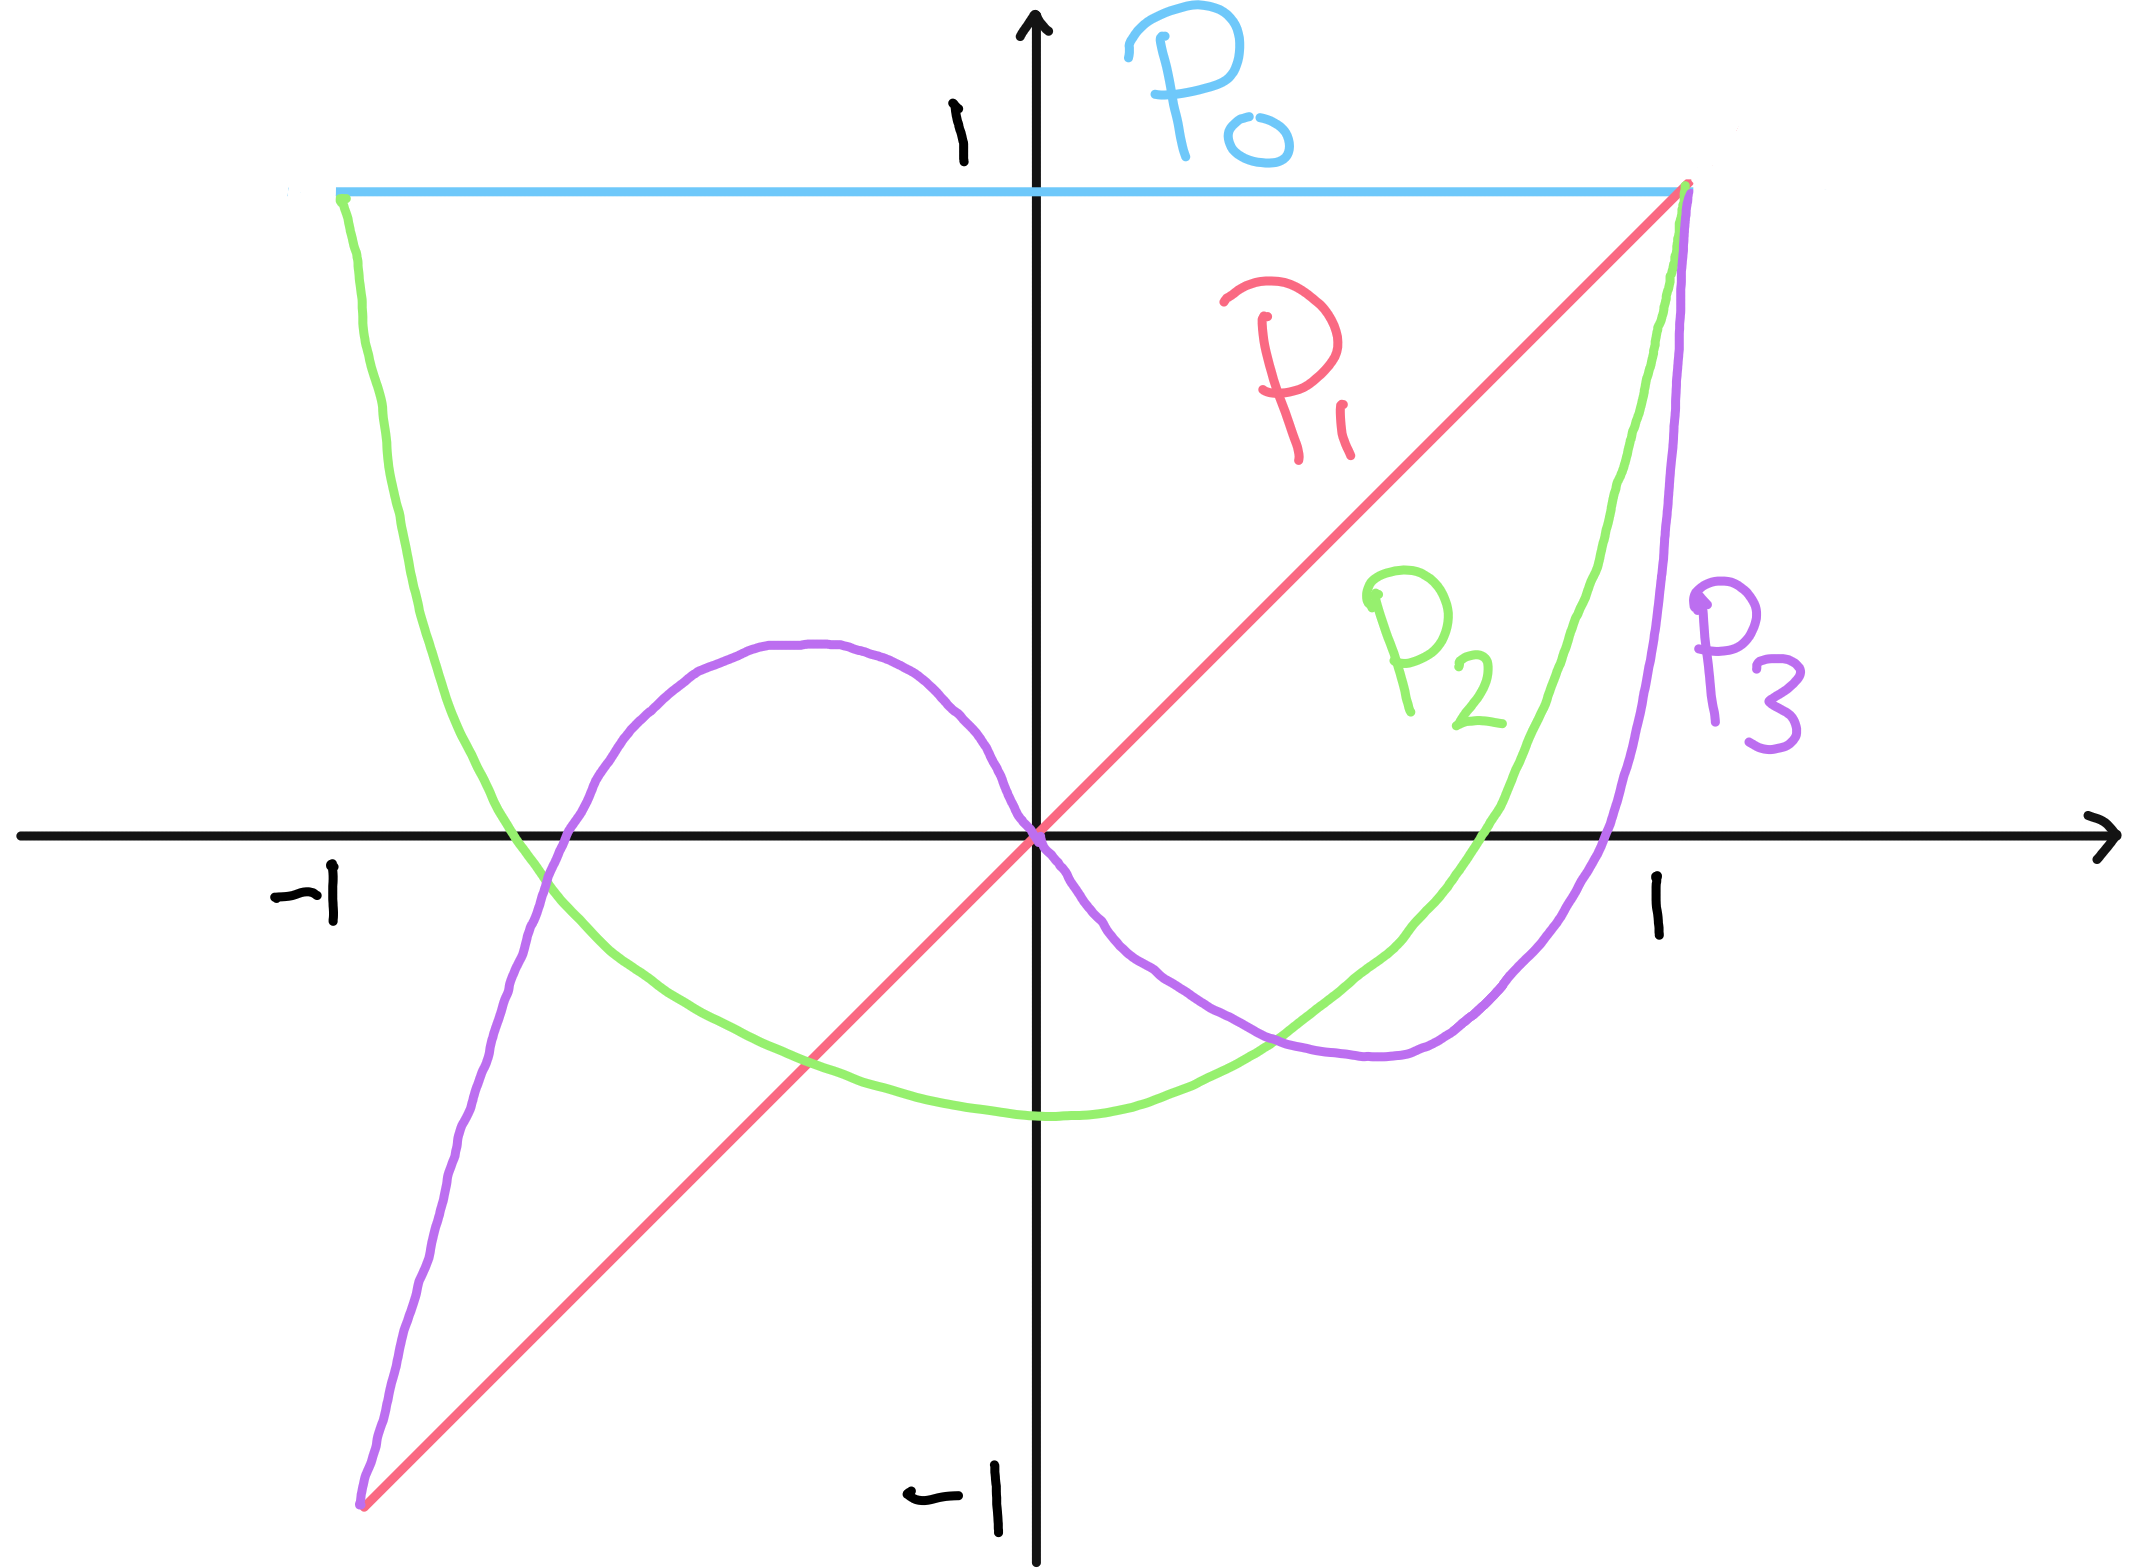
\includegraphics[height=5cm]{02-legendre} 
\end{figure}
\begin{note}
    $P_\ell(x)$ has $\ell$ zeroes.
    $P_\ell$ is odd if $\ell$ is odd, $P_\ell$ is even for even $\ell$.
\end{note} 

\subsection{Properties of Legendre polynomials}
Since Legendre polynomials come from a self-adjoint operator, they must have certain conditions, such as orthogonality.
For $n \neq m$,
\begin{align*}
    \int_{-1}^1 P_n P_m \dd{x} = 0
\end{align*}
They are also normalisable,
\addtocounter{equation}{1}
\begin{align} \label{eq:2.24}
    \int_{-1}^1 P_n^2 \dd{x} = \frac{2}{2n+1}
\end{align}
We can prove this with Rodrigues' formula (Sheet 2, Q5):
\begin{align*}
    P_n(x) = \frac{1}{2^n n!} \qty( \dv{x} )^n (x^2 - 1)^n
\end{align*}
Alternatively we could use a generating function:
\addtocounter{equation}{-2}
\begin{subequations}
    \begin{align} \label{eq:2.23a}
        \sum_{n=0}^\infty P_n(x) t^n &= \frac{1}{\sqrt{1 - 2xt + t^2}} \\
        &= 1 + \frac{1}{2}\qty(2xt - t^2) + \frac{3}{8}\qty(2xt - t^2)^2 + \dots \notag \\
        & = 1 + xt + \frac{1}{2}\qty(3x^2 - 1)t^2 + \dots \notag \\
        &= P_0 + P_1 t + P_2 t^2 + \dots \notag
    \end{align}
\end{subequations}

\begin{exercise}
    Verify $P_3$ and find $P_4$ using binomial expansion.
\end{exercise} 
There are some useful recursion relations\footnote{Derived in Example Sheet}.
\begin{align*}
    \ell(\ell + 1) P_{\ell + 1}(x) = (2 \ell + 1) x P_\ell(x) - \ell P_{\ell - 1}(x)
\end{align*}
Also,
\begin{align*}
    (2\ell + 1)P_\ell(x) = \dv{x} \qty[ P_{\ell + 1}(x) - P_{\ell - 1}(x) ]
\end{align*}

\subsection{Legendre polynomials as eigenfunctions}
Any (well-behaved) function $f(x)$ on $[-1,1]$ can be expressed as
\addtocounter{equation}{1}
\begin{align} \label{eq:2.25}
    f(x) = \sum_{\ell = 0}^\infty a_\ell P_\ell(x)
\end{align}
where
\begin{align} \label{eq:2.26}
    a_\ell = \frac{2\ell + 1}{2} \int_{-1}^1 f(x) P_\ell(x) \dd{x}
\end{align}
with no boundary conditions (e.g.\ periodicity conditions) on $f$.

\begin{exercise}
    Verify $f(x) = \frac{15}{2} x^2 - \frac{3}{2} = P_0(x) + 5 P_2(x)$ using \cref{eq:2.26}
\end{exercise} 

\subsection{Solving inhomogeneous differential equations}
\textit{This can be thought of as the general case of Fourier series discussed previously.}

Consider the problem
\begin{align} \label{eq:2.27}
    \mathcal L y = f(x) \equiv w(x) F(x)
\end{align}
on $x \in [a,b]$ assuming homogeneous boundary conditions.
Given eigenfunctions $y_n(x)$ satisfying $\mathcal L y_n = \lambda_n w y_n$, we wish to expand this solution as (recall \cref{sec:1.6})
\begin{align*}
    y(x) = \sum_n c_n y_n(x)
\end{align*}
and
\begin{align*}
    F(x) = \sum_n a_n y_n(x)
\end{align*}
where $a_n$ are known and $c_n$ are unknown.
Using \cref{eq:2.17}:
\begin{align*}
    a_n = \frac{\int_a^b w F y_n \dd{x}}{\int_a^b w y_n^2 \dd{x}}
\end{align*}
Substituting,
\begin{align*}
    \mathcal L y = \mathcal L \sum_n c_n y_n = w \sum_n c_n \lambda_n y_n = w \sum_n a_n y_n
\end{align*}
By orthogonality,
\begin{align*}
    c_n \lambda_n = a_n \implies c_n = \frac{a_n}{\lambda_n}
\end{align*}
In particular,
\begin{align} \label{eq:2.28}
    y(x) = \sum_{n=1}^\infty \frac{a_n}{\lambda_n}y_n(x)
\end{align} (assuming $\lambda_n \neq 0, \forall \; n$).

We can further generalise; we can permit a driving force, which often induces a linear response term $\widetilde\lambda w y$.
\begin{align} \label{eq:2.29}
    \mathcal L y - \widetilde \lambda w y = f(x)
\end{align}
where $\widetilde \lambda$ is fixed.
The solution \cref{eq:2.28} becomes
\begin{align} \label{eq:2.30}
    y(x) = \sum_{n=1}^\infty \frac{a_n}{\lambda_n - \widetilde \lambda} y_n(x)
\end{align} (again $\widetilde \lambda \neq \lambda_n, \forall \; n$).

\subsection{Integral solutions and Green's function}
Recall \cref{eq:2.28}
\begin{align*}
    y(x) = \sum_{n=1}^\infty \frac{a_n}{\lambda_n} y_n(x) = \sum_n \frac{y_n(x)}{\lambda_n N_n} \int_a^b w(\xi) F(\xi) y_n(\xi) \dd{\xi} \text{ by \cref{eq:2.17}}
\end{align*}
where
\begin{align*}
    N_n = \int w y_n^2 \dd{x}
\end{align*}
This then gives
\begin{align}
    y(x) &= \int_a^b \underbrace{\sum_{n=1}^\infty \frac{y_n(x) y_n(\xi)}{\lambda_n N_n}}_{G(x,\xi)} \underbrace{w(\xi) F(\xi)}_{f(\xi)} \dd{\xi} \notag\\
    &= \int_a^b G(x;\xi) f(\xi) \dd{\xi} \label{eq:2.31}
\end{align}
where
\begin{align*}
    G(x,\xi) = \sum_{n=1}^\infty \frac{y_n(x) y_n(\xi)}{\lambda_n N_n}
\end{align*}
is the eigenfunction expansion of the Green's function.
Note that the Green's function does not depend on $f$, but only on $\mathcal L$ and the boundary conditions.
In this sense, it acts like an inverse operator
\begin{align*}
    \mathcal L\inv \equiv \int \dd{\xi} G(x,\xi)
\end{align*}
analogously to how $Ax = b \implies x = A^{-1} b$ for matrix equations.
    % \part{PDEs on Bounded Domains}
    \part{PDEs on Bounded Domains}

\section{The Wave Equation}

\subsection{Waves on an elastic string}
Consider a small displacement $y(x,t)$ on a stretched string with fixed ends at $x = 0$ and $x = L$, that is, with boundary conditions
\begin{align} \label{eq:3.1}
	y(0,t) = y(L,t) = 0.
\end{align} 
and initial conditions
\begin{align} \label{eq:3.2}
	y(x, 0) = p(x),\ \frac{\partial y}{\partial t}(x,0) = q(x)
\end{align} 
We derive the equation of motion governing the motion of the string by balancing forces on a string segment $(x,x+\delta x)$ and take the limit as $\delta x \to 0$.
\begin{figure}[h] 
	\centering 
	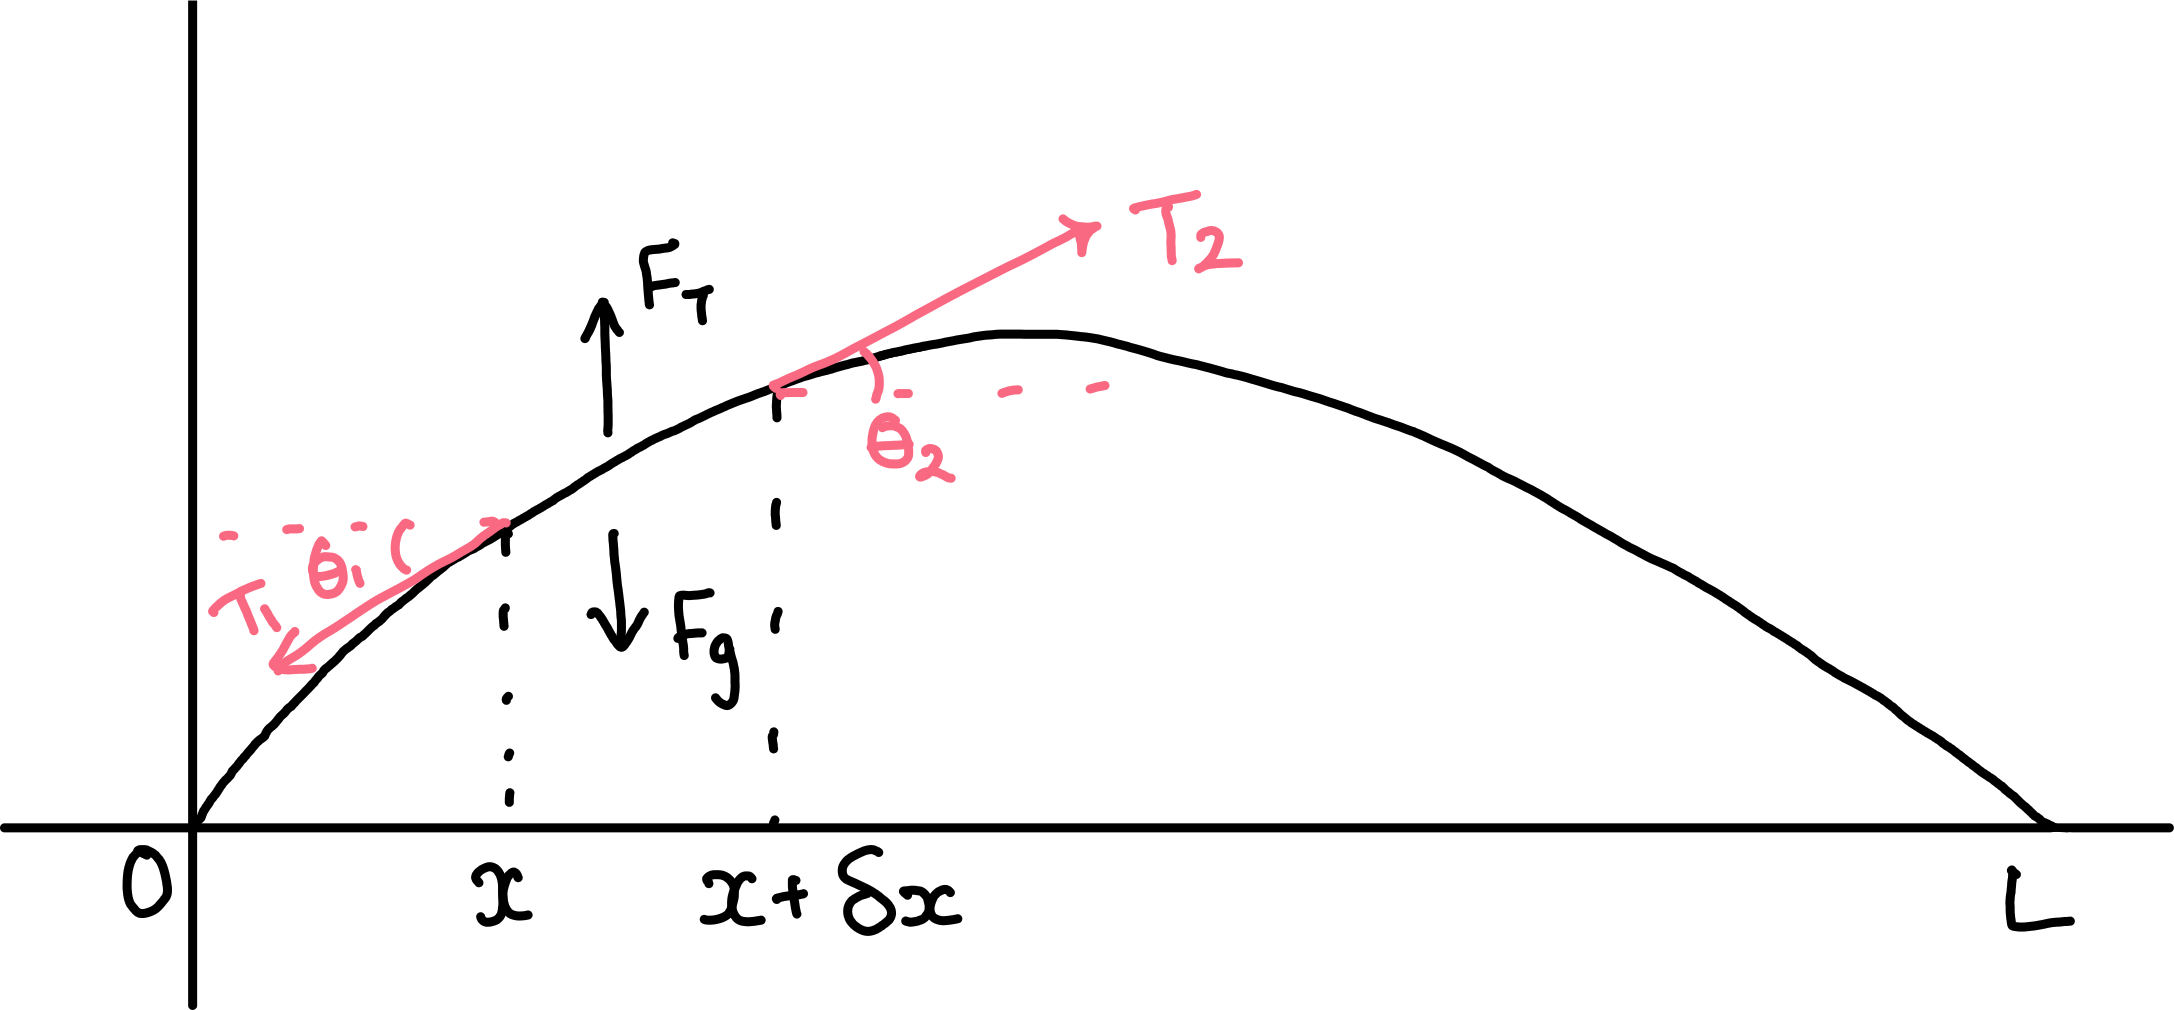
\includegraphics[height=5cm]{03-string} 
\end{figure}

Let $T_1$ be the tension force acting to the left at angle $\theta_1$ from the horizontal.
Analogously, let $T_2$ be the rightwards tension force at angle $\theta_2$.
We assume at any point on the string that $\abs{\pdv{y}{x}} \ll 1$, so the angles of the forces, $\theta_1, \theta_2$ are small.
In the $x$ dimension,
\begin{align*}
	T_1 \cos \theta_1 = T_2 \cos \theta_2 \implies T_1 \approx T_2 = T \text{ by small angle approximation}
\end{align*}
So the tension $T$ is a constant independent of $x$ up to an error of order $O\qty(\abs{\pdv{y}{x}
}^2)$.
In the $y$ dimension, since the $\theta$ are small,
\begin{align*}
	F_T = T_2 \sin \theta_2 - T_1 \sin \theta_1 \approx T \qty(\eval{\pdv{y}{x}}_{x + \delta x} - \eval{\pdv{y}{x}}_x) \approx T \pdv[2]{y}{x} \delta x
\end{align*}
By $F = ma$,
\begin{align*}
	F_T + F_g = (\mu \, \delta x) \pdv[2]{y}{t} = T \pdv[2]{y}{x} \delta x - g \mu \delta x
\end{align*}
where $F_g$ is the gravitational force and $\mu$ is the mass per unit length (linear mass density).
We define the wave speed as
\begin{align*}
	c = \sqrt{\frac{T}{\mu}} \text{ (a constant)}
\end{align*}
and find
\begin{align}
	\pdv[2]{y}{t} = \frac{T}{\mu} \pdv[2]{y}{x} - g = c^2 \pdv[2]{y}{x} - g \label{eq:3.3}
\end{align}
We often assume gravity is negligible to produce the pure wave equation
\begin{align} \label{eq:3.4}
	\frac{1}{c^2} \pdv[2]{y}{t} = \pdv[2]{y}{x}.
\end{align}
The 1D wave equation is then $\ddot{y} = c^2 y''$.

\subsection{Separation of variables}
We wish to solve the wave equation \cref{eq:3.4} subject to  boundary conditions \cref{eq:3.1} and initial conditions \cref{eq:3.2}.
Consider a possible solution of \underline{seperable form} (ansatz):
\begin{align} \label{eq:3.5}
	y(x,t) = X(x) T(t)
\end{align}
Substituting into the wave equation \cref{eq:3.4},
\begin{align*}
	\frac{1}{c^2} \ddot y = y'' \implies \frac{1}{c^2} X \ddot T = X'' T.
\end{align*}
Then
\begin{align*}
	\frac{1}{c^2}\frac{\ddot T}{T} = \frac{X''}{X}
\end{align*}
However, $\frac{\ddot T}{T}$ depends only on $t$ and $\frac{X''}{X}$ depends only on $x$.
Thus, both sides must be equal to some \textit{separation constant} $-\lambda$.
\begin{align*}
	\frac{1}{c^2}\frac{\ddot T}{T} = \frac{X''}{X} = -\lambda
\end{align*}
Hence,
\begin{align}
	X'' + \lambda X &= 0 \label{eq:3.6} \\ 
	\ddot T + \lambda c^2 T &= 0. \label{eq:3.7}
\end{align}

\subsection{Boundary conditions and normal modes}
We will begin by first solving the spatial ODE \cref{eq:3.6}.
One of $\lambda > 0, \lambda < 0, \lambda = 0$ must be true.
The boundary conditions \cref{eq:3.1} restrict the possible $\lambda$.
\begin{enumerate}
	\item First, suppose $\lambda < 0$.
	      Take $\chi^2 = -\lambda$.
	      Then,
	      \begin{align*}
		      X(x) = Ae^{\chi x} + Be^{-\chi x} = \tilde A \cosh (\chi x) + \tilde B \sinh (\chi x).
	      \end{align*}
	      The boundary conditions are $x(0) = x(L) = 0$, so only the trivial solution is possible: $\tilde A = \tilde B = 0$.
	\item Now, suppose $\lambda = 0$.
	      Then
	      \begin{align*}
		      X(x) = Ax + B.
	      \end{align*}
	      Again, the boundary conditions impose $A = B = 0$ giving only the trivial solution.
	\item Finally, the last possibility is $\lambda > 0$.
	      \begin{align*}
		      X(x) = A \cos \qty(\sqrt{\lambda} x) + B \sin \qty(\sqrt{\lambda} x)
	      \end{align*}
	      The boundary conditions give
	      \begin{align*}
		      A = 0;\quad B \sin \qty(\sqrt{\lambda} L) = 0 \implies \sqrt{\lambda} L = n \pi.
	      \end{align*}
		  The following are the eigenfunctions and eigenvalues.
		\begin{align}
			X_n(x) = B_n \sin \frac{n \pi x}{L};\quad \lambda_n = \qty(\frac{n \pi}{L})^2 \ (n > 0) \label{eq:3.8}
		\end{align}
\end{enumerate}

These are also called the \vocab{normal modes} of the system because the spatial shape in $x$ does not change in time, but the amplitude may vary. \\
The fundamental mode is the lowest frequency of vibration, given by
\begin{align*}
	n = 1 \implies \lambda_1 = \frac{\pi^2}{L^2}
\end{align*}
\begin{figure}[h] 
    \centering 
    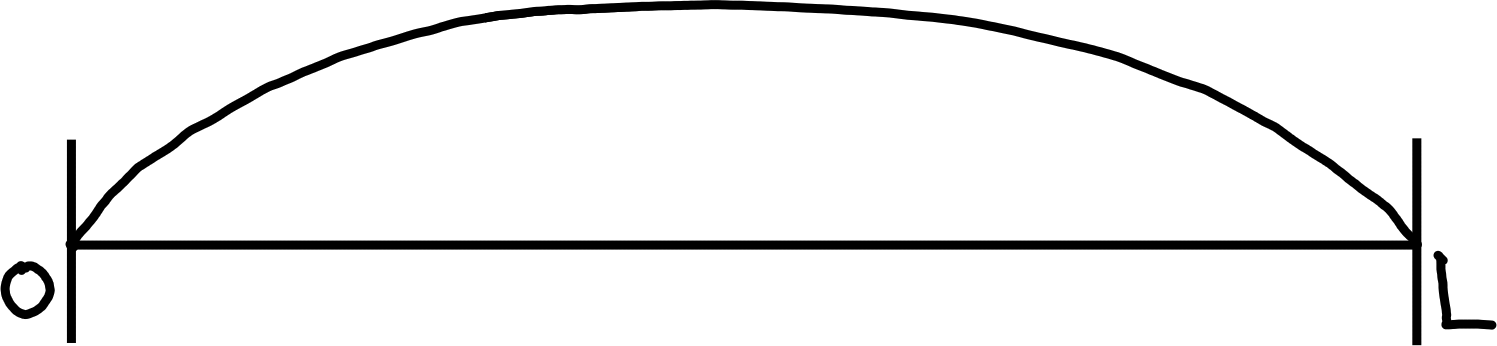
\includegraphics[height=5cm]{03-firstharmonic} 
\end{figure}
The second mode is the first overtone, and is given by
\begin{align*}
	n = 2 \implies \lambda_2 = \frac{4\pi^2}{L^2}
\end{align*}
\begin{figure}[h] 
    \centering 
    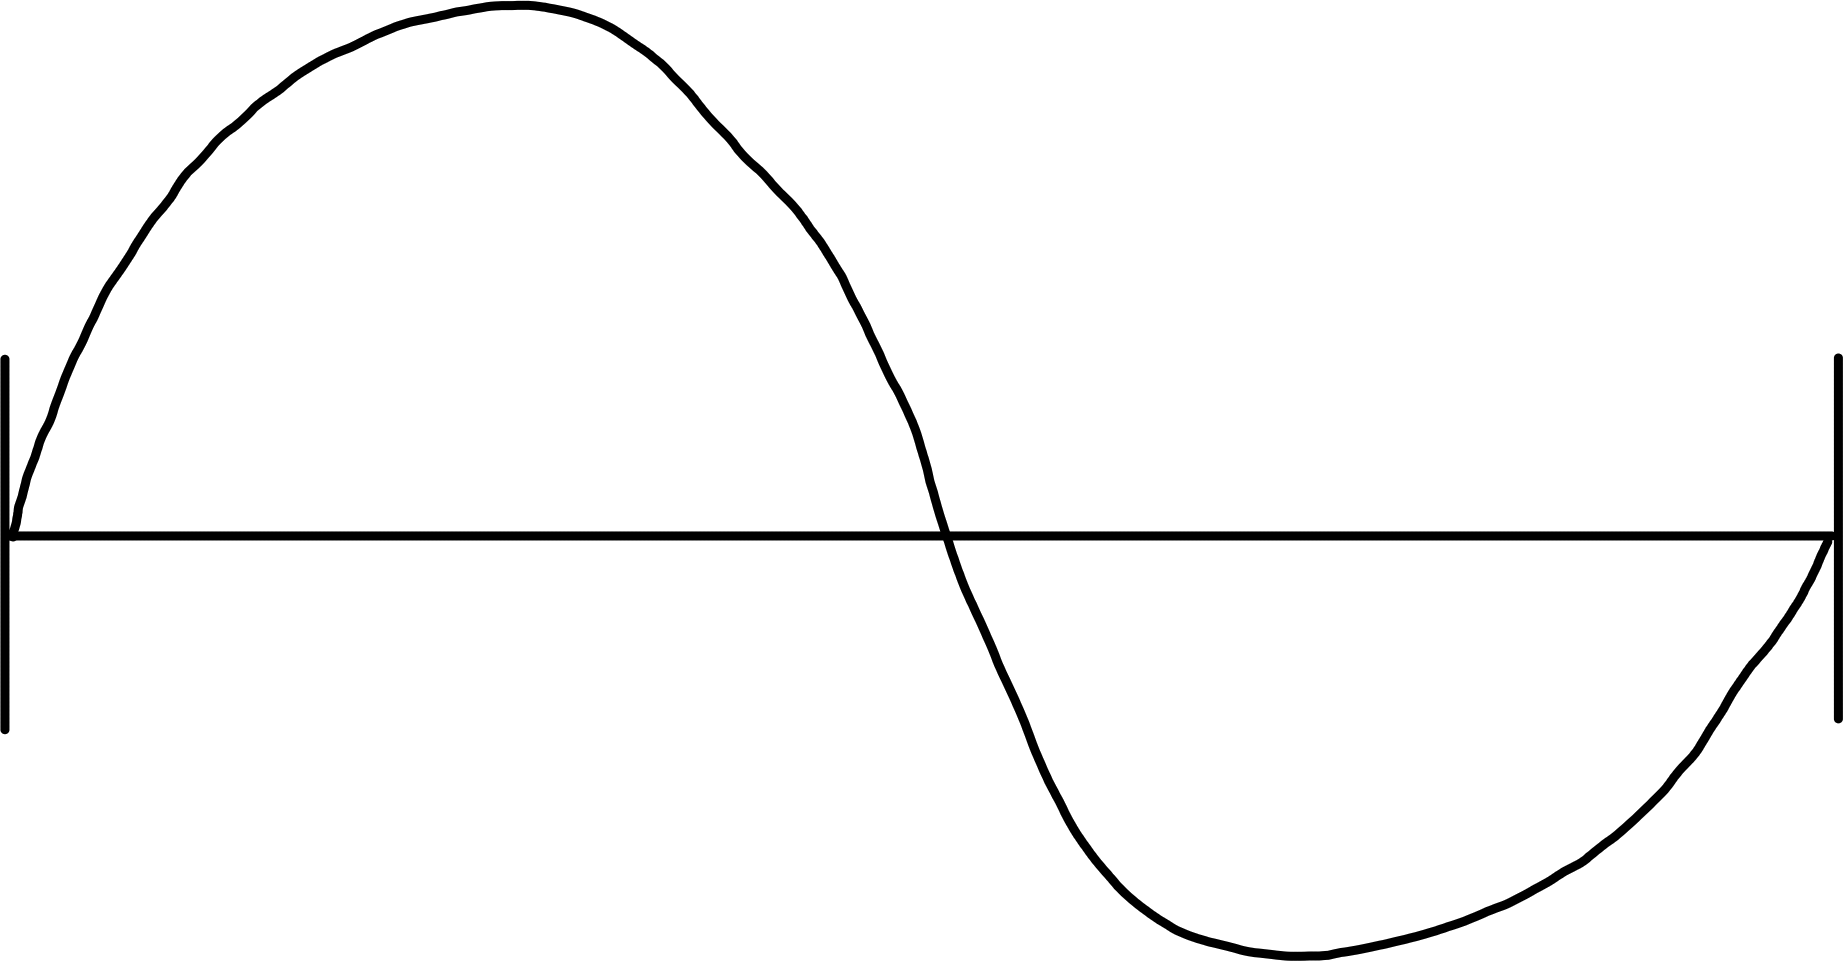
\includegraphics[height=5cm]{03-secondharmonic} 
\end{figure}

\subsection{Initial conditions and temporal solutions}
Substituting $\lambda_n$ into the time ODE \cref{eq:3.7},
\begin{align*}
	\ddot T + \frac{n^2 \pi^2 c^2}{L^2}T = 0.
\end{align*}
Hence,
\begin{align} \label{eq:3.9}
	T_n(t) = C_n \cos \frac{n \pi c t}{L} + D_n \sin \frac{n \pi c t}{L}.
\end{align}

Therefore, a specific solution of the wave equation, \cref{eq:3.4}, satisfying the boundary conditions, \cref{eq:3.1}, is (absorbing the $B_n$ into the $C_n, D_n$):
\begin{align*}
	y_n(x,t) = T_n(t) X_n(x) = \qty(C_n \cos \frac{n \pi c t}{L} + D_n \sin \frac{n \pi c t}{L}) \sin \frac{n \pi x}{L}
\end{align*}

\begin{exercise}
	Verify it's a solution.
\end{exercise} 

Since the wave equation \cref{eq:3.4} is linear (and b.c.s \cref{eq:3.1} are homogenous) we can add the solutions (the $y_n$) together to find \vocab{general string solution}
% To find a particular solution for a given set of initial conditions, we must consider a linear superposition of all possible $y_n$.
\begin{align} \label{eq:3.10}
	y(x,t) = \sum_{n=1}^\infty \qty(C_n \cos \frac{n \pi c t}{L} + D_n \sin \frac{n \pi c t}{L}) \sin \frac{n \pi x}{L}.
\end{align}
By construction, this $y(x,t)$ satisfies the boundary conditions, so now we can impose the initial conditions \cref{eq:3.2}:
\begin{align*}
	y(x,0) = p(x) = \sum_{n=1}^\infty C_n \sin \frac{n \pi x}{L}
\end{align*}
We can find the $C_n$ using standard Fourier series techniques \cref{eq:1.12}, since this is exactly a half-range sine series.
Further,
\begin{align*}
	\pdv{y(x,0)}{t} = q(x) = \sum_{n=1}^\infty \frac{n \pi c}{L} D_n \sin \frac{n \pi x}{L}
\end{align*}
Again we can solve for the $D_n$ in a similar way.
Using \cref{eq:1.12}:
\begin{align}
	\begin{aligned} \label{eq:3.11}
		C_n &= \frac{2}{L} \int_0^L p(x) \sin \frac{n \pi x}{L} \dd{x} \\
		D_n &= \frac{2}{n \pi c} \int_0^L q(x) \sin \frac{n \pi x}{L} \dd{x}
	\end{aligned}
\end{align} 

Hence \cref{eq:3.11} is the solution to \cref{eq:3.4} satisfying \cref{eq:3.1,eq:3.2}.

\begin{example}
	Consider the initial condition of a see-saw wave parametrised by $\xi$, and let $L = 1$.
	This can be visualised as plucking the string at position $\xi$.
	\begin{align*}
		y(x,0) = p(x) = \begin{cases}
			x(1-\xi) & 0 \leq x < \xi \\
			\xi(1-x) & \xi \leq x < 1
		\end{cases}
	\end{align*}
	We also define
	\begin{align*}
		\pdv{y(x,0)}{t} = q(x) = 0
	\end{align*}
	The Fourier series \cref{eq:1.8} for $p$ is given by
	\begin{align*}
		C_n = \frac{2 \sin n \pi \xi}{(n \pi)^2};\quad D_n = 0
	\end{align*}
	Hence the solution to the wave equation is
	\begin{align*}
		y(x,t) = \sum_{n=1}^\infty \frac{2}{(n \pi)^2} \sin n \pi \xi \sin n \pi x \cos n \pi c t
	\end{align*}
	Take $\xi = \frac{1}{2}, C_{2m} = 0, C_{2m - 1} = \frac{2 (-1)^{m + 1}}{((2m-1) \pi)^2}$ (odd only), e.g. Guitar has $\frac{1}{4} \leq \xi \leq \frac{1}{3}$, Violin $\xi \approx \frac{1}{7}$.
\end{example}

\begin{aside}{Solution in characterstic coordinates}
	Recall sine/cosine summation identities (before \cref{eq:1.1}) which means our general solution \cref{eq:3.10} becomes
	\begin{align}
		y(x, t) &= \frac{1}{2} \sum_{n=1}^{\infty} \qty[C_n \sin \frac{n \pi}{L} (x-ct) + D_n \cos \frac{n \pi}{L} (x - ct) + C_n \sin \frac{n \pi}{L} (x + ct) + D_n \cos \frac{n \pi}{L} (x + ct)] \notag \\
		&\equiv f(x - ct) + g(x + ct) \label{eq:3.12}
	\end{align} 
	The standing wave solution \cref{eq:3.10} is made up of a right-moving wave (along characteristic $x - ct = \eta$, $\eta$ a constant) and a left-moving wave ($x + ct = \xi$, $\xi$ a constant) i.e. a general solution with arbitrary $f, g$ (see later).

	\underline{Special case}: $q(x) = 0$ in \cref{eq:3.1} $\implies f = g = \frac{1}{2} D$ at $t = 0$.
	\begin{figure}[h] 
		\centering 
		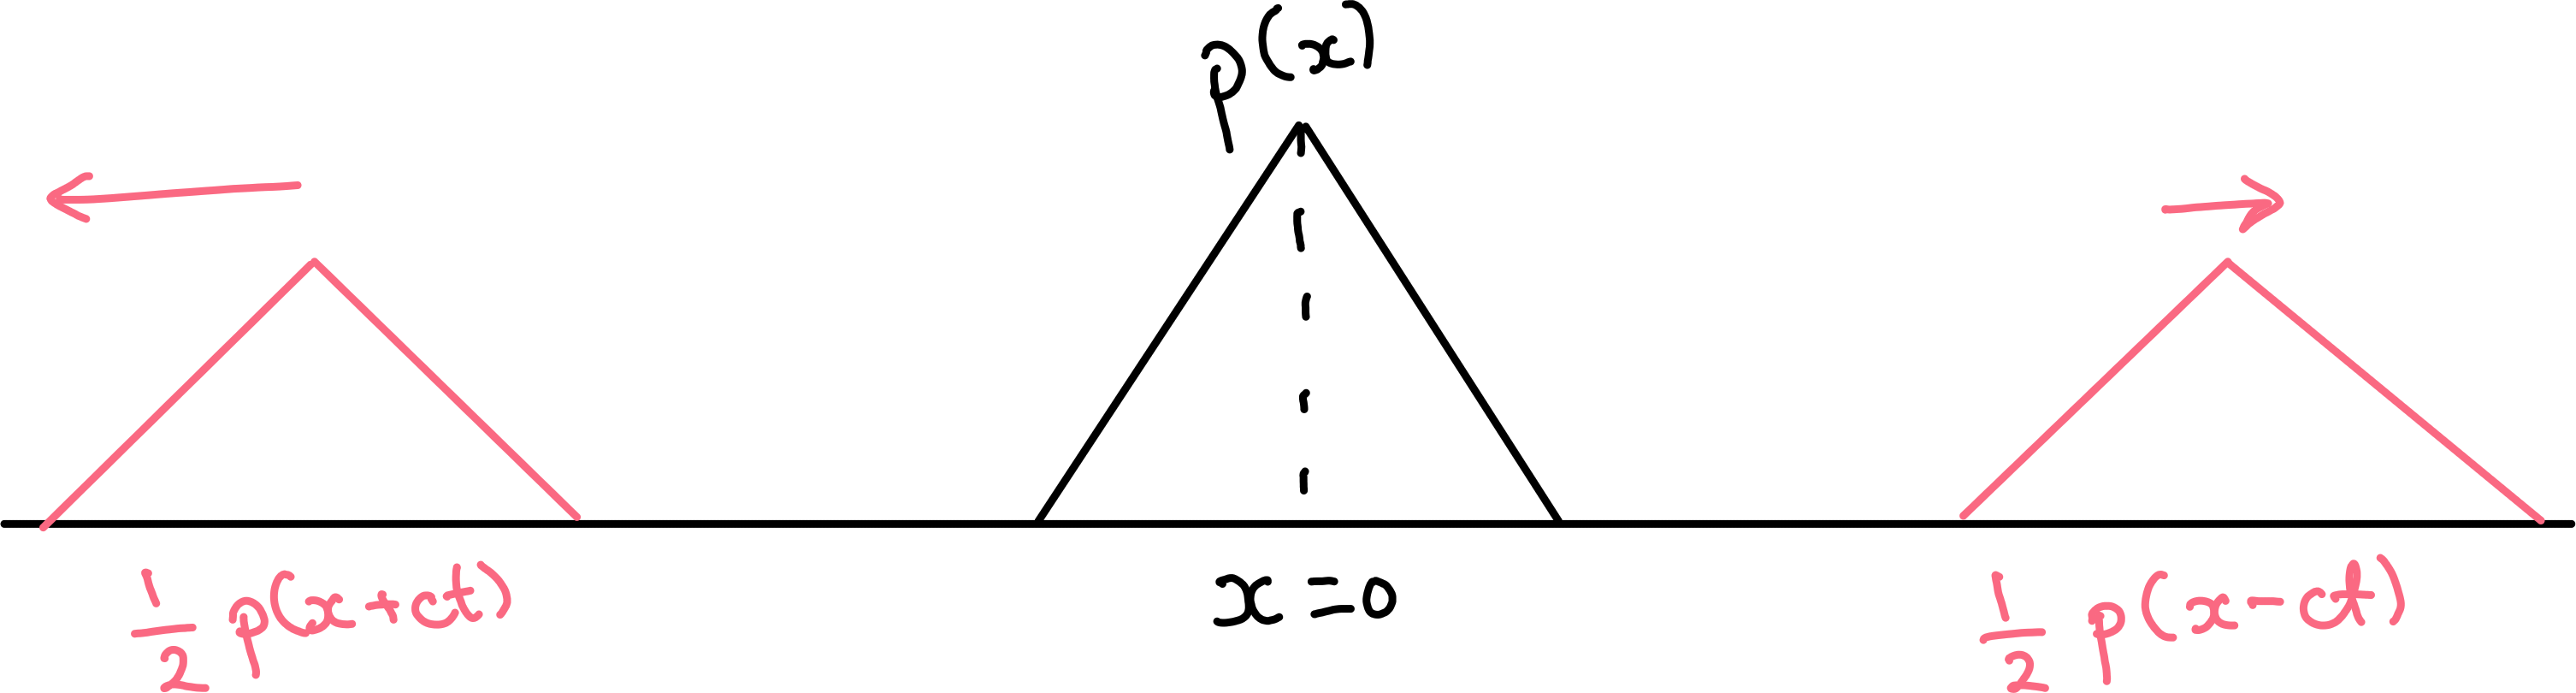
\includegraphics[height=5cm]{03-specialcase} 
	\end{figure}
	
\end{aside} 

\subsection{Separation of variables methodology}
A general strategy for solving higher-dimensional partial differential equations is as follows.
\begin{enumerate}
	\item Obtain a linear PDE system, using boundary and initial conditions.
	\item Separate variables to yield decoupled ODEs.
	\item Impose homogeneous boundary conditions to find eigenvalues and eigenfunctions.
	\item Use these eigenvalues (constants of separation) to find the eigenfunctions in the other variables.
	\item Sum over the products of separable solutions to find the general series solution.
	\item Determine coefficients for this series using the initial conditions.
\end{enumerate}
% \begin{example}
% 	We will solve the wave equation instead in characteristic coordinates.
% 	Recall the sine and cosine summation identities:
% 	\begin{align*}
% 		y(x,t) & = \frac{1}{2} \sum_{n=1}^\infty \Bigg[ \qty(C_n \sin \frac{n \pi}{L}(x-ct) + D_n \cos \frac{n \pi}{L}(x-ct)) \\&
% 		+ \qty(C_n \sin \frac{n \pi}{L}(x+ct) - D_n \cos \frac{n \pi}{L}(x+ct)) \Bigg]                                        \\
% 		       & = f(x-ct) + g(x+ct)
% 	\end{align*}
% 	The standing wave solution can be interpreted as a superposition of a right-moving wave and a left-moving wave.
% 	A special case is $q(x) = 0$, implying $f = g = \frac{1}{2} p$.
% 	Then,
% 	\begin{align*}
% 		y(x,t) = \frac{1}{2}\qty[p(x-ct) + p(x+ct)]
% 	\end{align*}
% \end{example}

\subsection{Energy of oscillations}
A vibrating string has kinetic energy due to its motion.
\begin{align*}
	\text{Kinetic energy} = \frac{1}{2} \mu \int_0^L \qty(\pdv{y}{t})^2 \dd{x}
\end{align*}
It has potential energy  due to stretching by $\Delta x$ given by
\begin{align*}
	\text{Potential energy} = T \Delta x = T \int_c^T \qty(\underbrace{\sqrt{1 + \qty(\pdv{y}{x})^2}}_\text{arc length $s$} -1)\dd{x} \approx \frac{1}{2} T \int_0^L \qty(\pdv{y}{x})^2 \dd{x}
\end{align*}
assuming that the disturbances on the string are small, that is, $\abs{\pdv{y}{x}} \ll 1$.
The total energy on the string, given $c^2 = T/\mu$, is given by
\begin{align} \label{eq:3.13}
	E = \frac{1}{2}\mu \int_0^L \qty[\qty(\pdv{y}{t})^2 + c^2 \qty(\pdv{y}{x})^2] \dd{x}
\end{align}
Substituting the solution \cref{eq:3.10}, using the orthogonality conditions \cref{eq:1.1},
\begin{align}
	E &= \frac{1}{2}\mu \sum_{n=1}^\infty \int_0^L \Bigg[\qty(-\frac{n \pi c}{L} C_n \sin \frac{n \pi c t}{L} + \frac{n \pi c}{L} D_n \cos \frac{n \pi c t}{L})^2 \sin^2 \frac{n \pi x}{L}\notag \\
	&+ c^2 \qty(C_n \cos \frac{n \pi c t}{L} + D_n \sin \frac{n \pi c t}{L})^2 \frac{n^2 \pi^2}{L^2} \cos^2 \frac{n \pi x}{L} \Bigg] \dd{x} \notag \\
	&= \frac{1}{4} \mu \sum_{n=1}^\infty \frac{n^2 \pi^2 c^2}{L} \qty(C_n^2 + D_n^2) \label{eq:3.14}
\end{align}
which is an analogous result to Parseval's theorem.
This is true since \begin{align*}
	\int \cos^2 \frac{n \pi x}{L}\dd{x} = \frac{1}{2}
\end{align*} and $\cos^2 + \sin^2 = 1$.
We can think of this energy as the sum over all the normal modes of the energy in that specific mode.
Note that this quantity is constant over time (no dissipation).

\subsection{Wave reflection and transmission}
Recall the travelling wave solution \cref{eq:3.12}.
The travelling wave has left-moving and right-moving modes.
A \vocab{simple harmonic} travelling wave is
\begin{align*}
	y = \Re\qty[ A e^{i \omega(t-x/c)} ] = A \cos \qty[\omega(t-x/c) + \phi]
\end{align*}
where the phase $\phi$ is equal to $\arg A$, and the wavelength $\lambda$ is $2 \pi c / \omega$.
In further discussion, we assume only the real part is used.

Consider a density discontinuity on the string at $x = 0$ with the following properties.
\begin{align*}
	\mu = \begin{cases}
		\mu_- & \text{for } x < 0 \\
		\mu_+ & \text{for } x > 0
	\end{cases} \implies c = \begin{cases}
		c_- = \sqrt{\frac{T}{\mu_-}} & \text{for } x < 0 \\
		c_+ = \sqrt{\frac{T}{\mu_+}} & \text{for } x > 0 \\
	\end{cases}
\end{align*}
assuming a constant tension $T$.
As a wave from the negative direction approaches the discontinuity, some of the wave will be reflected, given by $B e^{i \omega(t + x/c_-)}$, and some of the wave will be transmitted, given by $D e^{i \omega(t - x/c_+)}$.
\begin{figure}[h] 
    \centering 
    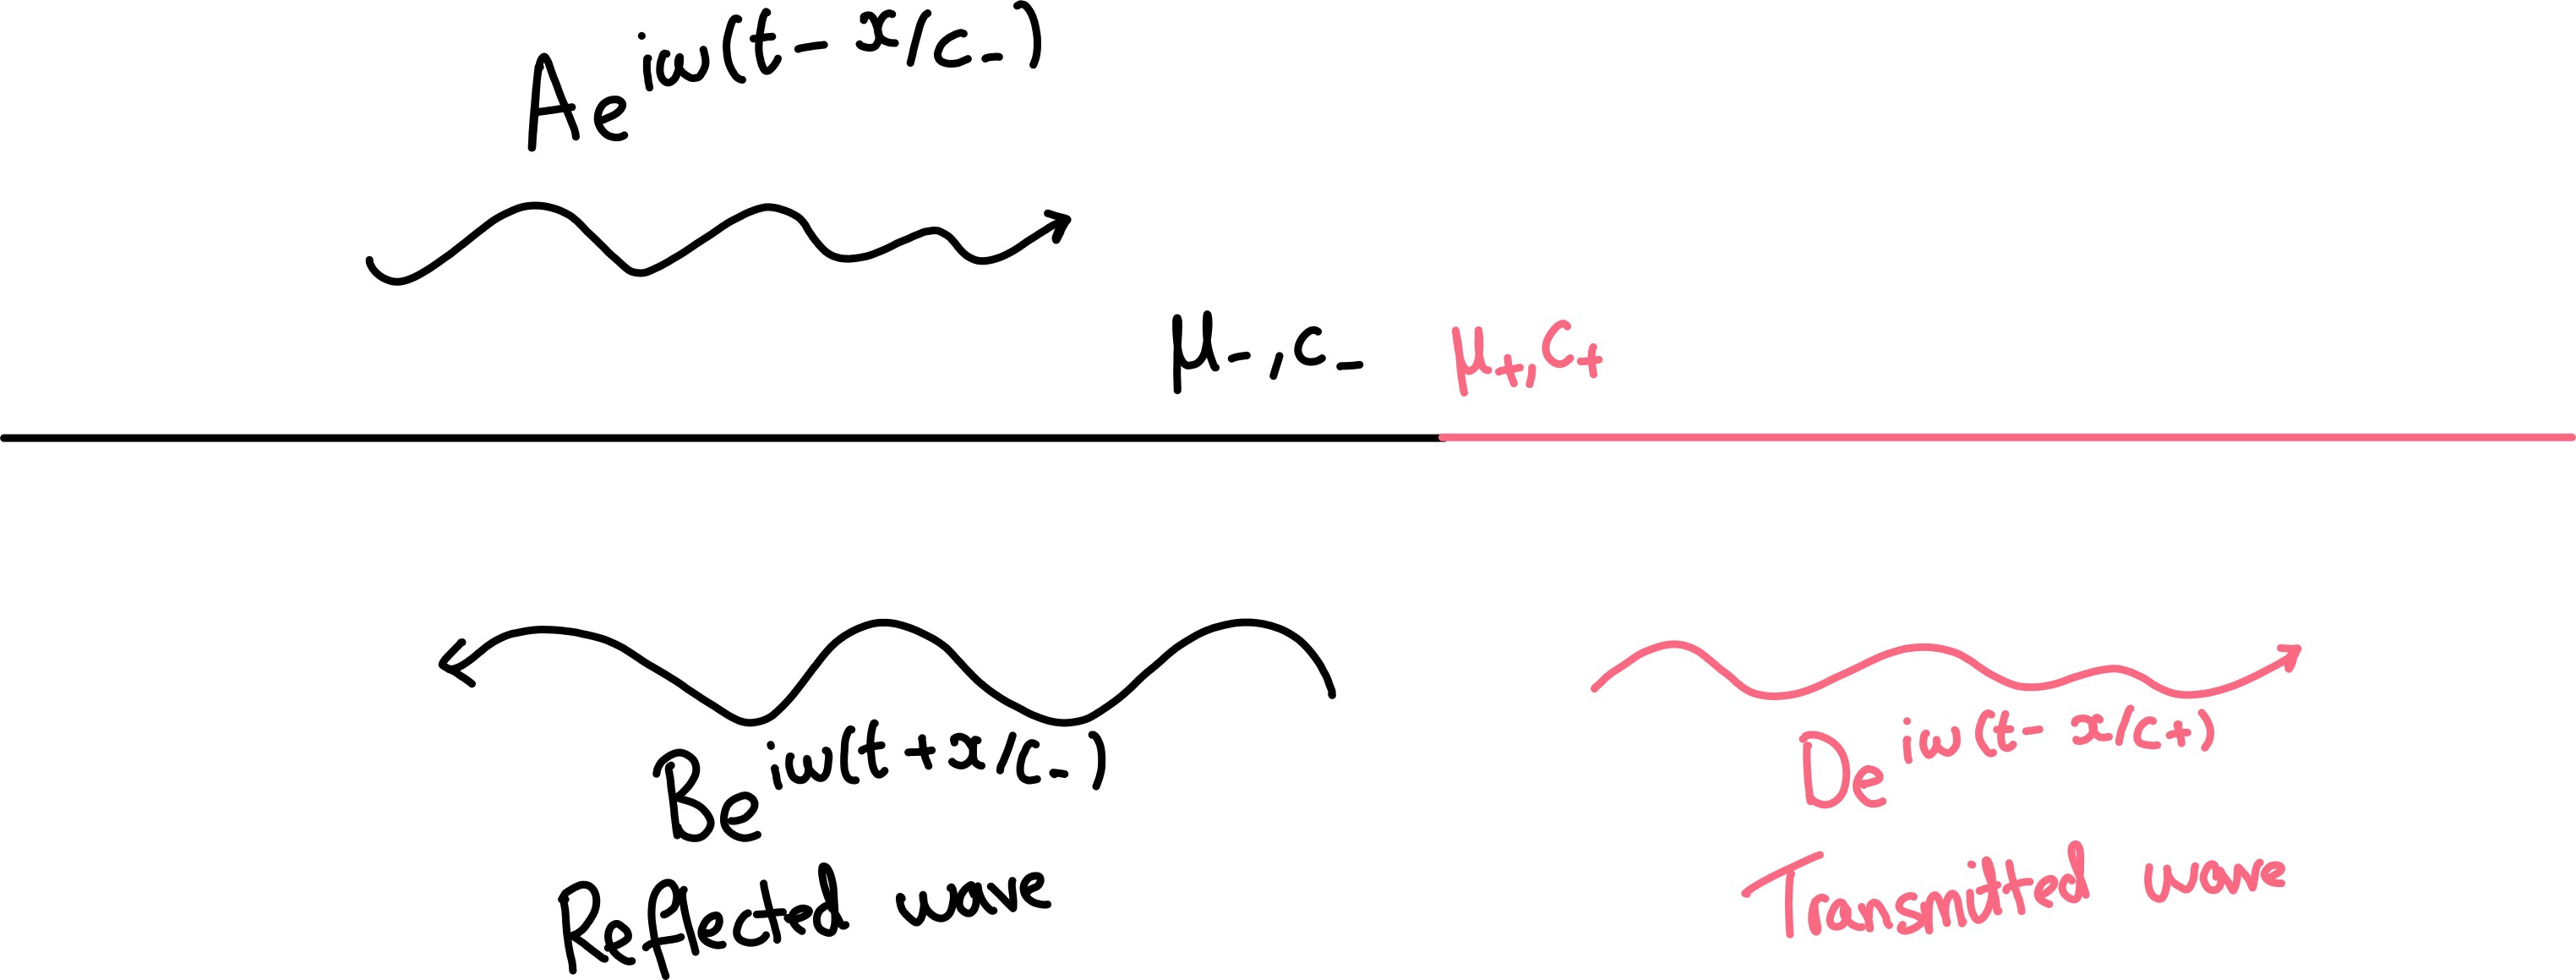
\includegraphics[height=5cm]{03-densitydiscon} 
\end{figure}
The boundary conditions at $x = 0$ are
\begin{enumerate}
	\item $y$ is continuous for all $t$ (the string does not break), so
	\begin{equation}
		A + B = D \tag{$\ast$}
	\end{equation}
	\item The forces balance, $T \eval{\pdv{y}{x}}_{x = 0^-} = T \eval{\pdv{y}{x}}_{x = 0^+}$ which means $\pdv{y}{x}$ must be continuous for all $t$.
	This gives
	\begin{equation}
		\frac{-i\omega A}{c_-} + \frac{i \omega B}{c_-} = \frac{-i \omega D}{c_+} \tag{$\dagger$}
	\end{equation}
\end{enumerate}
We can eliminate $B$ from $(\ast)$ by subtracting $\frac{c_-}{i \omega}(\dagger)$.
\begin{align*}
	2A = D + D \frac{c_-}{c_+} = \frac{D}{c_+}(c_+ + c_-)
\end{align*}
Hence, given $A$, we have the solution for the transmitted amplitude and reflected amplitude to be
\setcounter{equation}{15}
\begin{align} \label{eq:3.16}
	D = \frac{2 c_+}{c_- + c_+} A;\quad B = \frac{c_+ - c_-}{c_- + c_+}
\end{align}
In general $A, B, D$ are complex, hence different phase shifts are possible.

There are a number of limiting cases, for example
\begin{enumerate}
	\item If $c_- = c_+$ we have $D = A$ and $B = 0$ so we have full transmission and no reflection.
	\item (Dirichlet boundary conditions) If $\frac{\mu_+}{\mu_-} \to \infty$, this models a fixed end at $x = 0$.
	      We have $\frac{c_+}{c_-} \to 0$ giving $D = 0$ and $B = -A$.
	      Notice that the reflection has occurred with opposite phase, $\phi = \pi$.
	\item (Neumann boundary conditions) Consider $\frac{\mu_+}{\mu_-} \to 0$, this models a free end.
	      Then $\frac{c_+}{c_-} \to \infty$ giving $D = 2A$, $B = A$.
	      This gives total reflection but with the same phase.
\end{enumerate}

\subsection{Wave equation in 2D plane polar coordinates}
Consider the two-dimensional wave equation for $u(r,\theta,t)$ given by
\begin{align} \label{eq:3.17}
	\frac{1}{c^2} \pdv[2]{u}{t} = \laplacian u
\end{align}
with boundary conditions at $r = 1$ on a unit disc given by
\begin{align} \label{eq:3.18}
	u(1,\theta,t) = 0 \quad \text{(fixed rim)}
\end{align}
and initial conditions for $t = 0$ given by
\begin{align} \label{eq:3.19}
	u(r,\theta,0) = \phi(r,\theta);\quad \pdv{u}{t}(r,\theta,0) = \psi(r,\theta)
\end{align}

\subsubsection{Temporal Seperation}
Suppose that this equation is separable.
First, let us consider temporal separation.
Suppose that
\begin{align} \label{eq:3.20}
	u(r,\theta,t) = T(t) V(r,\theta)
\end{align}
Then substitute into \cref{eq:3.17}
\begin{align}
	\ddot T + \lambda c^2 T &= 0 \label{eq:3.21} \\
	\laplacian V + \lambda V &= 0 \label{eq:3.22}
\end{align}
In plane polar coordinates, we can write the spatial equation \cref{eq:3.22} as
\begin{align*}
	\pdv[2]{V}{r} + \frac{1}{r} \pdv{V}{r} + \frac{1}{r^2}\pdv[2]{V}{\theta} + \lambda V = 0
\end{align*}
\subsubsection{Spatial Seperation}
We will perform another separation, supposing
\begin{align*}
	V(r,\theta) = R(r) \Theta(\theta).
\end{align*}
Substitute into \cref{eq:3.22}
\begin{align}
	\Theta'' + \mu \Theta &= 0 \label{eq:3.23} \\
	r^2 R'' + r R' + \qty(\lambda r^2 - \mu) R &= 0 \label{eq:3.24}
\end{align}
where $\lambda, \mu$ are the separation constants.
\subsubsection{Polar Solution}
The polar solution is constrained by periodicity $\Theta(0) = \Theta(2 \pi)$, since we are working on a disc.
We also consider only $\mu > 0$.
The eigenvalue is then given by $\mu = m^2$, where $m \in \mathbb N \cup \{0\}$.
\begin{align} \label{eq:3.25}
	\Theta_m(\theta) = A_m \cos m \theta + B_m \sin m \theta
\end{align}
Or, in complex exponential form,
\begin{align*}
	\Theta_m(\theta) = C_m e^{im\theta};\quad m \in \mathbb Z
\end{align*}

\subsection{Radial Equations}
We can solve the radial equation \cref{eq:3.24} (in the previous subsection) by converting it first into Sturm-Liouville form \cref{eq:2.7}, which can be accomplished by dividing by $r$ with $\mu = m^2$.
\begin{align} \label{eq:3.26}
	\dv{r} \qty(r R') - \frac{m^2}{r} = -\lambda r R \quad (0 \leq r \leq 1)
\end{align}
where $p(r) = r, q(r) = \frac{m^2}{r}, w(r) = r$, with self-adjoint boundary conditions with $R(1) = 0$.
We will require $R$ is bounded at $R(0)$, and since $p(0) = 0$ there is a regular singular point at $r = 0$.

\subsubsection{Bessel's equation}
This particular equation for $R$ is known as Bessel's equation.
We will first substitute $z \equiv \sqrt{\lambda} r$ in \cref{eq:3.26}, then we find the usual form of Bessel's equation\footnote{May also be written as $(z R')' + (z - m^2 / z) R = 0$},
\begin{align} \label{eq:3.27}
	z^2 \dv[2]{R}{z} + z \dv{R}{z} + (z^2 - m^2)R = 0
\end{align}

\subsubsection{Frobenius Solution}
We can use the method of Frobenius by substituting the following power series:
\begin{align*}
	R = z^p \sum_{n=0}^\infty a_n z^n
\end{align*}
to find
\begin{align*}
	\sum_{n=0}^\infty \qty[ a_n (n+p)(n+p-1) z^{n+p} + (n+p) z^{n+p} + z^{n+p+2} + m^2 z^{n+p} ] = 0
\end{align*}
Equating powers of $z$, we can find the indicial equation
\begin{align*}
	p^2 - m^2 = 0 \implies p = m, -m
\end{align*}
The regular solution, given by $p = m$, has recursion relation
\begin{align*}
	(n+m)^2 a_n + a_{n-2} - m^2 a_n = 0
\end{align*}
which gives
\begin{align*}
	a_n = \frac{-1}{n(n+2m)} a_{n-2}
\end{align*}
Hence, we can find
\begin{align*}
	a_{2n} = a_0 \frac{(-1)^n}{2^{2n} n!
		(n+m)(n+m-1) \dots (m+1)}
\end{align*}
If, by convention, we let
\begin{align*}
	a_0 = \frac{1}{2^m m!}
\end{align*}
we can then write the \textit{Bessel function of the first kind} by
\begin{align} \label{eq:3.28}
	J_m(z) = \qty(\frac{z}{2})^m \sum_{n=0}^\infty \frac{(-1)^n}{n!
		(n+m)!} \qty(\frac{z}{2})^{2n}
\end{align}

\begin{exercise}
	Use $y = \sqrt{z} R$ in Bessel's eqn \cref{eq:3.27} to find $y'' + y (1 + \frac{1}{4z} - \frac{m^2}{z^2})$.
	So, as $z \to \infty$, $y'' = -y$ so we have solns $R = \frac{1}{\sqrt{z}} (A \cos z + B \sin z)$.
\end{exercise}

Also works for $m = \mu$ ($\mu \notin \mathbb{Z}$) if $(n + m)! \to \Gamma(n + m + 1)$.
Second soln with $p = -m$ (integer) is the Neuman function (Bessel function of second kind).
\begin{align*}
	Y_m(z) = \lim_{\mu \to m} \frac{J_\mu \cos(\mu \pi) - J_{-\mu}(z)}{\sin \mu \pi}
\end{align*} 

\begin{exercise}
	Use \cref{eq:3.28} to show that $\frac{d}{dz} (z^m J_m(z)) = z^m J_{m-1}(z)$ and hence
	\begin{align} \label{eq:3.29}
		J'_m(z) + \frac{m}{z} J_m(z) = J_{m-1}(z)
	\end{align}
	Repeat with $z^{-m}$ to find \underline{recursion relations}
	\begin{align} \label{eq:3.30}
		\begin{aligned}
			J_{m-1}(z) + J_{m+1}(z) &= \frac{2m}{z} J_m(z) \\
			J_{m-1}(z) - J_{m+1}(z) &= 2 J'_m(z)
		\end{aligned}
	\end{align} 
\end{exercise} 

\subsection{Asymptotic behaviour of Bessel functions}
If $z$ is small, the leading-order behaviour of $J_m(z)$ is
\begin{align}
	J_0(z) & \approx 1 \notag \\
	J_m(z) & \approx \frac{1}{m!} \qty(\frac{z}{2})^m \notag \\
	Y_0(z) &\to \frac{2}{\pi} \ln(\frac{z}{2}) \notag \\
	Y_m(z) &\to - \frac{(m-1)!}{\pi} (\frac{2}{z})^m \label{eq:3.31}
\end{align}
Now, let us consider large $z$.
In this case, the function becomes oscillatory;
\begin{align}
	J_m(z) &\approx \sqrt{\frac{2}{\pi z}} \cos(z - \frac{m \pi}{2} - \frac{\pi}{4}) \label{eq:3.32} \\
	Y_m(z) &\approx \sqrt{\frac{2}{\pi z}} \sin(z - \frac{m \pi}{2} - \frac{\pi}{4}) \notag
\end{align}

\subsection{Zeroes of Bessel functions $J_m(z)$}
We can see from the asymptotic behaviour that there are infinitely many zeroes of the Bessel functions of the first kind as $z \to \infty$.
We define $j_{mn}$ to be the $n$th zero of $J_m$, for $z > 0$.
Approximately using \cref{eq:3.32},
\begin{align*}
	\cos(z - \frac{m \pi}{2} - \frac{\pi}{4}) = 0 \implies z - \frac{m \pi}{2} - \frac{\pi}{4} = n \pi - \frac{\pi}{2} \quad \text{(modal point)}
\end{align*}
Hence
\begin{align*}
	z \approx n \pi + \frac{m \pi}{2} - \frac{\pi}{4} \equiv \widetilde j_{mn}
\end{align*}

\begin{aside}{Non-examinable}
	Accuracy, 
	\begin{align} \label{eq:3.33}
		\qty| \frac{j_{mn} - \widetilde j_{mn}}{j_{mn}} | < \frac{0.1}{n} \text{ for } n > \frac{m^2}{2}.
	\end{align}
\end{aside} 

For $J_0(z)$ actual values are $J_{01} = 2.405$, $j_{02} = 5.520$, $j_{03} = 8.653$, $j_{0n} = n \pi - \frac{\pi}{4}$ (precision $\approx 1\%/n$).

\begin{figure}[h] 
    \centering 
    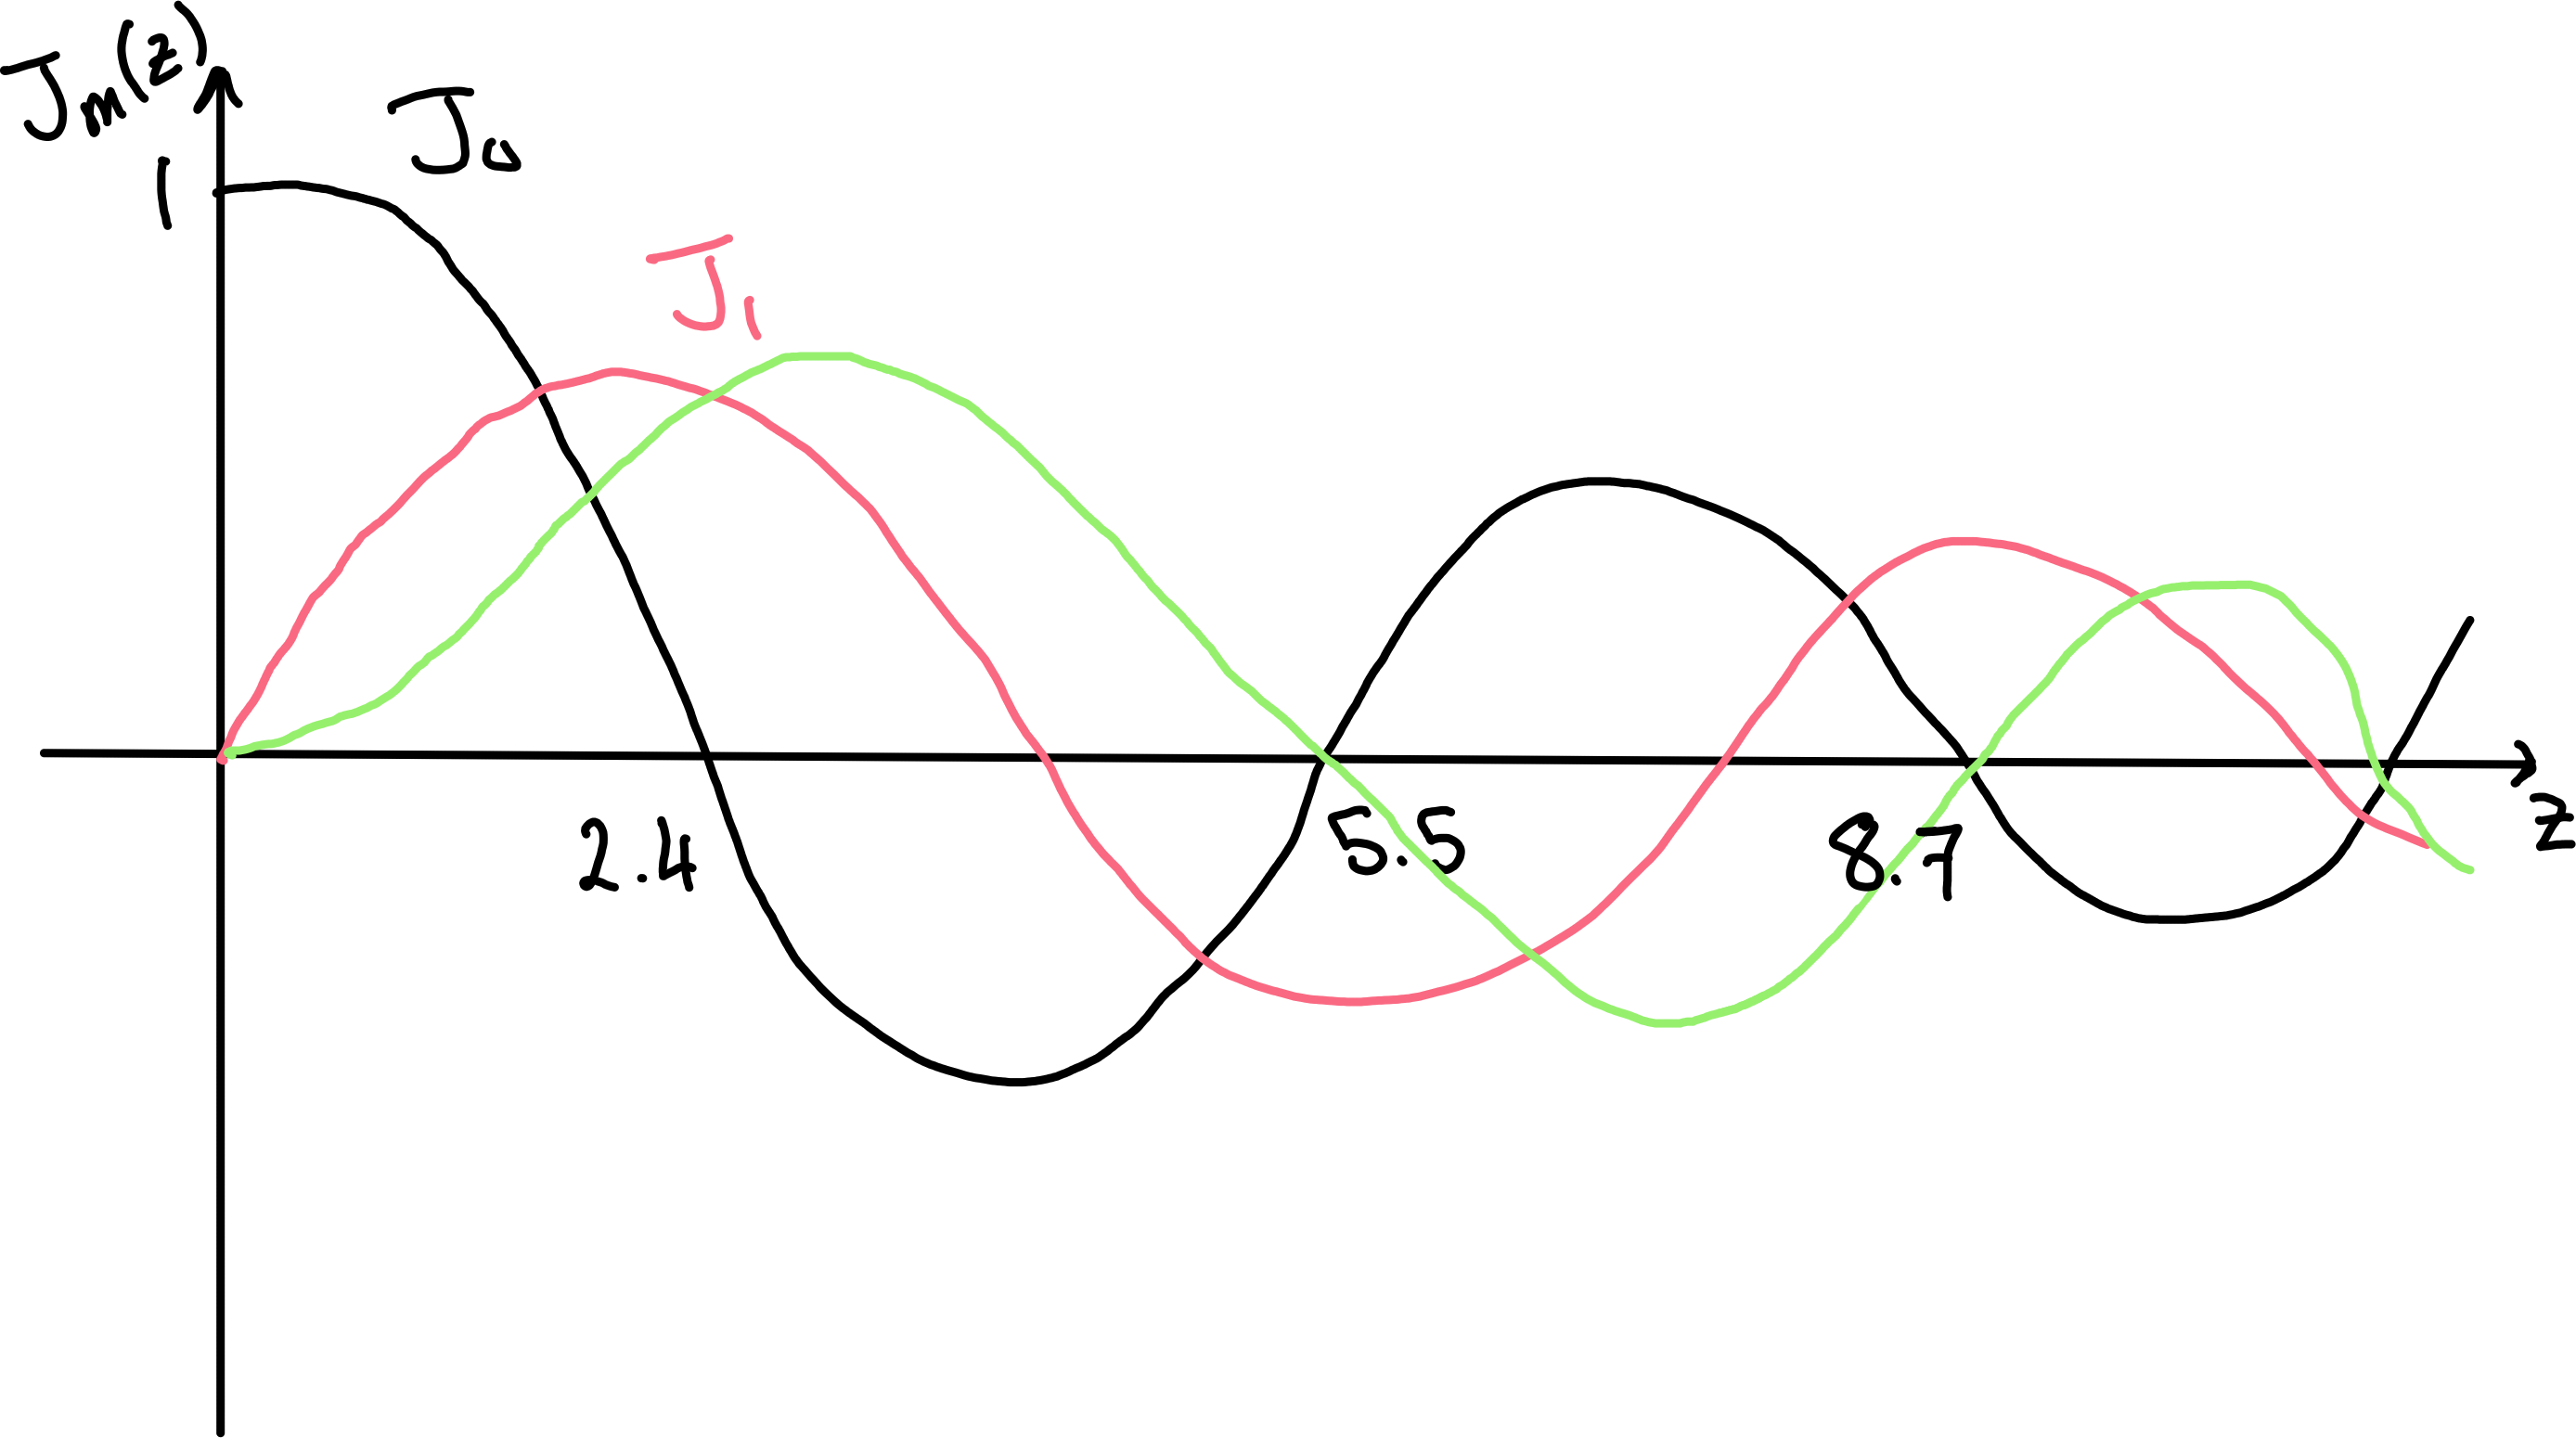
\includegraphics[height=5cm]{03-besselfunctions} 
\end{figure}

\subsection{Solving the vibrating drum}
Recall that the radial solutions to \cref{eq:3.26} become
\begin{align*}
	R_m(z) = R_m(\sqrt{\lambda} x) = A J_m(\sqrt{\lambda} x) + B Y_m(\sqrt{\lambda} x)
\end{align*}
Imposing the boundary condition of boundedness at $r = 0$, we must have $B = 0$ by \cref{eq:3.31}.
Further imposing $r = 1$ and $R = 0$ gives $J_m(\sqrt{\lambda}) = 0$.
These zeroes occur at $j_{mn} \approx n \pi + \frac{m \pi}{2} - \frac{\pi}{4}$.
Hence, the eigenvalues must be 
\begin{align} \label{eq:3.34}
	\lambda = j^2_{mn}.
\end{align}
Therefore, the spatial solution with the polar mode \cref{eq:3.26} is
\begin{align}
	V_{mn}(r, \theta) &= \Theta_m(\theta) R_{mn}(\sqrt{\lambda_{mn}} r) \notag \\
	&= (A_{mn} \cos m \theta + B_{mn} \sin m \theta) J_m (j_{mn} r) \label{eq:3.35}
\end{align}

The temporal solution \cref{eq:3.21} is
\begin{align*}
	\ddot T = -\lambda c^2 T \implies T_{mn}(t) = \cos(j_{mn} ct), \sin(j_{mn} ct)
\end{align*}

Combining everything together, the full solution to \cref{eq:3.17} is
\begin{align}
	\begin{aligned} \label{eq:3.36}
		u(r,\theta,t) & = \sum_{n=1}^\infty J_0(j_{0n} r) \qty( A_{0n}\cos j_{0n}ct + C_{0n}\sin j_{0n}ct ) \\
		&+ \sum_{m=1}^\infty \sum_{n=1}^\infty J_m (j_{mn}r) \qty( A_{mn} \cos m \theta + B_{mn} \sin m\theta ) \cos j_{mn} ct \\
		&+ \sum_{m=1}^\infty \sum_{n=1}^\infty J_m (j_{mn}r) \qty( C_{mn} \cos m \theta + D_{mn} \sin m\theta ) \sin j_{mn} ct
	\end{aligned}
\end{align} 

Now, we impose the \underline{initial conditions} \cref{eq:3.19} at $t = 0$
\begin{align} \label{eq:3.37}
	u(r,\theta,0) = \phi(r,\theta) = \sum_{m=0}^\infty \sum_{n=1}^\infty J_m (j_{mn}r) \qty( A_{mn} \cos m \theta + B_{mn} \sin m\theta )
\end{align}
and
\begin{align*}
	\pdv{u}{t}\qty(r,\theta,0) = \psi(r,\theta) = \sum_{m=0}^\infty \sum_{n=1}^\infty j_{mn} c J_m (j_{mn}r) \qty( C_{mn} \cos m \theta + D_{mn} \sin m\theta )
\end{align*}
We need to find the coefficients by multiplying by $J_m, \cos, \sin$ and using the orthogonality relations (\cref{eq:1.1,eq:1.2,eq:1.3} and Sheet 1, Q8), which are
\begin{align}
	\int_0^1 J_m(j_{mn} r) J_m(j_{mk} r) r \dd{r} &= \frac{1}{2}\qty[J_m'(j_{mn})]^2 \delta_{nk} \label{eq:3.38} \\
	&= \frac{1}{2}\qty[J_{m+1}(j_{mn})]^2 \delta_{nk} \label{eq:3.39}
\end{align}
by using a recursion relation of the Bessel functions.
We can then integrate to obtain the coefficients $A_{mn}$.
\begin{align*}
	\int_0^{2\pi} \dd{\theta} \cos p\theta \int_0^1 r \dd{r} J_p(j_{pq} r) \phi(r,\theta) = \frac{\pi}{2}\qty[J_{p+1}(j_{pq})]^2 A_{pq}
\end{align*}
where the $\frac{\pi}{2}$ coefficient is $2\pi$ for $p = 0$.
\begin{exercise}
	Find the analogous results for the $B_{mn}, C_{mn}, D_{mn}$.
\end{exercise} 
 
\begin{example}
	Consider an initial radial profile $u(r,\theta,0) = \phi(r) = 1 - r^2$.
	Then, $m = 0, B_{mn} = 0$ for all $m$ and $A_{mn} = 0$ for all $m \neq n$.
	Then
	\begin{align*}
		\pdv{u}{t}\qty(r,0,0) = 0
	\end{align*}
	hence $C_{mn}, D_{mn} = 0$.
	We just now need to find
	\begin{align*}
		A_{0n} = \frac{2}{J_1(j_{0n})^2} \int_0^1 J_0(j_{0n}r)(1-r)^2 r\dd{r} = \frac{2}{J_1(j_{0n})^2} \frac{J_2(j_{0n})}{j_{0n}^2} \approx \frac{J_2(j_{0n})}{n} \text{ as } n \to \infty
	\end{align*}
	Proving this is left as an exercise using \cref{eq:3.29,eq:3.30}.
	Then the approximate solution is
	\begin{align*}
		u(r,\theta,t) = \sum_{n=1}^\infty A_{0n} J_0(j_{0n}r)\cos j_{0n} ct
	\end{align*}
	The fundamental frequency is $\omega_d = j_{01} c \frac{2}{d} \approx 4.8\frac{c}{d}$ where $d$ is the diameter of the drum.
	Comparing this to a string with length $d$, this has a fundamental frequency of $\omega_s = \frac{\pi c}{d} \approx 0.77 \omega_d$.
\end{example}
    \section{Diffusion equation}
\subsection{Diffusion equation derivation with Fourier's law}
Fourier's law for heat flow is
\begin{align} \label{eq:4.1}
	q = -k \grad{\theta}
\end{align}
where $q$ is the heat flux, $k$ the thermal conductivity and $\theta$ is the temperature.
In a volume $V$, the overall heat energy $Q$ is given by
\begin{align} \label{eq:4.2}
	Q = \int_V c_V \rho \theta \dd{V}
\end{align}
where $c_V$ is the specific heat of the material, $\rho$ is the mass density.
The rate of change due to heat flow is
\begin{align*}
	\dv{Q}{t} = \int_V c_V \rho \pdv{\theta}{t} \dd{V} \tag{$\ast$}
\end{align*}
We will integrate \cref{eq:4.1} over the surface $S = \partial V$, giving
\begin{align*}
	-\dv{Q}{t} = \int_S q \cdot \hat n \dd{S}
\end{align*}
The negative sign is due to the normals facing outwards.
This is exactly
\begin{align*}
	-\dv{Q}{t} = \int_S (-k \grad{\theta}) \cdot \hat n \dd{S} = \int_V -k \laplacian{\theta} \dd{V} \tag{$\dagger$}
\end{align*}
Equating these two forms (($\ast$) and ($\dagger$)) for $\dv{Q}{t}$, we find
\begin{align*}
	\int_V (c_V \rho \pdv{\theta}{t} - k \laplacian{\theta}) \dd{V} = 0
\end{align*}
Since $V$ was arbitrary, the integrand must be zero.
So we have
\begin{align*}
	\pdv{\theta}{t} - \frac{k}{c_V \rho} \laplacian{\theta} = 0
\end{align*}
Let $D = \frac{k}{c_V \rho}$ be the diffusion constant.
Then we have the diffusion equation
\begin{align} \label{eq:4.3}
	\pdv{\theta}{t} - D \laplacian{\theta} = 0
\end{align}

\subsection{Diffusion equation derivation with statistical dynamics}
We can derive this equation in another way, using statistical dynamics.
Gas particles diffuse by scattering every fixed time step $\Delta t$ with probability density function $p(\xi)$ of moving by a displacement $\xi$.
On average, we have
\begin{align*}
	\mathbb{E}[\xi] = \int p(\xi) \xi \dd{\xi} = 0
\end{align*}
since there is no bias the direction in which any given particle is travelling.
Suppose that the probability density function after $N\Delta t$ time is described by $P_{N \Delta t}(x)$.
Then, for the next time step,
\begin{align*}
	P_{(N+1)\Delta t}(x) = \int_{-\infty}^\infty p(\xi) P_{N \Delta t}(x - \xi) \dd{\xi}
\end{align*}
Using the Taylor expansion,
\begin{align*}
	P_{(N+1)\Delta t}(x) & \approx \int_{-\infty}^\infty p(\xi) \qty[P_{N \Delta t}(x) + P_{N \Delta t}'(x)(-\xi) + P_{N \Delta t}''(x)\frac{\xi^2}{2} + \cdots] \dd{\xi} \\
	& \approx P_{N \Delta t}(x) - P_{N \Delta t}'(x) \mathbb{E}[\xi] + P_{N \Delta t}''(x) \frac{\mathbb{E}[\xi^2]}{2} + \cdots \\
	& \approx P_{N \Delta t}(x) + P_{N \Delta t}''(x) \frac{\mathbb{E}[\xi^2]}{2} + \cdots
\end{align*}
since $\int p(\xi) \dd{\xi} = 1$.
Identifying $P_{N \Delta t}(x) = P(x, N\Delta t)$, we can write
\begin{align*}
	P(x, (N+1)\Delta t) - P(x, N \Delta t) = \pdv[2]{x} P(x, N\Delta t) \frac{\mathbb{E}[\xi^2]}{2}
\end{align*}
Assuming that the variance $\mathbb{E}[\xi^2]$\footnote{$\Var X = \mathbb{E}[X^2] - \mathbb{E}[X]^2$ and $\mathbb{E}[X] = 0$.} is equal to $2D \Delta t$, then for small $\Delta t$, we find
\begin{align} \label{eq:4.4}
	\pdv{P}{t} = D \pdv[2]{P}{x}
\end{align}
which is exactly the diffusion equation.

\subsection{Similarity solutions}
The characteristic relation between the variance and time suggests that we seek solutions with a dimensionless parameter.
If we can find a change of variables of the form $\theta(\eta) = \theta(x,t)$, then it will likely be easier to solve.
Consider
\begin{align} \label{eq:4.5}
	\eta \equiv \frac{x}{2\sqrt{Dt}}
\end{align}
Then changing variables in \cref{eq:4.3},
\begin{align*}
	\pdv{\theta}{t} = \pdv{\eta}{t} \pdv{\theta}{\eta} = \frac{-1}{2} \frac{x}{\sqrt{D} t^{3/2}} \theta' = \frac{-1}{2} \frac{\eta}{t} \theta'
\end{align*}
and
\begin{align*}
	D \pdv[2]{\theta}{x} = D \pdv{x} \qty(\pdv{\eta}{x} \pdv{\theta}{\eta}) = D \pdv{x} \qty(\frac{1}{2\sqrt{Dt}} \theta') = \frac{D}{4Dt} \theta'' = \frac{1}{4t} \theta''
\end{align*}
Equating,
\begin{align} \label{eq:4.6}
	\theta'' = -2 \eta \theta'
\end{align}
Let $\psi = \theta'$.
Then
\begin{align*}
	\frac{\psi'}{\psi} = -2\eta \implies \ln \psi = -\eta^2 + \text{constant}
\end{align*}
Then, choosing a constant of $c\frac{2}{\sqrt{\pi}}$,
\begin{align} \label{eq:4.7}
	\psi = c\frac{2}{\sqrt{\pi}} e^{-\eta^2} \implies \theta(\eta) = c\frac{2}{\sqrt{\pi}} \int_0^\eta e^{-u^2} \dd{u} = c \erf(\eta) = c \erf \qty(\frac{x}{2\sqrt{Dt}})
\end{align}
where
\begin{align*}
	\erf(z) = \frac{2}{\sqrt{\pi}} \int_0^z e^{-u^2} \dd{u}
\end{align*}
This describes discontinuous initial conditions that spread over time.

\begingroup
\tikzset{every picture/.style={scale=1}}
% Recommended preamble:
% \usetikzlibrary{arrows.meta}
% \usetikzlibrary{backgrounds}
% \usepgfplotslibrary{patchplots}
% \usepgfplotslibrary{fillbetween}
% \pgfplotsset{%
%     layers/standard/.define layer set={%
%         background,axis background,axis grid,axis ticks,axis lines,axis tick labels,pre main,main,axis descriptions,axis foreground%
%     }{
%         grid style={/pgfplots/on layer=axis grid},%
%         tick style={/pgfplots/on layer=axis ticks},%
%         axis line style={/pgfplots/on layer=axis lines},%
%         label style={/pgfplots/on layer=axis descriptions},%
%         legend style={/pgfplots/on layer=axis descriptions},%
%         title style={/pgfplots/on layer=axis descriptions},%
%         colorbar style={/pgfplots/on layer=axis descriptions},%
%         ticklabel style={/pgfplots/on layer=axis tick labels},%
%         axis background@ style={/pgfplots/on layer=axis background},%
%         3d box foreground style={/pgfplots/on layer=axis foreground},%
%     },
% }

\begin{tikzpicture}[/tikz/background rectangle/.style={fill={rgb,1:red,1.0;green,1.0;blue,1.0}, draw opacity={1.0}}, show background rectangle]
\begin{axis}[point meta max={nan}, point meta min={nan}, legend cell align={left}, legend columns={1}, title={$D=1$}, title style={at={{(0.5,1)}}, anchor={south}, font={{\fontsize{14 pt}{18.2 pt}\selectfont}}, color={rgb,1:red,0.0;green,0.0;blue,0.0}, draw opacity={1.0}, rotate={0.0}, align={center}}, legend style={color={rgb,1:red,0.0;green,0.0;blue,0.0}, draw opacity={1.0}, line width={1}, solid, fill={rgb,1:red,1.0;green,1.0;blue,1.0}, fill opacity={1.0}, text opacity={1.0}, font={{\fontsize{8 pt}{10.4 pt}\selectfont}}, text={rgb,1:red,0.0;green,0.0;blue,0.0}, cells={anchor={center}}, at={(1.02, 1)}, anchor={north west}}, axis background/.style={fill={rgb,1:red,1.0;green,1.0;blue,1.0}, opacity={1.0}}, anchor={north west}, xshift={1.0mm}, yshift={-1.0mm}, width={145.4mm}, height={99.6mm}, scaled x ticks={false}, xlabel={$x$}, x tick style={color={rgb,1:red,0.0;green,0.0;blue,0.0}, opacity={1.0}}, x tick label style={color={rgb,1:red,0.0;green,0.0;blue,0.0}, opacity={1.0}, rotate={0}}, xlabel style={at={(ticklabel cs:0.5)}, anchor=near ticklabel, at={{(ticklabel cs:0.5)}}, anchor={near ticklabel}, font={{\fontsize{11 pt}{14.3 pt}\selectfont}}, color={rgb,1:red,0.0;green,0.0;blue,0.0}, draw opacity={1.0}, rotate={0.0}}, xmajorgrids={true}, xmin={-3.18}, xmax={3.18}, xticklabels={{$-3$,$-2$,$-1$,$0$,$1$,$2$,$3$}}, xtick={{-3.0,-2.0,-1.0,0.0,1.0,2.0,3.0}}, xtick align={inside}, xticklabel style={font={{\fontsize{8 pt}{10.4 pt}\selectfont}}, color={rgb,1:red,0.0;green,0.0;blue,0.0}, draw opacity={1.0}, rotate={0.0}}, x grid style={color={rgb,1:red,0.0;green,0.0;blue,0.0}, draw opacity={0.1}, line width={0.5}, solid}, axis x line*={left}, x axis line style={color={rgb,1:red,0.0;green,0.0;blue,0.0}, draw opacity={1.0}, line width={1}, solid}, scaled y ticks={false}, ylabel={$\theta$}, y tick style={color={rgb,1:red,0.0;green,0.0;blue,0.0}, opacity={1.0}}, y tick label style={color={rgb,1:red,0.0;green,0.0;blue,0.0}, opacity={1.0}, rotate={0}}, ylabel style={at={(ticklabel cs:0.5)}, anchor=near ticklabel, at={{(ticklabel cs:0.5)}}, anchor={near ticklabel}, font={{\fontsize{11 pt}{14.3 pt}\selectfont}}, color={rgb,1:red,0.0;green,0.0;blue,0.0}, draw opacity={1.0}, rotate={0.0}}, ymajorgrids={true}, ymin={-1.06}, ymax={1.06}, yticklabels={{$-1.0$,$-0.5$,$0.0$,$0.5$,$1.0$}}, ytick={{-1.0,-0.5,0.0,0.5,1.0}}, ytick align={inside}, yticklabel style={font={{\fontsize{8 pt}{10.4 pt}\selectfont}}, color={rgb,1:red,0.0;green,0.0;blue,0.0}, draw opacity={1.0}, rotate={0.0}}, y grid style={color={rgb,1:red,0.0;green,0.0;blue,0.0}, draw opacity={0.1}, line width={0.5}, solid}, axis y line*={left}, y axis line style={color={rgb,1:red,0.0;green,0.0;blue,0.0}, draw opacity={1.0}, line width={1}, solid}, colorbar={false}]
    \addplot[color={rgb,1:red,0.0;green,0.6056;blue,0.9787}, name path={bbbde1b4-bfdc-4bb8-9cd6-47f3119a67c6}, draw opacity={1.0}, line width={1}, solid]
        table[row sep={\\}]
        {
            \\
            -3.0  -1.0  \\
            -2.9609367239208475  -1.0  \\
            -2.5997403313265086  -1.0  \\
            -2.3826763547775043  -1.0  \\
            -2.199151525136937  -1.0  \\
            -1.9997921198677944  -1.0  \\
            -1.8160003818614874  -1.0  \\
            -1.6189562143740408  -1.0  \\
            -1.3906612226458708  -1.0  \\
            -1.1877795755559142  -1.0  \\
            -1.00987065383912  -1.0  \\
            -0.8159021733787222  -1.0  \\
            -0.6207808849887516  -1.0  \\
            -0.5129151172455673  -1.0  \\
            -0.40504934950238297  -1.0  \\
            -0.30241779326150453  -1.0  \\
            -0.19978623702062615  -1.0  \\
            -0.14642973425411906  -1.0  \\
            -0.093073231487612  -1.0  \\
            -0.06639498010435846  -1.0  \\
            -0.03971672872110493  -1.0  \\
            -0.03304716587529155  -1.0  \\
            -0.026377603029478166  -1.0  \\
            -0.01970804018366478  -1.0  \\
            -0.0130384773378514  -1.0  \\
            -0.009703695914944709  -1.0  \\
            -0.006368914492038016  -1.0  \\
            -0.00470152378058467  -1.0  \\
            -0.003034133069131324  -1.0  \\
            -0.001366742357677978  -1.0  \\
            0.0003006483537753681  1.0  \\
            0.0019680390652287143  1.0  \\
            0.00363542977668206  1.0  \\
            0.005302820488135406  1.0  \\
            0.006970211199588752  1.0  \\
            0.010304992622495443  1.0  \\
            0.013639774045402136  1.0  \\
            0.02486847658427578  1.0  \\
            0.03609717912314943  1.0  \\
            0.047325881662023075  1.0  \\
            0.05855458420089672  1.0  \\
            0.08101198927864402  1.0  \\
            0.10346939435639131  1.0  \\
            0.1483842045118859  1.0  \\
            0.19329901466738048  1.0  \\
            0.41264258394545644  1.0  \\
            0.6135751697836116  1.0  \\
            0.7991519189555105  1.0  \\
            0.9871354150600441  1.0  \\
            1.1978122140406555  1.0  \\
            1.388719406219134  1.0  \\
            1.6072949743767582  1.0  \\
            1.8096765128752679  1.0  \\
            2.009200994923107  1.0  \\
            2.202922753671847  1.0  \\
            2.4015123274889874  1.0  \\
            2.6190902607646405  1.0  \\
            2.93515789239279  1.0  \\
            3.0  1.0  \\
        }
        ;
    \addlegendentry {$t=0$}
    \addplot[color={rgb,1:red,0.8889;green,0.4356;blue,0.2781}, name path={59314d39-cec7-4ae5-9cca-64005a7635a4}, draw opacity={1.0}, line width={1}, solid]
        table[row sep={\\}]
        {
            \\
            -3.0  -1.0  \\
            -2.9609367239208475  -1.0  \\
            -2.5997403313265086  -1.0  \\
            -2.3826763547775043  -1.0  \\
            -2.199151525136937  -1.0  \\
            -1.9997921198677944  -1.0  \\
            -1.8160003818614874  -1.0  \\
            -1.6189562143740408  -1.0  \\
            -1.3906612226458708  -1.0  \\
            -1.1877795755559142  -1.0  \\
            -1.00987065383912  -1.0  \\
            -0.8159021733787222  -1.0  \\
            -0.6207808849887516  -1.0  \\
            -0.5129151172455673  -1.0  \\
            -0.40504934950238297  -1.0  \\
            -0.3537335713819437  -0.9999999999999974  \\
            -0.30241779326150453  -0.9999999999864151  \\
            -0.25110201514106534  -0.9999999803223646  \\
            -0.19978623702062615  -0.9999920807742605  \\
            -0.17310798563737262  -0.9998915266778654  \\
            -0.14642973425411906  -0.9989406406086226  \\
            -0.1330906085624923  -0.9970796178516699  \\
            -0.11975148287086554  -0.992587585404849  \\
            -0.11308192002505216  -0.9885477823344052  \\
            -0.10641235717923878  -0.9826616292816677  \\
            -0.0997427943334254  -0.9742735736645938  \\
            -0.093073231487612  -0.9625826328591867  \\
            -0.0897384500647053  -0.9552090868523828  \\
            -0.0864036686417986  -0.9466460192128695  \\
            -0.08306888721889191  -0.9367566491563639  \\
            -0.07973410579598522  -0.9253988507524387  \\
            -0.07639932437307853  -0.9124268801068293  \\
            -0.07306454295017184  -0.8976934443929281  \\
            -0.06972976152726515  -0.8810521010229675  \\
            -0.06639498010435846  -0.8623599618888228  \\
            -0.06306019868145177  -0.8414806634259511  \\
            -0.05972541725854508  -0.8182875488181677  \\
            -0.056390635835638386  -0.7926669946093696  \\
            -0.053055854412731696  -0.7645218010252804  \\
            -0.049721072989825005  -0.7337745541652834  \\
            -0.046386291566918314  -0.7003708596205451  \\
            -0.04305151014401162  -0.6642823416736524  \\
            -0.03971672872110493  -0.6255093006010505  \\
            -0.03638194729819824  -0.5840829231549527  \\
            -0.03304716587529155  -0.5400669482891236  \\
            -0.02971238445238486  -0.49355870164745336  \\
            -0.026377603029478166  -0.4446894280627415  \\
            -0.02304282160657147  -0.39362387088969103  \\
            -0.01970804018366478  -0.3405590697701961  \\
            -0.01637325876075809  -0.2857223735481934  \\
            -0.0130384773378514  -0.22936869149833367  \\
            -0.006368914492038016  -0.11324640882870098  \\
            0.0003006483537753681  0.0053638993811737316  \\
            0.006970211199588752  0.12385556892554953  \\
            0.013639774045402136  0.23962974986643085  \\
            0.016446949680120546  0.286951512666272  \\
            0.019254125314838957  0.3331937279503094  \\
            0.02206130094955737  0.37820338860902075  \\
            0.02486847658427578  0.42184112721921957  \\
            0.027675652218994193  0.46398244623814067  \\
            0.030482827853712605  0.5045186807337945  \\
            0.033290003488431016  0.5433576837155185  \\
            0.03609717912314943  0.5804242308842567  \\
            0.03890435475786784  0.6156601482194205  \\
            0.04171153039258625  0.6490241720614864  \\
            0.044518706027304664  0.6804915570600641  \\
            0.047325881662023075  0.7100534523854313  \\
            0.05013305729674149  0.7377160708274008  \\
            0.0529402329314599  0.7634996787425251  \\
            0.05574740856617831  0.7874374372078601  \\
            0.05855458420089672  0.8095741261807469  \\
            0.061361759835615134  0.8299647839669007  \\
            0.06416893547033355  0.8486732939118713  \\
            0.06697611110505196  0.8657709490289307  \\
            0.06978328673977037  0.8813350233570115  \\
            0.07259046237448878  0.8954473763196841  \\
            0.0753976380092072  0.9081931133556759  \\
            0.0782048136439256  0.9196593227441014  \\
            0.08101198927864402  0.9299339049845103  \\
            0.08662634054808084  0.9472575733238839  \\
            0.09224069181751766  0.9608459833298386  \\
            0.09785504308695449  0.9713380658048624  \\
            0.10346939435639131  0.9793128514223746  \\
            0.10908374562582812  0.9852796393459977  \\
            0.11469809689526494  0.9896743111476254  \\
            0.12031244816470177  0.9928605369310586  \\
            0.1259267994341386  0.9951345392296561  \\
            0.13715550197301224  0.9978370174858159  \\
            0.1483842045118859  0.9990932632288029  \\
            0.17084160958963318  0.9998666210921499  \\
            0.19329901466738048  0.9999845587122477  \\
            0.24813490698689947  0.9999999711811763  \\
            0.30297079930641846  0.9999999999875278  \\
            0.3578066916259375  0.9999999999999988  \\
            0.41264258394545644  1.0  \\
            0.513108876864534  1.0  \\
            0.6135751697836116  1.0  \\
            0.7991519189555105  1.0  \\
            0.9871354150600441  1.0  \\
            1.1978122140406555  1.0  \\
            1.388719406219134  1.0  \\
            1.6072949743767582  1.0  \\
            1.8096765128752679  1.0  \\
            2.009200994923107  1.0  \\
            2.202922753671847  1.0  \\
            2.4015123274889874  1.0  \\
            2.6190902607646405  1.0  \\
            2.93515789239279  1.0  \\
            3.0  1.0  \\
        }
        ;
    \addlegendentry {$t = 10^{-3}$}
    \addplot[color={rgb,1:red,0.2422;green,0.6433;blue,0.3044}, name path={6232a22f-da1a-4c5f-bc6f-625fd2918cd1}, draw opacity={1.0}, line width={1}, solid]
        table[row sep={\\}]
        {
            \\
            -3.0  -1.0  \\
            -2.9609367239208475  -1.0  \\
            -2.5997403313265086  -1.0  \\
            -2.3826763547775043  -1.0  \\
            -2.199151525136937  -1.0  \\
            -1.9997921198677944  -1.0  \\
            -1.8160003818614874  -1.0  \\
            -1.6189562143740408  -1.0  \\
            -1.3906612226458708  -1.0  \\
            -1.1877795755559142  -1.0  \\
            -1.00987065383912  -0.9999999999990725  \\
            -0.8159021733787222  -0.9999999920398323  \\
            -0.6207808849887516  -0.999988643215685  \\
            -0.5668480011171595  -0.9999388220531092  \\
            -0.5129151172455673  -0.9997131085680446  \\
            -0.45898223337397515  -0.9988275316927056  \\
            -0.40504934950238297  -0.9958184551343818  \\
            -0.3793914604421633  -0.9926970129518808  \\
            -0.3537335713819437  -0.9876252628633458  \\
            -0.3280756823217241  -0.9796507577343972  \\
            -0.30241779326150453  -0.9675170636513158  \\
            -0.28958884873139473  -0.9594108301709481  \\
            -0.27675990420128493  -0.9496511266833726  \\
            -0.26393095967117514  -0.9379969194652074  \\
            -0.25110201514106534  -0.9241944293155557  \\
            -0.23827307061095554  -0.9079815274514302  \\
            -0.22544412608084574  -0.8890932366540245  \\
            -0.21261518155073594  -0.8672682912771007  \\
            -0.19978623702062615  -0.8422566454994204  \\
            -0.18644711132899938  -0.8126235835725499  \\
            -0.17310798563737262  -0.7790697666197243  \\
            -0.15976885994574586  -0.7414127036366686  \\
            -0.14642973425411906  -0.6995246606893336  \\
            -0.1330906085624923  -0.6533426531858829  \\
            -0.11975148287086554  -0.6028771442900945  \\
            -0.10641235717923878  -0.5482189073424177  \\
            -0.093073231487612  -0.4895435567034366  \\
            -0.07973410579598522  -0.4271133344608578  \\
            -0.06639498010435846  -0.36127585721187666  \\
            -0.053055854412731696  -0.2924596718988572  \\
            -0.03971672872110493  -0.22116663394829106  \\
            -0.0130384773378514  -0.07345765012125084  \\
            0.013639774045402136  0.07683504383068354  \\
            0.03609717912314943  0.20146658764768505  \\
            0.05855458420089672  0.3211577031628891  \\
            0.06978328673977037  0.37829993705741255  \\
            0.08101198927864402  0.43324782699217496  \\
            0.09224069181751766  0.48575376102908213  \\
            0.10346939435639131  0.5356111259612224  \\
            0.11469809689526494  0.582656163336171  \\
            0.1259267994341386  0.6267686843337225  \\
            0.13715550197301224  0.6678716825237805  \\
            0.1483842045118859  0.7059299215437114  \\
            0.15961290705075953  0.7409476072284354  \\
            0.17084160958963318  0.7729652794710861  \\
            0.18207031212850683  0.8020560773038202  \\
            0.19329901466738048  0.8283215410471984  \\
            0.20700798774726023  0.8567425199211242  \\
            0.22071696082713999  0.8814065339278863  \\
            0.2344259339070197  0.9026101874489814  \\
            0.24813490698689947  0.9206686117630558  \\
            0.2618438800667792  0.935904620771657  \\
            0.27555285314665895  0.9486392058987063  \\
            0.28926182622653873  0.9591835748376183  \\
            0.30297079930641846  0.9678328277587064  \\
            0.33038874546617797  0.980519243423162  \\
            0.3578066916259375  0.9885961976222444  \\
            0.38522463778569693  0.9935493638073194  \\
            0.41264258394545644  0.9964751641207977  \\
            0.4628757304049952  0.9989359718937953  \\
            0.513108876864534  0.9997146264359955  \\
            0.5633420233240728  0.999932072213213  \\
            0.6135751697836116  0.9999856627398552  \\
            0.7991519189555105  0.9999999840350515  \\
            0.9871354150600441  0.9999999999970504  \\
            1.1978122140406555  1.0  \\
            1.388719406219134  1.0  \\
            1.6072949743767582  1.0  \\
            1.8096765128752679  1.0  \\
            2.009200994923107  1.0  \\
            2.202922753671847  1.0  \\
            2.4015123274889874  1.0  \\
            2.6190902607646405  1.0  \\
            2.93515789239279  1.0  \\
            3.0  1.0  \\
        }
        ;
    \addlegendentry {$t = 10^{-2}$}
    \addplot[color={rgb,1:red,0.7644;green,0.4441;blue,0.8243}, name path={5b059462-f580-4bc3-927d-d091966c8ddf}, draw opacity={1.0}, line width={1}, solid]
        table[row sep={\\}]
        {
            \\
            -3.0  -0.9999999999802965  \\
            -2.9609367239208475  -0.9999999999642875  \\
            -2.5997403313265086  -0.9999999938708811  \\
            -2.3826763547775043  -0.9999999006048895  \\
            -2.199151525136937  -0.9999991232218955  \\
            -1.9997921198677944  -0.9999922389279503  \\
            -1.8160003818614874  -0.9999510742576445  \\
            -1.6189562143740408  -0.9997055064352888  \\
            -1.3906612226458708  -0.9981266740459626  \\
            -1.2892203991008926  -0.996058229330461  \\
            -1.1877795755559142  -0.9920916038051636  \\
            -1.098825114697517  -0.98599158960537  \\
            -1.00987065383912  -0.9760630319759493  \\
            -0.9613785337240206  -0.9684216612329685  \\
            -0.9128864136089211  -0.9587766063969309  \\
            -0.8643942934938216  -0.9467446310665077  \\
            -0.8159021733787222  -0.9319102999877525  \\
            -0.7671218512812296  -0.9137164692541145  \\
            -0.718341529183737  -0.8917833125426629  \\
            -0.6695612070862442  -0.8656547099010363  \\
            -0.6207808849887516  -0.8348959176479536  \\
            -0.5938144430529555  -0.815758939248996  \\
            -0.5668480011171595  -0.7950272468173949  \\
            -0.5398815591813634  -0.7726494382101249  \\
            -0.5129151172455673  -0.7485824491553721  \\
            -0.4859486753097712  -0.7227926848408014  \\
            -0.45898223337397515  -0.6952570943935861  \\
            -0.43201579143817903  -0.6659641638905588  \\
            -0.40504934950238297  -0.6349148036285647  \\
            -0.3793914604421633  -0.6037541899450509  \\
            -0.3537335713819437  -0.5710398508393102  \\
            -0.3280756823217241  -0.5368071509610597  \\
            -0.30241779326150453  -0.5011033044668204  \\
            -0.27675990420128493  -0.4639874286318324  \\
            -0.25110201514106534  -0.42553044013826347  \\
            -0.22544412608084574  -0.3858147892936949  \\
            -0.19978623702062615  -0.3449340304976142  \\
            -0.14642973425411906  -0.25665493091768976  \\
            -0.093073231487612  -0.1648632237043389  \\
            -0.03971672872110493  -0.0707665376161081  \\
            0.013639774045402136  0.02433127752607976  \\
            0.05855458420089672  0.10417092401891336  \\
            0.10346939435639131  0.18296843529616683  \\
            0.1483842045118859  0.25995757718556245  \\
            0.19329901466738048  0.33442555133647794  \\
            0.22071696082713999  0.3783675939685244  \\
            0.24813490698689947  0.42100035518126816  \\
            0.27555285314665895  0.46220771620717255  \\
            0.30297079930641846  0.5018879538003761  \\
            0.33038874546617797  0.5399543571937845  \\
            0.3578066916259375  0.5763356014049799  \\
            0.38522463778569693  0.6109758794934395  \\
            0.41264258394545644  0.6438348015677368  \\
            0.43775915717522584  0.6723504624507537  \\
            0.4628757304049952  0.6993411753293457  \\
            0.4879923036347646  0.7248080571352101  \\
            0.513108876864534  0.7487614861836827  \\
            0.5382254500943033  0.7712204708068556  \\
            0.5633420233240728  0.7922119501280058  \\
            0.5884585965538423  0.8117700417603212  \\
            0.6135751697836116  0.8299352512613053  \\
            0.6599693570765863  0.8599853151462249  \\
            0.7063635443695611  0.8857732895562674  \\
            0.7527577316625358  0.9076669977091159  \\
            0.7991519189555105  0.9260557253674235  \\
            0.8461477929816439  0.9415148792772384  \\
            0.8931436670077773  0.9541889321493429  \\
            0.9401395410339106  0.9644656343181565  \\
            0.9871354150600441  0.9727070247171536  \\
            1.039804614805197  0.9799319857760929  \\
            1.0924738145503499  0.9854280345188169  \\
            1.1451430142955026  0.9895513713318527  \\
            1.1978122140406555  0.9926022870830888  \\
            1.2932658101298946  0.9961699519476673  \\
            1.388719406219134  0.9980989523433339  \\
            1.6072949743767582  0.9996743862024866  \\
            1.8096765128752679  0.9999480241265823  \\
            2.009200994923107  0.9999929677484587  \\
            2.202922753671847  0.999999160206309  \\
            2.4015123274889874  0.9999999212392595  \\
            2.6190902607646405  0.9999999952717359  \\
            2.93515789239279  0.9999999999473393  \\
            3.0  0.9999999999802965  \\
        }
        ;
    \addlegendentry {$t = 10^{-1}$}
    \addplot[color={rgb,1:red,0.6755;green,0.5557;blue,0.0942}, name path={0cf45548-f4cb-4113-812c-0099f95a8aac}, draw opacity={1.0}, line width={1}, solid]
        table[row sep={\\}]
        {
            \\
            -3.0  -0.9661051464753108  \\
            -2.9804683619604235  -0.9649265513695182  \\
            -2.9609367239208475  -0.9637131476610028  \\
            -2.780338527623678  -0.9507009535411899  \\
            -2.5997403313265086  -0.9339809078317416  \\
            -2.4912083430520067  -0.9218546947755499  \\
            -2.3826763547775043  -0.9079741103736406  \\
            -2.2909139399572207  -0.8947507050232054  \\
            -2.199151525136937  -0.8800622557069969  \\
            -2.0994718225023656  -0.8623371333225704  \\
            -1.9997921198677944  -0.8426576421642085  \\
            -1.9078962508646409  -0.8226907765011833  \\
            -1.8160003818614874  -0.800895195630151  \\
            -1.717478298117764  -0.7754204617158442  \\
            -1.6189562143740408  -0.7476975919364297  \\
            -1.5048087185099557  -0.7126986837363251  \\
            -1.3906612226458708  -0.6745628129799148  \\
            -1.2892203991008926  -0.6380293595393353  \\
            -1.1877795755559142  -0.5990282485263874  \\
            -1.098825114697517  -0.5628333768753401  \\
            -1.00987065383912  -0.5248262371810903  \\
            -0.9128864136089211  -0.4814020767489276  \\
            -0.8159021733787222  -0.4360132290296584  \\
            -0.718341529183737  -0.3885075003436815  \\
            -0.6207808849887516  -0.33930830126002426  \\
            -0.40504934950238297  -0.22543828953726075  \\
            -0.19978623702062615  -0.11234351191459552  \\
            0.013639774045402136  0.007695299133184976  \\
            0.19329901466738048  0.10871866739332182  \\
            0.41264258394545644  0.22954697379827776  \\
            0.6135751697836116  0.3356121891295767  \\
            0.7063635443695611  0.3825548196293288  \\
            0.7991519189555105  0.42798455343073566  \\
            0.8931436670077773  0.47231768843832095  \\
            0.9871354150600441  0.5148291509948483  \\
            1.0924738145503499  0.560179073273832  \\
            1.1978122140406555  0.6029943656709459  \\
            1.2932658101298946  0.6395337547604393  \\
            1.388719406219134  0.6738868053395398  \\
            1.4980071902979462  0.7105145352535559  \\
            1.6072949743767582  0.7442648378289973  \\
            1.708485743626013  0.7729842215155165  \\
            1.8096765128752679  0.7993263015146979  \\
            1.9094387538991873  0.823040815268532  \\
            2.009200994923107  0.8446017218668409  \\
            2.106061874297477  0.8635680882796628  \\
            2.202922753671847  0.8806960031086348  \\
            2.3022175405804175  0.896456800101484  \\
            2.4015123274889874  0.9105159509688344  \\
            2.5103012941268137  0.924110544584302  \\
            2.6190902607646405  0.9359708001764229  \\
            2.7771240765787155  0.9504378071140105  \\
            2.93515789239279  0.9620570081267613  \\
            2.967578946196395  0.9641297507378738  \\
            3.0  0.9661051464753108  \\
        }
        ;
    \addlegendentry {$t = 10^{0}$}
    \addplot[color={rgb,1:red,0.0;green,0.6658;blue,0.681}, name path={6c348c63-e572-40ab-ad16-8281c07017b0}, draw opacity={1.0}, line width={1}, solid]
        table[row sep={\\}]
        {
            \\
            -3.0  -0.4976650456394979  \\
            -2.9609367239208475  -0.4920836227218486  \\
            -2.5997403313265086  -0.43897493384921343  \\
            -2.3826763547775043  -0.40581594060647647  \\
            -2.199151525136937  -0.377100540780792  \\
            -1.9997921198677944  -0.3452455946644038  \\
            -1.8160003818614874  -0.3153088542753728  \\
            -1.6189562143740408  -0.28265515450352807  \\
            -1.3906612226458708  -0.24416995989970192  \\
            -1.1877795755559142  -0.20944931561484767  \\
            -1.00987065383912  -0.1786538678263862  \\
            -0.8159021733787222  -0.1447635613129309  \\
            -0.6207808849887516  -0.11040036093870902  \\
            -0.40504934950238297  -0.07216715029243596  \\
            -0.19978623702062615  -0.03563249183921455  \\
            0.013639774045402136  0.0024335012085193544  \\
            0.19329901466738048  0.0344762081473073  \\
            0.41264258394545644  0.07351622797628538  \\
            0.6135751697836116  0.10912695624295243  \\
            0.7991519189555105  0.14182343396963817  \\
            0.9871354150600441  0.17469747633775828  \\
            1.1978122140406555  0.21117671475710043  \\
            1.388719406219134  0.24383984504426923  \\
            1.6072949743767582  0.2807056827678866  \\
            1.8096765128752679  0.3142695889326951  \\
            2.009200994923107  0.3467638252990227  \\
            2.202922753671847  0.3776966264962377  \\
            2.4015123274889874  0.4087285738978299  \\
            2.6190902607646405  0.4418868302827166  \\
            2.93515789239279  0.4883825569441998  \\
            3.0  0.4976650456394979  \\
        }
        ;
    \addlegendentry {$t = 10^{1}$}
    \addplot[color={rgb,1:red,0.9308;green,0.3675;blue,0.5758}, name path={2c2c61b2-98fc-4354-97c6-10de65e7707e}, draw opacity={1.0}, line width={1}, solid]
        table[row sep={\\}]
        {
            \\
            -3.0  -0.1679959714273635  \\
            -2.9609367239208475  -0.16584046763179164  \\
            -2.5997403313265086  -0.14585271008390657  \\
            -2.3826763547775043  -0.13379484334786584  \\
            -2.199151525136937  -0.123575601648419  \\
            -1.9997921198677944  -0.11245130432503045  \\
            -1.8160003818614874  -0.1021759715938047  \\
            -1.6189562143740408  -0.09114071194101031  \\
            -1.3906612226458708  -0.07833339399770965  \\
            -1.1877795755559142  -0.06693458328127802  \\
            -1.00987065383912  -0.05692746556093605  \\
            -0.8159021733787222  -0.04600682717913549  \\
            -0.6207808849887516  -0.03501256657461558  \\
            -0.40504934950238297  -0.022849338358386186  \\
            -0.19978623702062615  -0.011271356475898262  \\
            0.013639774045402136  0.0007695417245292686  \\
            0.19329901466738048  0.010905389495376918  \\
            0.41264258394545644  0.02327756174444435  \\
            0.6135751697836116  0.034606414584226204  \\
            0.7991519189555105  0.04506333471034082  \\
            0.9871354150600441  0.05564796037962812  \\
            1.1978122140406555  0.06749860454013834  \\
            1.388719406219134  0.07822436640636275  \\
            1.6072949743767582  0.09048706307760562  \\
            1.8096765128752679  0.10182210482641191  \\
            2.009200994923107  0.11297683765183363  \\
            2.202922753671847  0.12378580904553153  \\
            2.4015123274889874  0.1348424551375436  \\
            2.6190902607646405  0.14692598650013727  \\
            2.93515789239279  0.16441731290492673  \\
            3.0  0.1679959714273635  \\
        }
        ;
    \addlegendentry {$t = 10^{2}$}
\end{axis}
\end{tikzpicture}

\endgroup

\subsection{Heat conduction in a finite bar}
Suppose we have a bar of length $2L$ with $-L \leq x \leq L$ and initial temperature
\begin{align} \label{eq:4.8}
	\theta(x,0) = H(x) = \begin{cases}
		1 & \text{if } 0 \leq x \leq L \\
		0 & \text{if } -L \leq x < 0
	\end{cases}
\end{align}
with boundary conditions 
\begin{align} \label{eq:4.9}
    \theta(L, t) = 1, \quad \theta(-L, t) = 0.
\end{align}

\subsubsection{Transforming boundary conditions}
Currently the boundary conditions \cref{eq:4.9} are not homogeneous, so Sturm-Liouville theory cannot be used directly.
If we can identify a steady-state solution (time-independent) that reflects the late-time behaviour, then we can turn it into a homogeneous set of boundary conditions.
We will try a solution of the form
\begin{align*}
	\theta_s(x) = Ax + B
\end{align*}
since this certainly satisfies the diffusion equation.
To satisfy the boundary conditions \cref{eq:4.9},
\begin{align*}
	A = \frac{1}{2L};\quad B = \frac{1}{2}
\end{align*}
Hence we have a solution
\begin{align} \label{eq:4.10}
	\theta_s = \frac{x + L}{2L}
\end{align}
We will subtract this solution from our original equation for $\theta$, giving
\begin{align*}
	\hat \theta(x,t) = \theta(x,t) - \theta_s(x)
\end{align*}
with homogeneous boundary conditions
\begin{align*}
	\hat \theta(-L, t) = \hat \theta(L, t) = 0
\end{align*}
and initial conditions
\begin{align} \label{eq:4.11}
	\hat \theta(x,0) = H(x) - \frac{x+L}{2L}
\end{align}

\begin{figure}[h] 
    \centering 
    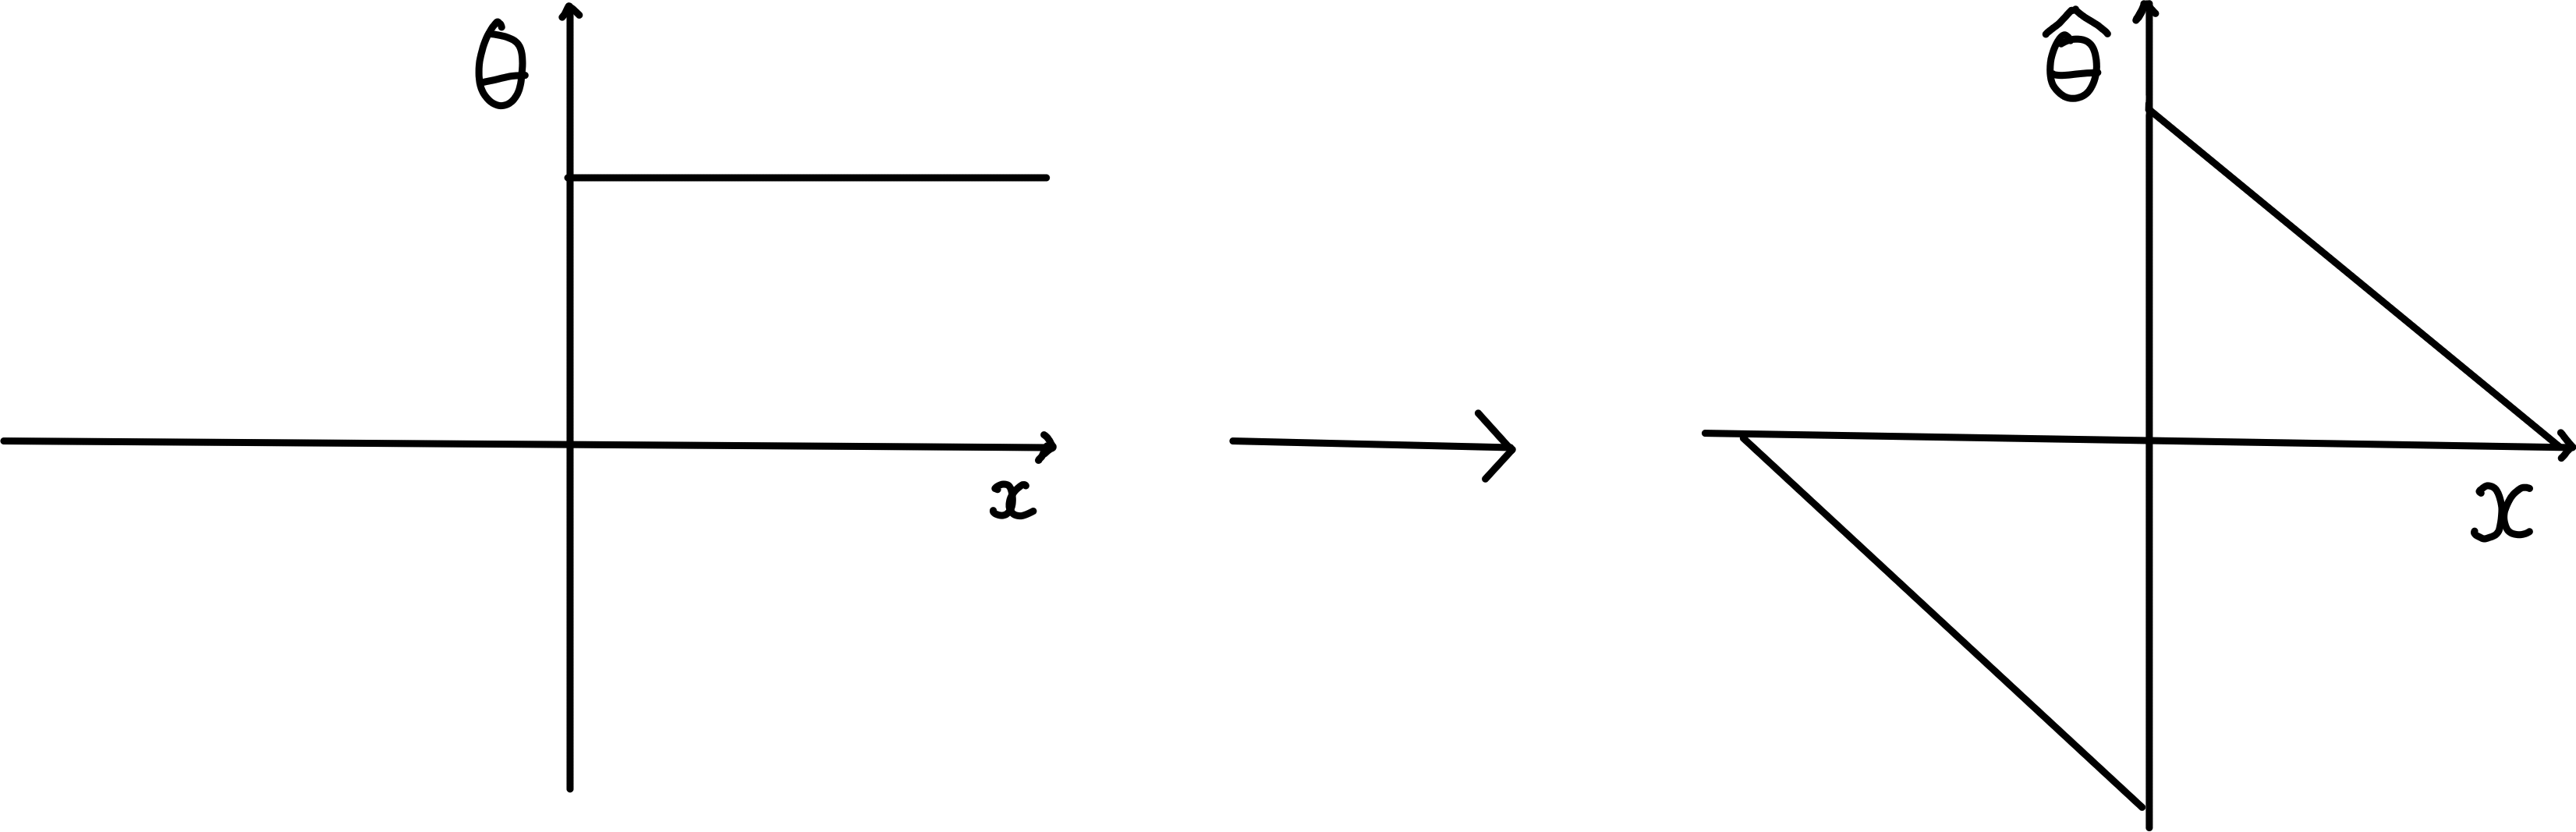
\includegraphics[height=5cm]{04-transformbcs} 
\end{figure}

\subsubsection{Seperation of variables}
We will now separate variables in the usual way.
We will consider the ansatz
\begin{align} \label{eq:4.12}
	\hat \theta(x,t) = X(x) T(t) \implies X'' = - \lambda X; \dot T = -D \lambda T
\end{align}
The boundary conditions imply $\lambda > 0$ and give the Fourier modes $X(x) = A \cos \sqrt{\lambda} x + B \sin \sqrt{\lambda} x$.
For $\cos \sqrt{\lambda} L = 0$, we require $\sqrt{\lambda_m} = \frac{m \pi}{2L}$ for $m$ odd.
Also, $\sin \sqrt{\lambda} L = 0$ gives $\sqrt{\lambda_n} = \frac{n \pi}{L}$ for $n$ even.
Since $\hat \theta$ is odd due to our initial conditions, we can take
\begin{align*}
	X_n = B_n \sin \frac{n \pi x}{L}; \quad \lambda_n = \frac{n^2 \pi^2}{L^2}
\end{align*}
Substituting $\lambda_n$ into \cref{eq:4.12}, $\dot T = -D \lambda T$, we have
\begin{align*}
	T_n(t) = C_n \exp(-\frac{Dn^2 \pi^2}{L^2} t ).
\end{align*}
In general, the solution is
\begin{align*}
	\hat \theta(x,t) = \sum_{n=1}^\infty b_n \sin \frac{n \pi x}{L} \exp(-\frac{Dn^2 \pi^2}{L^2} t )
\end{align*}

\subsection{Particular solution to diffusion equation}
Recall that
\begin{align*}
	\hat \theta(x,t) = \sum_{n=1}^\infty b_n \sin \frac{n \pi x}{L} \exp(-\frac{Dn^2 \pi^2}{L^2} t )
\end{align*}
At $t = 0$, we have a pure Fourier sine series.
We can then impose the initial conditions, to give
\begin{align*}
	b_n = \frac{1}{L} \int_{-L}^L \hat \phi(x,0) \sin \frac{n \pi x}{L} \dd{x}
\end{align*}
where
\begin{align*}
	\hat\phi(x,0) = H(x) - \frac{x+L}{2L}
\end{align*}
Hence, we can use the half-range sine series and find
\begin{align*}
	b_n = \underbrace{ \frac{2}{L} \int_0^L \qty(H(x) = \frac{1}{2}) \sin \frac{n \pi x}{L} \dd{x} }_{\text{square wave}/2} - \underbrace{ \frac{2}{L}\frac{x}{2L} \sin \frac{n \pi x}{L} \dd{x} }_{\text{sawtooth}/2L}
\end{align*}
which gives
\begin{align*}
	b_n = \frac{2}{(2m-1)\pi} - \frac{(-1)^{n+1}}{n\pi}
\end{align*}
where $n = 2m - 1$, and the first term vanishes for $n$ even.
For $n$ odd or even, we find the same result
\begin{align*}
	b_n = \frac{1}{n\pi}
\end{align*}
Hence
\begin{align*}
	\hat\theta(x,t) = \sum_{n=1}^\infty \frac{1}{n \pi} \sin \frac{n \pi x}{L} e^{-D \frac{n^2 \pi^2}{L^2} t}
\end{align*}
For the inhomogeneous boundary conditions,
\begin{align*}
	\theta(x,t) = \frac{x+L}{2L} + \sum_{n=1}^\infty \frac{1}{n \pi} \sin \frac{n \pi x}{L} e^{-D \frac{n^2 \pi^2}{L^2} t}
\end{align*}
The similarity solution $\frac{1}{2}\qty(1 + \erf(\frac{x}{2\sqrt{Dt}}))$ is a good fit for early $t$, but it does not necessarily satisfy the boundary conditions, so for large $t$ it is a bad approximation.

\subsection{Laplace's equation}
Laplace's equation is
\begin{align*}
	\laplacian \phi = 0
\end{align*}
This equation describes (among others) steady-state heat flow, potential theory $F = -\grad{\phi}$, and incompressible fluid flow $v = \grad{\phi}$.
The equation is solved typically on a domain $D$, where boundary conditions are specified often on the boundary surface.
The Dirichlet boundary conditions fix $\phi$ on the boundary surface $\partial D$.
The Neumann boundary conditions fix $\hat n \cdot \grad{\phi}$ on $\partial D$.

\subsection{Laplace's equation in three-dimensional Cartesian coordinates}
In $\mathbb R^3$ with Cartesian coordinates, Laplace's equation becomes
\begin{align*}
	\pdv[2]{\phi}{x} + \pdv[2]{\phi}{y} + \pdv[2]{\phi}{z} = 0
\end{align*}
We seek separable solutions in the usual way:
\begin{align*}
	\phi(x,y,z) = X(x)Y(y)Z(z)
\end{align*}
Substituting,
\begin{align*}
	X''YZ + XY''Z + XYZ'' = 0
\end{align*}
Dividing by $XYZ$ as usual,
\begin{align*}
	\frac{X''}{X} = \frac{-Y''}{Y} - \frac{Z''}{Z} & = -\lambda_\ell                         \\
	\frac{Y''}{Y} = \frac{-Z''}{Z} - \frac{X''}{X} & = -\lambda_m                            \\
	\frac{Z''}{Z} = \frac{-X''}{X} - \frac{Y''}{Y} & = -\lambda_n = \lambda_\ell + \lambda_m
\end{align*}
From the eigenmodes, our general solution will be of the form
\begin{align*}
	\phi(x,y,z) = \sum_{\ell,m,n} a_{\ell mn} X_\ell(x) Y_m(y) Z_n(z)
\end{align*}
Consider steady ($\pdv{\phi}{t} = 0$) heat flow in a semi-infinite rectangular bar, with boundary conditions $\phi = 0$ at $x = 0$, $x = a$, $y = 0$ and $y = b$; and $\phi = 1$ at $z = 0$ and $\phi \to 0$ as $z \to \infty$.
We will solve for each eigenmode successively.
First, consider $X'' = -\lambda_\ell X$ with $X(0) = X(a) = 0$.
This gives
\begin{align*}
	\lambda_\ell = \frac{l^2 \pi^2}{a^2};\quad X_\ell = \sin \frac{\ell \pi x}{a}
\end{align*}
where $\ell > 0, \ell \in \mathbb N$.
By symmetry,
\begin{align*}
	\lambda_m = \frac{m^2 \pi^2}{b^2};\quad Y_m = \sin \frac{m \pi y}{b}
\end{align*}
For the $z$ mode,
\begin{align*}
	Z'' = -\lambda_n Z = (\lambda_\ell + \lambda_m) Z = \pi^2\qty(\frac{\ell^2}{a^2} + \frac{m^2}{b^2}) Z
\end{align*}
Since $\phi \to 0$ as $z \to \infty$, the growing exponentials must vanish.
Therefore,
\begin{align*}
	Z_{\ell m} = \exp[-\qty(\frac{\ell^2}{a^2} + \frac{m^2}{b^2})^{1/2} \pi z]
\end{align*}
Thus the general solution is
\begin{align*}
	\phi(x,y,z) = \sum_{\ell, m} a_{\ell m} \sin \frac{\ell \pi x}{a} \sin \frac{m \pi y}{b} \exp[-\qty(\frac{\ell^2}{a^2} + \frac{m^2}{b^2})^{1/2} \pi z]
\end{align*}
Now, we will fix $a_{\ell m}$ using $\phi(x,y,0) = 1$ using the Fourier sine series.
\begin{align*}
	a_{\ell m} = \frac{2}{b} \int_0^b \frac{2}{a} \int_0^a \underbrace{1 \sin \frac{\ell \pi x}{a}}_{\text{square wave}} \underbrace{\sin \frac{m \pi y}{b}}_{\text{square wave}} \dd{x} \dd{y}
\end{align*}
So only the odd terms remain, giving
\begin{align*}
	a_{\ell m} = \frac{4a}{a(2k-1)\pi} \cdot \frac{4b}{b(2p-1) \pi}
\end{align*}
where $\ell = 2k-1$ is odd and $m = 2p-1$ is odd.
Simplifying,
\begin{align*}
	a_{\ell m} = \frac{16}{\pi^2 \ell m} \quad \text{ for } \ell, m \text{ odd}
\end{align*}
So the heat flow solution is
\begin{align*}
	\phi(x,y,z) = \sum_{\ell, m \text{ odd}} \frac{16}{\pi^2 \ell m} \sin \frac{\ell \pi x}{a} \sin \frac{\ell \pi y}{b} \exp[-\qty(\frac{\ell^2}{a^2} + \frac{m^2}{b^2})^{1/2} \pi z]
\end{align*}
As $z$ increases, every contribution but the lowest mode will be very small.
So low $\ell, m$ dominate the solution.

\subsection{Laplace's equation in plane polar coordinates}
In plane polar coordinates, Laplace's equation becomes
\begin{align*}
	\frac{1}{r} \pdv{r} \qty(r \pdv{\phi}{r}) + \frac{1}{r^2} \pdv[2]{\phi}{\theta} = 0
\end{align*}
Consider a separable form of the answer, given by
\begin{align*}
	\phi(r,\theta) = R(r) \Theta(\theta)
\end{align*}
We then have
\begin{align*}
	\Theta'' + \mu \Theta = 0;\quad r(rR')' - \mu R = 0
\end{align*}
The polar equation can be solved easily by considering periodic boundary conditions.
This gives $\mu = m^2$ and the eigenmodes
\begin{align*}
	\Theta_m(\theta) = \cos m \theta, \sin m \theta
\end{align*}
The radial equation is \textit{not} Bessel's equation, since there is no second separation constant.
We simply have
\begin{align*}
	r(rR')' - m^2 R = 0
\end{align*}
We will try a power law solution, $r = \alpha r^\beta$.
We find
\begin{align*}
	\beta^2 - m^2 = 0 \implies \beta = \pm m
\end{align*}
So the eigenfunctions are
\begin{align*}
	R_m(r) = r^m, r^{-m}
\end{align*}
which is one regular solution at the origin and one singular solution.
In the case $m = 0$, we have
\begin{align*}
	(rR') = 0 \implies rR' = \text{constant} \implies R = \log r
\end{align*}
So
\begin{align*}
	R_0(r) = \text{constant}, \log r
\end{align*}
The general solution is therefore
\begin{align*}
	\phi(r,\theta) = \frac{a_0}{2} + c_0 \log r + \sum_{m=1}^\infty \qty(a_m \cos m\theta + b_m \sin m\theta) r^m + \sum_{m=1}^\infty \qty(c_m \cos m\theta + d_m \sin m\theta) r^{-m}
\end{align*}
\begin{example}
	Consider a soap film on a unit disc.
	We wish to solve Laplace's equation with a vertically distorted circular wire of radius $r = 1$ with boundary conditions $\phi(1, \theta) = f(\theta)$.
	The $z$ displacement of the wire produces the $f(\theta)$ term.
	We wish to find $\phi(r,\theta)$ for $r < 1$, assuming regularity at $r = 0$.
	Then, $c_m = d_m = 0$ and the solution is of the form
	\begin{align*}
		\phi(r,\theta) = \frac{a_0}{2} + \sum_{m=1}^\infty \qty(a_m \cos m\theta + b_m \sin m\theta) r^m
	\end{align*}
	At $r = 1$,
	\begin{align*}
		\phi(1,\theta) = f(\theta) = \frac{a_0}{2} + \sum_{m=1}^\infty \qty(a_m \cos m\theta + b_m \sin m\theta)
	\end{align*}
	which is exactly the Fourier series.
	Thus,
	\begin{align*}
		a_m = \frac{1}{\pi} \int_0^{2\pi} f(\theta) \cos m \theta \dd{\theta};\quad b_m = \frac{1}{\pi} \int_0^{2\pi} f(\theta) \sin m \theta \dd{\theta}
	\end{align*}
	We can see from the equation that high harmonics are confined to have effects only near $r = 1$.
\end{example}

\subsection{Laplace's equation in cylindrical polar coordinates}
In cylindrical coordinates,
\begin{align*}
	\frac{1}{r} \pdv{r} \qty(r \pdv{\phi}{r}) + \frac{1}{4^2} \pdv[2]{\phi}{\theta} + \pdv[2]{\phi}{z} = 0
\end{align*}
With $\phi = R(r) \Theta(\theta) Z(z)$, we find
\begin{align*}
	\Theta'' = -\mu \Theta;\quad Z'' = \lambda Z;\quad r(rR')' + (\lambda r^2 - \mu) R = 0
\end{align*}
The polar equation can be easily solved by
\begin{align*}
	\mu_m = m^2;\quad \Theta_m(\theta) = \cos m\theta, \sin m\theta
\end{align*}
The radial equation is Bessel's equation, giving solutions
\begin{align*}
	R = J_m(kr), Y_m(kr)
\end{align*}
Setting boundary conditions in the usual way, defining $R=0$ at $r = a$ means that
\begin{align*}
	J_m(ka) = 0 \implies k = \frac{j_{mn}}{a}
\end{align*}
The radial solution is
\begin{align*}
	R_{mn}(r) = J_m\qty(\frac{j_{mn}}{a}r)
\end{align*}
We have eliminated the $Y_n$ term since we require $r = 0$ to give a finite $\phi$.
Finally, the $z$ equation gives
\begin{align*}
	Z'' = k^2 Z \implies Z = e^{-kz}, e^{kz}
\end{align*}
We typically eliminate the $e^{kz}$ mode due to boundary conditions, such as $Z \to 0$ as $z \to \infty$.
The general solution is therefore
\begin{align*}
	\phi(r,\theta,z) = \sum_{m=0}^\infty \sum_{n = 1}^\infty \qty(a_{mn} \cos m\theta + b_{mn} \sin m\theta) J_m\qty(\frac{j_{mn}}{a} r) e^{-frac{j_{mn}r}{a}}
\end{align*}

\subsection{Laplace's equation in spherical polar coordinates}
In spherical polar coordinates,
\begin{align*}
	\frac{1}{r^2} \pdv{r} \qty(r^2 \pdv{\Phi}{r}) + \frac{1}{r^2 \sin\theta}\pdv{\theta} \qty(\sin\theta \pdv{\Phi}{\theta}) + \frac{1}{r^2 \sin^2 \theta} \pdv[2]{\Phi}{\phi} = 0
\end{align*}
We will consider the \textit{axisymmetric case}; supposing that there is no $\phi$ dependence.
We seek a separable solution of the form
\begin{align*}
	\Phi(r,\theta) = R(r) \Theta(\theta)
\end{align*}
which gives
\begin{align*}
	(\sin\theta \Theta')' + \lambda \sin\theta \Theta = 0;\quad (r^2R')' - \lambda R = 0
\end{align*}
Consider the substitution $x = \cos\theta, \dv{x}{\theta} = -\sin\theta$ in the polar equation.
This gives $\dv{\Theta}{\theta} = -\sin\theta \dv{\Theta}{x}$ and hence
\begin{align*}
	-\sin\theta \dv{x}\qty[-\sin^2\theta \dv{\Theta}{x}] + \lambda \sin\theta \Theta = 0 \implies \dv{x}\qty[(1-x^2)\dv{\Theta}{x}] + \lambda \Theta = 0
\end{align*}
This gives Legendre's equation, so it has solutions of eigenvalues $\lambda_\ell = \ell (\ell + 1)$ and eigenfunctions
\begin{align*}
	\Theta_\ell(\theta) = P_\ell(x) = P_\ell(\cos\theta)
\end{align*}
The radial equation then gives
\begin{align*}
	(r^2 R')' - \ell (\ell + 1) R = 0
\end{align*}
We will seek power law solutions: $R = \alpha r^\beta$.
This gives
\begin{align*}
	\beta(\beta + 1) - \ell(\ell + 1) = 0 \implies \beta = \ell, \beta = -\ell - 1
\end{align*}
Thus the radial eigenmodes are
\begin{align*}
	R_\ell = r^{\ell}, r^{-\ell - 1}
\end{align*}
Therefore the general axisymmetric solution for spherical polar coordinates is
\begin{align*}
	\Phi(r,\theta) = \sum_{\ell = 0}^\infty (a_\ell r^{\ell} + b_\ell r^{-\ell - 1}) P_\ell(\cos\theta)
\end{align*}
The $a_\ell, b_\ell$ are determined by the boundary conditions.
Orthogonality conditions for the $P_\ell$ can be used to determine coefficients.
Consider a solution to Laplace's equation on the unit sphere with axisymmetric boundary conditions given by
\begin{align*}
	\Phi(1,\theta) = f(\theta)
\end{align*}
Given that we wish to find the interior solution, $b_n = 0$ by regularity.
Then,
\begin{align*}
	f(\theta) = \sum_{\ell=0}^\infty a_\ell P_\ell(\cos\theta)
\end{align*}
By defining $f(\theta) = F(\cos\theta)$,
\begin{align*}
	F(x) = \sum_{\ell=0}^\infty a_\ell P_\ell(x)
\end{align*}
We can then find the coefficients in the usual way, giving
\begin{align*}
	a_\ell = \frac{2\ell + 1}{2} \int_{-1}^1 F(x) P_{\ell}(x) \dd{x}
\end{align*}

\subsection{Generating function for Legendre polynomials}
Consider a charge at $r_0 = (x,y,z) = (0,0,1)$.
Then, the potential at a point $P$ becomes
\begin{align*}
	\Phi(r) & = \frac{1}{\abs{r - r_0}} = \frac{1}{(x^2 + y^2 + (x-1)^2)^{1/2}} \\
	& = \frac{1}{(r^2 (\sin^2 \phi + \cos^2 \phi) \sin^2 \theta + r^2 \cos^2 \theta - 2r \cos\theta + 1)^{1/2}} \\
	& = \frac{1}{(r^2 \sin^2 \theta + r^2 \cos^2 \theta - 2r \cos\theta + 1)^{1/2}} \\
	& = \frac{1}{(r^2 - 2r \cos\theta + 1)^{1/2}} \\
	& = \frac{1}{(r^2 - 2r \overline x + 1)^{1/2}}
\end{align*}
where 

$\overline x \equiv \cos \theta$.
This function $\Phi$ is a solution to Laplace's equation where $r \neq r_0$.
Note that we can represent any axisymmetric solution as a sum of Legendre polynomials.
Now,
\begin{align*}
	\frac{1}{\sqrt{r^2 - 2rx + 1}} = \sum_{\ell = 0}^\infty a_\ell P_\ell(x) r^\ell
\end{align*}
With the normalisation condition for the Legendre polynomials $P_\ell(1) = 1$, we find
\begin{align*}
	\frac{1}{1-r} = \sum_{\ell=0}^\infty a_\ell r^\ell
\end{align*}
Using the geometric series expansion, we arrive at $a_\ell = 1$.
This gives
\begin{align*}
	\frac{1}{\sqrt{r^2 - 2rx + 1}} = \sum_{\ell = 0}^\infty P_\ell(x) r^\ell
\end{align*}
which is the generating function for the Legendre polynomials.
    \section{The Laplace Equation}

\subsection{Laplace's equation}
Laplace's equation is
\begin{align} \label{eq:5.1}
	\laplacian \phi = 0
\end{align}
This equation describes (among others) steady-state heat flow, potential theory $F = -\grad{\phi}$, and incompressible fluid flow $v = \grad{\phi}$.
The equation \cref{eq:5.1} is solved typically on a domain $D$, where boundary conditions are specified often on the boundary surface.
The Dirichlet boundary conditions fix $\phi$ on the boundary surface $\partial D$.
The Neumann boundary conditions fix $\hat n \cdot \grad{\phi}$ on $\partial D$.

\subsection{Laplace's equation in three-dimensional Cartesian coordinates}
In $\mathbb R^3$ with Cartesian coordinates, Laplace's equation becomes
\begin{align} \label{eq:5.2}
	\pdv[2]{\phi}{x} + \pdv[2]{\phi}{y} + \pdv[2]{\phi}{z} = 0
\end{align}
We seek separable solutions in the usual way:
\begin{align*}
	\phi(x,y,z) = X(x)Y(y)Z(z)
\end{align*}
Substituting,
\begin{align*}
	X''YZ + XY''Z + XYZ'' = 0
\end{align*}
Dividing by $XYZ$ as usual,
\begin{align*}
	\frac{X''}{X} = \frac{-Y''}{Y} - \frac{Z''}{Z} & = -\lambda_\ell \quad \text{(constant)}\\
	\frac{Y''}{Y} = \frac{-Z''}{Z} - \frac{X''}{X} & = -\lambda_m \quad \text{(constant)} \\
	\frac{Z''}{Z} = \frac{-X''}{X} - \frac{Y''}{Y} & = -\lambda_n = \lambda_\ell + \lambda_m
\end{align*}
From the eigenmodes, our general solution will be of the form
\addtocounter{equation}{1}
\begin{align} \label{eq:5.4}
	\phi(x,y,z) = \sum_{\ell,m,n} a_{\ell mn} X_\ell(x) Y_m(y) Z_n(z)
\end{align}

\begin{example}[Steady heat conduction]
    Consider steady ($\pdv{\phi}{t} = 0$) heat flow\footnote{i.e. \cref{eq:4.3} with $\pdv{\phi}{t} = 0$ gives \cref{eq:5.1}} in a semi-infinite rectangular bar, with boundary conditions $\phi = 0$ at $x = 0$, $x = a$, $y = 0$ and $y = b$; and $\phi = 1$ at $z = 0$ and $\phi \to 0$ as $z \to \infty$.
    {\par
    \centering 
    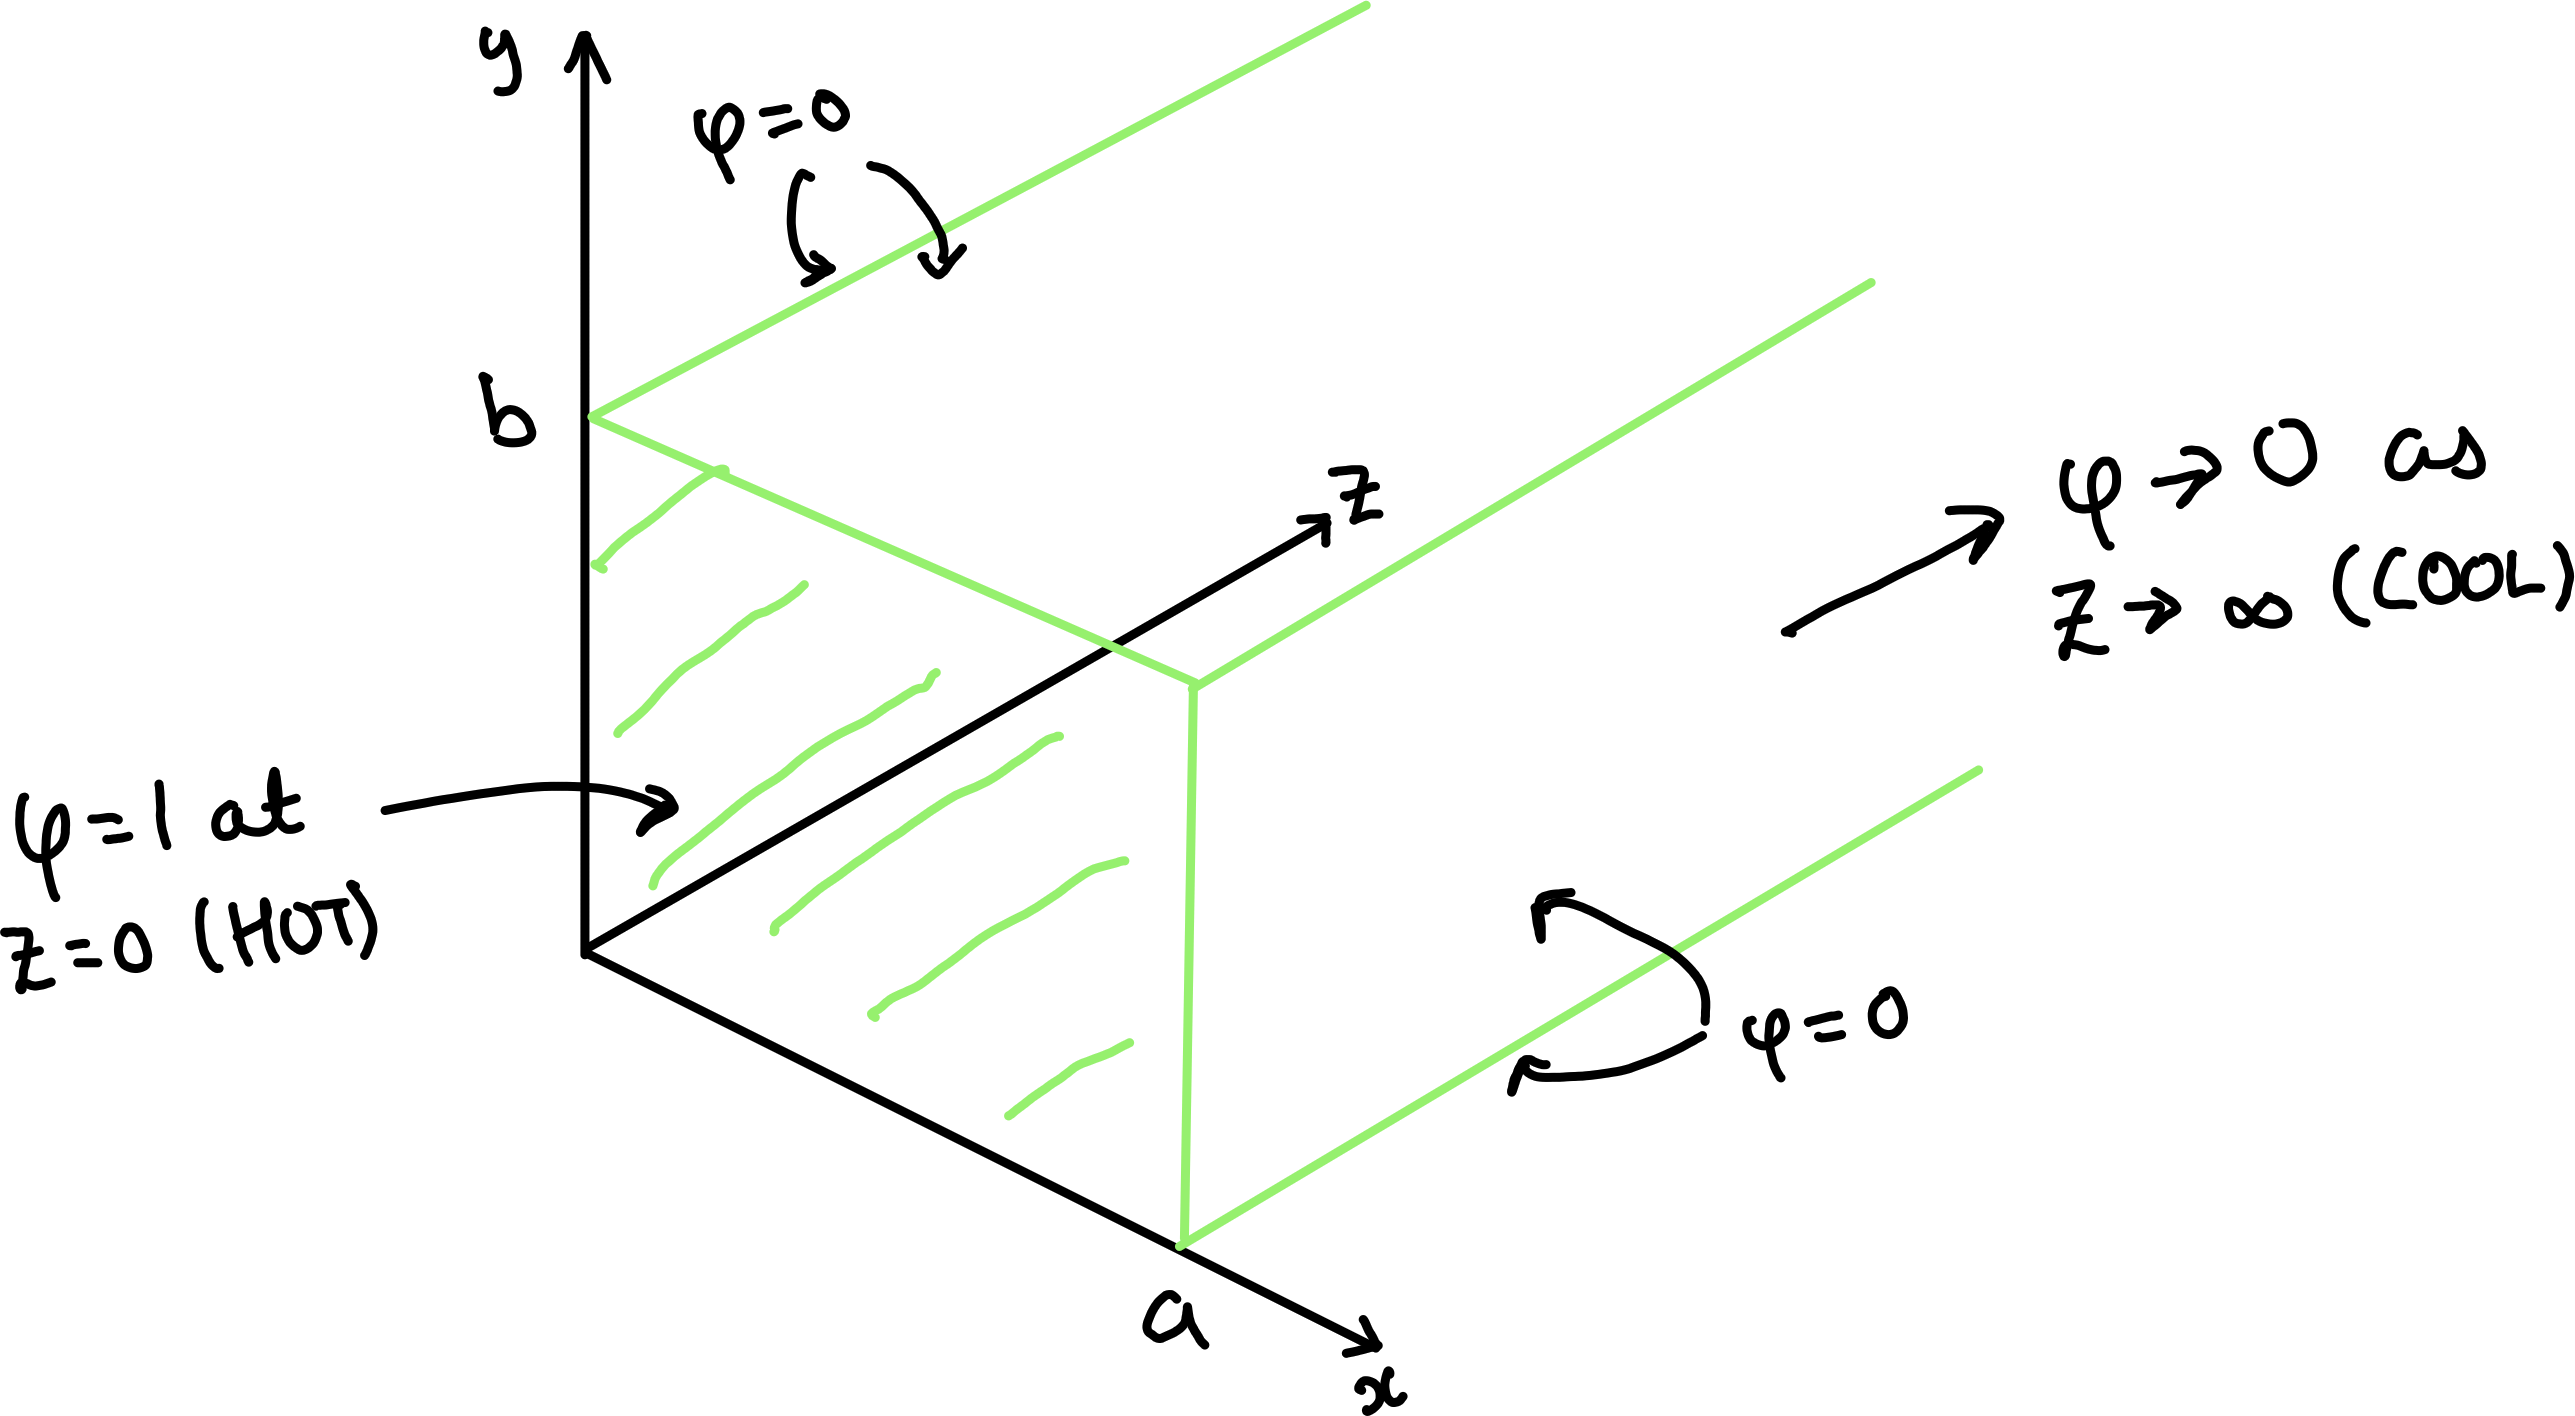
\includegraphics[height=5cm]{05-exm-steadyheat} 
    \par}
    We will solve for each eigenmode successively.
    First, consider $X'' = -\lambda_\ell X$ with $X(0) = X(a) = 0$.
    This gives
    \begin{align*}
        \lambda_\ell = \frac{l^2 \pi^2}{a^2};\quad X_\ell = \sin \frac{\ell \pi x}{a}
    \end{align*}
    where $\ell > 0, \ell \in \mathbb N$.
    By symmetry,
    \begin{align*}
        \lambda_m = \frac{m^2 \pi^2}{b^2};\quad Y_m = \sin \frac{m \pi y}{b}
    \end{align*}
    For the $z$ mode,
    \begin{align*}
        Z'' = -\lambda_n Z = (\lambda_\ell + \lambda_m) Z = \pi^2\qty(\frac{\ell^2}{a^2} + \frac{m^2}{b^2}) Z
    \end{align*}
    Since $\phi \to 0$ as $z \to \infty$, the growing exponentials must vanish.
    Therefore,
    \begin{align*}
        Z_{\ell m} = \exp[-\qty(\frac{\ell^2}{a^2} + \frac{m^2}{b^2})^{1/2} \pi z]
    \end{align*}
    Thus the general solution \cref{eq:5.4} becomes
    \begin{align*}
        \phi(x,y,z) = \sum_{\ell, m} a_{\ell m} \sin \frac{\ell \pi x}{a} \sin \frac{m \pi y}{b} \exp[-\qty(\frac{\ell^2}{a^2} + \frac{m^2}{b^2})^{1/2} \pi z]
    \end{align*}
    Now, we will fix $a_{\ell m}$ using $\phi(x,y,0) = 1$ using the Fourier sine series \cref{eq:1.12}.
    \begin{align*}
        a_{\ell m} = \frac{2}{b} \int_0^b \frac{2}{a} \int_0^a \underbrace{1 \sin \frac{\ell \pi x}{a}}_{\text{square wave}} \underbrace{\sin \frac{m \pi y}{b}}_{\text{square wave}} \dd{x} \dd{y}
    \end{align*}
    So only the odd terms remain, giving
    \begin{align*}
        a_{\ell m} = \frac{4a}{a(2k-1)\pi} \cdot \frac{4b}{b(2p-1) \pi}
    \end{align*}
    where $\ell = 2k-1$ is odd and $m = 2p-1$ is odd.
    Simplifying,
    \begin{align*}
        a_{\ell m} = \frac{16}{\pi^2 \ell m} \quad \text{ for } \ell, m \text{ odd}
    \end{align*}
    So the heat flow solution is
    \begin{align*}
        \phi(x,y,z) = \sum_{\ell, m \text{ odd}} \frac{16}{\pi^2 \ell m} \sin \frac{\ell \pi x}{a} \sin \frac{\ell \pi y}{b} \exp[-\qty(\frac{\ell^2}{a^2} + \frac{m^2}{b^2})^{1/2} \pi z]
    \end{align*}
    As $z$ increases, every contribution but the lowest mode will be very small.
    So low $\ell, m$ dominate the solution.

    Cross sectionals:
    insertpicture
\end{example} 

\subsection{Laplace's equation in plane polar coordinates}
In plane polar coordinates, Laplace's equation becomes
\addtocounter{equation}{1}
\begin{align} \label{eq:5.6}
	\frac{1}{r} \pdv{r} \qty(r \pdv{\phi}{r}) + \frac{1}{r^2} \pdv[2]{\phi}{\theta} = 0
\end{align}
Consider a separable form of the answer, given by
\begin{align*}
	\phi(r,\theta) = R(r) \Theta(\theta)
\end{align*}
We then have
\begin{align*}
	\Theta'' + \mu \Theta = 0;\quad r(rR')' - \mu R = 0
\end{align*}

\subsubsection{Polar equation}
The polar equation can be solved easily by considering periodic boundary conditions.
This gives $\mu = m^2$ and the eigenmodes as in \cref{eq:3.25}
\begin{align*}
	\Theta_m(\theta) = \cos m \theta, \sin m \theta
\end{align*}

\subsubsection{Radial equation}
The radial equation is \textit{not} Bessel's equation, since there is no second separation constant.
We simply have
\begin{align} \label{eq:5.7}
	r(rR')' - m^2 R = 0
\end{align}
We will try a power law solution, $R = \alpha r^\beta$.
We find
\begin{align*}
	\beta^2 - m^2 = 0 \implies \beta = \pm m
\end{align*}
So the eigenfunctions are
\begin{align*}
	R_m(r) = r^m, r^{-m}
\end{align*}
which is one regular solution at the origin and one singular solution. \\
In the case $m = 0$, we have
\begin{align*}
	(rR')' = 0 \implies rR' = \text{constant} \implies R = \log r
\end{align*}
So
\begin{align*}
	R_0(r) = \text{constant or } \log r
\end{align*}
The general solution is therefore
\begin{align} \label{eq:5.8}
	\phi(r,\theta) = \frac{a_0}{2} + c_0 \log r + \sum_{m=1}^\infty \qty(a_m \cos m\theta + b_m \sin m\theta) r^m + \sum_{m=1}^\infty \qty(c_m \cos m\theta + d_m \sin m\theta) r^{-m}
\end{align}

\begin{example}[Soap Film on a Unit Disc]
    insertpicture

	Consider a soap film on a unit disc.
	We wish to solve Laplace's equation \cref{eq:5.6} with a vertically distorted circular wire of radius $r = 1$ with boundary conditions $\phi(1, \theta) = f(\theta)$.
	The $z$ displacement of the wire produces the $f(\theta)$ term.
	We wish to find $\phi(r,\theta)$ for $r < 1$, assuming regularity at $r = 0$.
	Then, $c_m = d_m = 0$ and so \cref{eq:5.8} becomes
	\begin{align*}
		\phi(r,\theta) = \frac{a_0}{2} + \sum_{m=1}^\infty \qty(a_m \cos m\theta + b_m \sin m\theta) r^m
	\end{align*}
	At $r = 1$,
	\begin{align*}
		\phi(1,\theta) = f(\theta) = \frac{a_0}{2} + \sum_{m=1}^\infty \qty(a_m \cos m\theta + b_m \sin m\theta)
	\end{align*}
	which is exactly the Fourier series.
	Thus by \cref{eq:1.5},
	\begin{align*}
		a_m = \frac{1}{\pi} \int_0^{2\pi} f(\theta) \cos m \theta \dd{\theta};\quad b_m = \frac{1}{\pi} \int_0^{2\pi} f(\theta) \sin m \theta \dd{\theta}
	\end{align*}
	We can see from the equation that high harmonics are confined to have effects only near $r = 1$.
\end{example}

\begin{figure}[h] 
    \centering 
    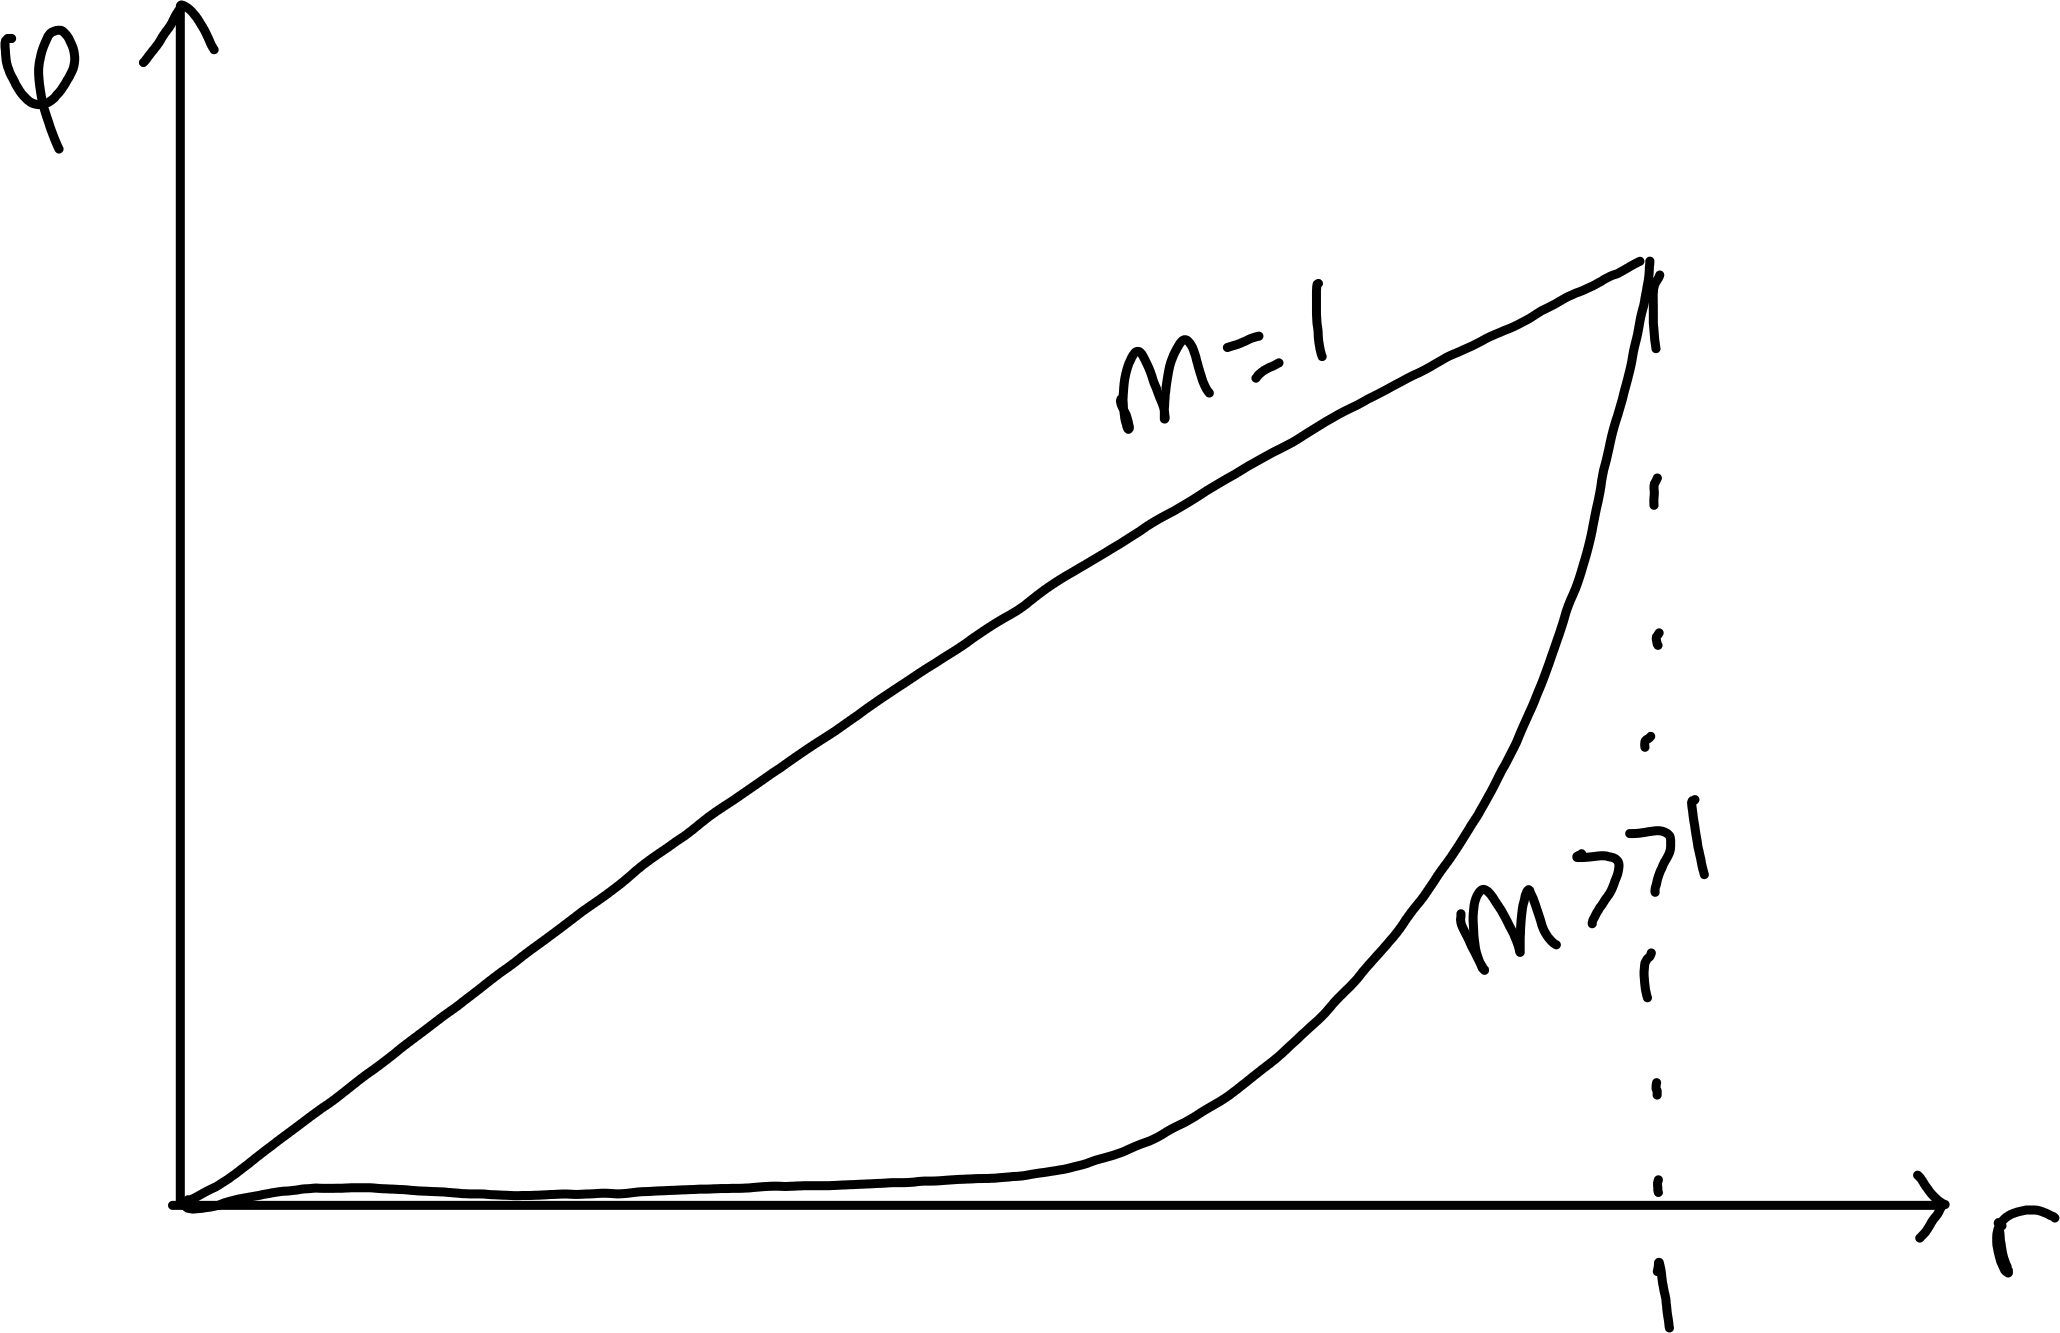
\includegraphics[height=5cm]{05-polarsoln} 
\end{figure}

\subsection{Laplace's equation in cylindrical polar coordinates}
In cylindrical coordinates,
\begin{align*}
	\frac{1}{r} \pdv{r} \qty(r \pdv{\phi}{r}) + \frac{1}{4^2} \pdv[2]{\phi}{\theta} + \pdv[2]{\phi}{z} = 0
\end{align*}
With $\phi = R(r) \Theta(\theta) Z(z)$, we find
\begin{align*}
	\Theta'' = -\mu \Theta;\quad Z'' = \lambda Z;\quad r(rR')' + (\lambda r^2 - \mu) R = 0
\end{align*}
The polar equation can be easily solved by
\begin{align*}
	\mu_m = m^2;\quad \Theta_m(\theta) = \cos m\theta, \sin m\theta
\end{align*}
The radial equation is Bessel's equation, giving solutions
\begin{align*}
	R = J_m(kr), Y_m(kr)
\end{align*}
Setting boundary conditions in the usual way, defining $R=0$ at $r = a$ means that
\begin{align*}
	J_m(ka) = 0 \implies k = \frac{j_{mn}}{a}
\end{align*}
The radial solution is
\begin{align*}
	R_{mn}(r) = J_m\qty(\frac{j_{mn}}{a}r)
\end{align*}
We have eliminated the $Y_n$ term since we require $r = 0$ to give a finite $\phi$.
Finally, the $z$ equation gives
\begin{align*}
	Z'' = k^2 Z \implies Z = e^{-kz}, e^{kz}
\end{align*}
We typically eliminate the $e^{kz}$ mode due to boundary conditions, such as $Z \to 0$ as $z \to \infty$.
The general solution is therefore
\begin{align*}
	\phi(r,\theta,z) = \sum_{m=0}^\infty \sum_{n = 1}^\infty \qty(a_{mn} \cos m\theta + b_{mn} \sin m\theta) J_m\qty(\frac{j_{mn}}{a} r) e^{-frac{j_{mn}r}{a}}
\end{align*}

\subsection{Laplace's equation in spherical polar coordinates}
In spherical polar coordinates,
\begin{align*}
	\frac{1}{r^2} \pdv{r} \qty(r^2 \pdv{\Phi}{r}) + \frac{1}{r^2 \sin\theta}\pdv{\theta} \qty(\sin\theta \pdv{\Phi}{\theta}) + \frac{1}{r^2 \sin^2 \theta} \pdv[2]{\Phi}{\phi} = 0
\end{align*}
We will consider the \textit{axisymmetric case}; supposing that there is no $\phi$ dependence.
We seek a separable solution of the form
\begin{align*}
	\Phi(r,\theta) = R(r) \Theta(\theta)
\end{align*}
which gives
\begin{align*}
	(\sin\theta \Theta')' + \lambda \sin\theta \Theta = 0;\quad (r^2R')' - \lambda R = 0
\end{align*}
Consider the substitution $x = \cos\theta, \dv{x}{\theta} = -\sin\theta$ in the polar equation.
This gives $\dv{\Theta}{\theta} = -\sin\theta \dv{\Theta}{x}$ and hence
\begin{align*}
	-\sin\theta \dv{x}\qty[-\sin^2\theta \dv{\Theta}{x}] + \lambda \sin\theta \Theta = 0 \implies \dv{x}\qty[(1-x^2)\dv{\Theta}{x}] + \lambda \Theta = 0
\end{align*}
This gives Legendre's equation, so it has solutions of eigenvalues $\lambda_\ell = \ell (\ell + 1)$ and eigenfunctions
\begin{align*}
	\Theta_\ell(\theta) = P_\ell(x) = P_\ell(\cos\theta)
\end{align*}
The radial equation then gives
\begin{align*}
	(r^2 R')' - \ell (\ell + 1) R = 0
\end{align*}
We will seek power law solutions: $R = \alpha r^\beta$.
This gives
\begin{align*}
	\beta(\beta + 1) - \ell(\ell + 1) = 0 \implies \beta = \ell, \beta = -\ell - 1
\end{align*}
Thus the radial eigenmodes are
\begin{align*}
	R_\ell = r^{\ell}, r^{-\ell - 1}
\end{align*}
Therefore the general axisymmetric solution for spherical polar coordinates is
\begin{align*}
	\Phi(r,\theta) = \sum_{\ell = 0}^\infty (a_\ell r^{\ell} + b_\ell r^{-\ell - 1}) P_\ell(\cos\theta)
\end{align*}
The $a_\ell, b_\ell$ are determined by the boundary conditions.
Orthogonality conditions for the $P_\ell$ can be used to determine coefficients.
Consider a solution to Laplace's equation on the unit sphere with axisymmetric boundary conditions given by
\begin{align*}
	\Phi(1,\theta) = f(\theta)
\end{align*}
Given that we wish to find the interior solution, $b_n = 0$ by regularity.
Then,
\begin{align*}
	f(\theta) = \sum_{\ell=0}^\infty a_\ell P_\ell(\cos\theta)
\end{align*}
By defining $f(\theta) = F(\cos\theta)$,
\begin{align*}
	F(x) = \sum_{\ell=0}^\infty a_\ell P_\ell(x)
\end{align*}
We can then find the coefficients in the usual way, giving
\begin{align*}
	a_\ell = \frac{2\ell + 1}{2} \int_{-1}^1 F(x) P_{\ell}(x) \dd{x}
\end{align*}

\subsection{Generating function for Legendre polynomials}
Consider a charge at $r_0 = (x,y,z) = (0,0,1)$.
Then, the potential at a point $P$ becomes
\begin{align*}
	\Phi(r) & = \frac{1}{\abs{r - r_0}} = \frac{1}{(x^2 + y^2 + (x-1)^2)^{1/2}} \\
	& = \frac{1}{(r^2 (\sin^2 \phi + \cos^2 \phi) \sin^2 \theta + r^2 \cos^2 \theta - 2r \cos\theta + 1)^{1/2}} \\
	& = \frac{1}{(r^2 \sin^2 \theta + r^2 \cos^2 \theta - 2r \cos\theta + 1)^{1/2}} \\
	& = \frac{1}{(r^2 - 2r \cos\theta + 1)^{1/2}} \\
	& = \frac{1}{(r^2 - 2r \overline x + 1)^{1/2}}
\end{align*}
where 

$\overline x \equiv \cos \theta$.
This function $\Phi$ is a solution to Laplace's equation where $r \neq r_0$.
Note that we can represent any axisymmetric solution as a sum of Legendre polynomials.
Now,
\begin{align*}
	\frac{1}{\sqrt{r^2 - 2rx + 1}} = \sum_{\ell = 0}^\infty a_\ell P_\ell(x) r^\ell
\end{align*}
With the normalisation condition for the Legendre polynomials $P_\ell(1) = 1$, we find
\begin{align*}
	\frac{1}{1-r} = \sum_{\ell=0}^\infty a_\ell r^\ell
\end{align*}
Using the geometric series expansion, we arrive at $a_\ell = 1$.
This gives
\begin{align*}
	\frac{1}{\sqrt{r^2 - 2rx + 1}} = \sum_{\ell = 0}^\infty P_\ell(x) r^\ell
\end{align*}
which is the generating function for the Legendre polynomials.

    \part{Inhomogenous ODEs and Greens Functions}
\end{document}